%\documentclass{report}
\documentclass[12pt,a4paper]{report}
\usepackage[utf8]{inputenc}
\usepackage{subfiles}
\usepackage{graphicx}
\usepackage[margin = 1in]{geometry}
\usepackage{fixltx2e}
\usepackage{amsmath}
\usepackage{amsfonts}
\usepackage{amssymb}
\usepackage{cite}
\usepackage{textcomp}
\usepackage{url}
\usepackage{caption}
\usepackage{parskip}
\usepackage{listings}
\usepackage{tabularx}
\usepackage{enumitem}


\parindent=0pt

\usepackage[toc,page]{appendix}
\usepackage{hyperref}

%\title{\bf CS409 - Group Report}
\title{Indoor Localisation and Navigation Using Inertial Sensors on Smartphones}
\author{Pedram Amirkhalili, Joey Benrimoj,  Dominic Brown, Varun Golani, \\Robert Hubinsky and Daniel Seabright  } 
\date{}
\setcounter{tocdepth}{3}


\begin{document}
\maketitle
%\line(1,0){450}

\tableofcontents

\pagebreak

\begin{abstract}
This report documents the work carried out in the creation of an internal navigation mobile application that makes exclusive use of a smartphone's intertial sensors, built for navigation through the University of Warwick's Computer Science Department building. This involves the use of a custom built step detector to register movement and the compass to measure a user's heading. This is followed by an analysis of its overall performance and a critique of the software development resources provided for both iPhone and Android application development, primarily through the Xamarin development kit.
\end{abstract}

\chapter{Introduction}

Navigation is the process of accurately determining a person's location and then planning out movements through possible paths to a desired destination~\cite{navMeaning}. Historically, this has been a problem that has been tackled mainly for the case of exterior navigation. From the more primitive use of stars on sea voyages hundreds of years ago, to the use of technology today, exterior navigation has been solved in large part through the use of satellite navigation systems. The best known and most popular of these is the Global Positioning System (GPS), navigation technology that is used in almost every sea vessel, plane and motor vehicle that exists today~\cite{gps}.\\

The development of smartphones has resulted in many of them now also being fitted with a GPS unit, allowing navigation to be available to anyone at any time. Issues exist however with GPS signals penetrating through buildings~\cite{gps}, limiting their usefulness for navigation within indoor environments. Indeed, even if signals were able to make their way indoors, the margins of error associated with GPS technology (running into the tens of metres) means that this would likely prove to be ineffective for navigation anyway, considering the smaller overall distances involved, between doors for example, when compared to exterior navigation, where distances between buildings are larger.\\

Despite this, a similarly comprehensive alternative to GPS for interior navigation has yet to be devised.

\section{Motivation}

The primary motivation for this project lay in the fact that indoor navigation is a problem that still remains relatively unsolved. Despite a wide range of proposed solutions making use of different technologies, no solution can claim the same kind of universal acceptance that GPS has within the world of exterior navigation. This is especially true for a solution that makes exclusive use of smartphones. As far as we are aware, there is no low cost, user friendly application for smartphones that is able to accurately navigate a user through indoor environments. As such, we were attracted by the prospect of being able to contribute in our own way to the advancement of technology by tackling such an open problem.

A solution would also have a myriad of real world applications. Users within large, unfamiliar public buildings could be directed to specific rooms with indoor navigation. Tourists that are visiting historical sites or museums may use such an application to be directed along tour paths tailored to their specific interests. Users in shopping centres could also be directed to desired stores, with user routing data possibly being used to inform research on consumer behaviour and influence the design of better shopping centres or marketing campaigns. So not only is the problem of effective indoor navigation through the use of smartphones an open one, the pursuit of a solution can also be deemed a worthwhile endeavour.

\section{Objectives}

For this project we proposed the development of a smartphone application that is able to track and navigate a user within an indoor environment. For the purposes of the project, the indoor environment was defined as the University of Warwick's Computer Science Department building. The following objectives were set:\\

\begin{itemize}
\item Inertial Sensors - The application should make exclusive use of a smartphone's inertial sensors in order to track a user's movement. This means not considering solutions that involve use of WiFi signals, bluetooth beacons, or any other kind of input that would depend on external hardware. We wished the eventual solution to be self sufficient, and only require the user and their smartphone (which would include building floor plans that are pre loaded into the smartphone).

\item Accuracy - The navigation should be accomplished to a reasonable degree of accuracy. Anything more than a few metres could result in users being directed to the wrong location. The application should be able to guide users to a correct destination at a consistent level.

\item User Interface - An effective solution should have an intuitive and attractive user interface. The application should display the user's location and the path that must be followed in an appealing and easy to read manner. The floor plans used need to be carefully designed and the interface should feel professionally crafted and not like a proof of concept placeholder.

\end{itemize}

\chapter{Existing Solutions}

Many solutions have been proposed for the problem of indoor navigation. Within this section we shall be documenting some of the most popular of these.

\section{Dead Reckoning Using a Step Detection Algorithm}

\section{Landmark System}

\section{Landmarks}

Landmarks have long been tools used for navigation, prior to the creation of smartphones and other technologies. It should then be of no surprise that some navigation methods for smartphones have adopted these as the core of how they operate. For the purposes of this project, two different classes of landmark based systems were examined:

\begin{enumerate}
	\item \textbf{Beacon/Non-Organic Landmarks} - This is where wireless beacons are placed in the environment and the device uses them to determine its location
	\item \textbf{Organic Landmarks} - This a system that uses landmarks that have been identified to be within the environment, such as WiFi routers and elevators.
\end{enumerate}

Note the term Organic is a reference to the landmark being present in the environment without the need for the development team to place an object or device to create the waypoint.

An example of a Beacon based system is one developed by Inoue. Y, et. al ~\cite{Inoue2009} which works autonomously, removing the need for additional infrastructure in the form of a server. The beacons in this project are self-sufficient devices with their own power sources and transmitters, meaning that the required infrastructure is low-cost and can be placed in any location.

Prior to using the devices, three sets of reference data are required:

\begin{enumerate}
	\item \textbf{Pedestrian Network Data} - Data that defines where a pedestrian can walk within the specified environment.
	\item \textbf{Building Map Data} - The floor plan for the building.
	\item \textbf{Received Signal Strength (RSS) Fingerprint Data} - Data that helps with locational calculations.
\end{enumerate}

The RSS Fingerprint Data is obtained by measuring the RSS at fixed points in the environment for every beacon. From the reference data and real-time beacon signal data it is then possible to calculate where the user should be located. This application uses a series of particle filters to then estimate a position and keep updating it as new beacon data is received.

Whilst this approach reduces the amount of infrastructure normally required for beacon based approaches by not requiring a server, it still requires the placement of devices in the environment. This combined with the focus not being on the use of inertial sensors for navigation make it unviable for the scope of our requirements.

With Organic Landmarks the issue of not fitting the requirements of using inertial sensors is removed, since there are no longer devices placed in the environment to help with locational calculations. There are two ways in which organic landmarks can be used for navigation, the first is to use landmarks that can be detected using sensors and then reset the error in the system and the user's location. The second is to use computer vision to identify landmarks and through this keep track of the user. This second method goes beyond the scope of our project and was therefore not researched beyond simple acknowledgement.

An example of a system that uses ``discovered'' landmarks is UnLoc, proposed by Wang. H, et al. ~\cite{wang2012no}, which works by using a combination of Dead Reckoning to detect where the user is moving and Landmarks to reset the error that builds up with such a system. Landmarks are either identified through examining floor plans or by searching through the environment for unique sensor readings that correspond to a specific region. Some of the utilised landmarks are the following:

\begin{itemize}
	\item Elevators
	\item Stairs
	\item WiFi Routers
	\item Areas of Specific Magnetic Signals
\end{itemize}

This system is shown to work well in negating the error present in Dead Reckoning and maintaining an accurate user location. Since the landmarks used are present within the University of Warwick Computer Science building, we felt this warranted further investigation during development.

\section{Beacon Based Location Triangulation}

\section{Magnetic Navigation Mapping}
 
Less traditional solutions to the indoor navigation problem have also recently been proposed. One of the most promising and strongly tipped to be leading towards an eventual scalable and comprehensive solution at the level of GPS is an Indoor Positioning System (IPS) developed by a company called IndoorAtlas~\cite{indoorAtlas}. The company is comprised of researchers and PhD students from the University of Oulu in Finland, and draws from over ten years of research conducted by the university into the movements of animals via their interaction with the Earth's magnetic field, and how this can be translated into technology~\cite{IAReport}.
 
Animals like homing pigeons have been known to make use of the Earth's magnetic field to aid them in their navigation. They contain tiny particles of iron oxide called magnetite within their beaks that allows them to sense magnetic fields and ascertain where magnetic north lies~\cite{pigeon}. This gives them an uncanny sense of direction, with similar abilities also having been observed within lobsters. 
 
IndoorAtlas makes use of a similar concept. The Earth's magnetic field exists everywhere and is modulated by man-made structures and objects. The application provided by the company maps out the magnetic field variations across buildings, with the magnetometer within smartphones then being used to record the magnetic information of the user's position and their position matched to the mapped out readings~\cite{IAReport}.
 
For this to be possible, floor plans of the target buildings are first produced. Then users carrying smartphones operating the software map out the area with the magnetometer. Theoretically, any user who then visits the area is able to download the pre built magnetic map and then be tracked. A smartphone's magnetometer is able to produce a magnetic map to an accuracy of up to 0.1cm, with final system navigation accuracy claimed to be between 0.1 and 2 metres. 
 
One of the most exciting prospects of such a solution is the lack of a need for external infrastructure. Whereas other solutions produced by Google and Nokia make use of WiFi hotspots or bluetooth beacons, which by definition require external infrastructure, the IndoorAtlas solution only requires a smartphone. Magnetic fields are also present everywhere, whereas WiFi and bluetooth would be infeasible in places like underground metro systems (ironically it would be places like these that might benefit the most by having an effective IPS system directing people efficiently).
 
Several problems exist with this method though. Principle amongst these is the fact that magnetic fields change over time. These fields are dictated largely by iron that sits molten deep within the earth. As this molten iron shifts, so too do the magnetic fields. Local changes in magnetic field are also caused by the addition of buildings within the vicinity of the target building and even changes to its own interior arrangement. This results in collected data becoming obsolete before too long.
 
 A provided workaround to this problem is to create a network of users that continuously update the magnetic map information. Borrowing the concept of Simultaneous Location and Mapping (SLAM), this would involve either providing users with instructions about how to update local magnetic maps within already established locations, or implementing an advanced automatic update system that uses previous known locations and incorrectly matching readings to update the magnetic maps in an automated manner. The latter, though more complex, would theoretically mean that any shifts in magnetic field within popular locations that are traversed regularly by users would always be picked up and updated and provide accurate navigational information~\cite{IAReport}.
 
 Access to floor plans might also be problematic. Privacy concerns coupled with the vast amount of buildings that could be eligible for such a solution means that this is a further barrier to this technology really taking hold.
 
Although exciting, we felt as a group that a similarly styled solution would not be the most appropriate for our project. The technology is very much in its infancy and grounded as of now in the theoretical. 10 years of research has resulted in the beginnings of a system that might one day see a commercial use, with many years of hard work still required to get the technology anywhere near the level that GPS was even 15 or 20 years ago. We felt that pursuing a solution that made use of magnetic maps was too ambitious for both our level of expertise and size of group and desired to come up with an application design that lay within more well trodden ground.

\chapter{Background Research}

 \section{Tracking user movement}

An obvious way to track user position is to perform double integration on the obtained acceleration to get distance travelled. However this results in introduction of error, as the result is only an approximation of the underlying signal. Furthermore, integration of the noise component leads to the standard deviation of the error in position increasing with integration time~\cite[p.73]{integrationError}. Thong, Y. K., et al.~\cite{integrationErrorPractical} analysed the practical effect that double integration of accelerometer noise has on this error by carrying out experiments using two commercial accelerometers, and found that this error very quickly accumulates with time~\cite[p.1168]{integrationErrorPractical}. As such, this approach is deemed unsuitable for a navigation system which continuously and precisely requires the user’s current position. Foxlin, E.'s approach~\cite{foxlin2005pedestrian} alleviates the integration error by using the concept of `zero-velocity updates (ZUPTs)’, which exploits the fact that there is a momentary stationary period of zero velocity and acceleration during walking motion when the user’s foot makes contact with the ground. This allows correction of the velocity error after each stride and makes the error accumulation ``linear in the number of steps''~\cite[p.38]{foxlin2005pedestrian}. This, however, requires a dedicated sensor to be placed on the user’s foot and does not come under the purview of a smartphone based approach. 

Most dead-reckoning systems thus make use of step detection to identify user movement and step length estimation to estimate their displacement and avoid the double integration problem. Existing approaches that make use of a smartphone’s inertial sensors typically restrict the phone’s position to two scenarios - the user having the phone in their pocket and/or in front of them in their hand. Steps are detected by identifying the consistent change in sensor readings, particularly the accelerometer, caused by rhythmic motion during walking. For instance, Wang, H., et al.~\cite{wang2012no} observe that the graph of magnitude readings of a 3-axis accelerometer follow a sinusoidal pattern corresponding to the ``natural up/down bounce of the human body for each step taken''~\cite[p.203]{wang2012no} in both the in-hand and pocket case. They then isolate individual steps through simple peak detection and thresholding in the graph. Li, F., et al.~\cite{li2012reliable} also use accelerometer magnitude in a similar manner to identify steps, subsequently applying heuristic constraints and dynamic time warping validation to reduce false positives.  

While taking the magnitude of the accelerometer allows the step detection procedure to be independent of the phone’s orientation, as a side effect, moving the phone along the axes that do not correspond to the user’s vertical movement can also produce similar sinusoidal patterns. Jin, Y., et al.~\cite{jin2011robust} isolate acceleration specifically along the required vertical axis by projecting the acceleration measurements from the phone’s local x-y-z axes to the East-North-Up (E-N-U) world co-ordinate system, where `Up' is the desired axis.  This is achieved by using the `rotation matrix' containing orientation measurements that are applied to the acceleration vector in the local co-ordinates. Once the accelerometer readings are obtained on this vertical axis they detect steps by identifying sequences of local maxima followed by local minima along with thresholding on both the time elapsed and absolute value difference between the two. 

Efforts have also been made to extend step detection to work in arbitrary phone positions, so that it can be used in real-world situations where the position varies as the user performs a multitude of activities. Such approaches either involve broadly identifying the type of activity the user is performing and then using the appropriate sensors for step detection in that particular situation, or generating and using one or more measures that already take into account the variations in position. Susi, M., et al.~\cite{susi2013motion} specify a set of possible user activities and associate with each one unique features based on measures derived from accelerometer and gyroscope readings. The user’s current activity is then identified by extracting the feature set corresponding to their motion and using a pre-defined decision tree to classify it as one of the specified activities. A specific version of the algorithm optimised for peak detection in the context of that particular activity is then used to detect steps. For instance, if the activity is classified as `phone in swinging hand' then gyroscope readings are also considered due to periodic rotation of the user’s arm. Conversely, activities such as texting do not involve any rotation and thus only accelerometer readings are looked at. Zeng, Q., et al.~\cite{zeng2015novel} proposed a novel step counting algorithm that works irrespective of the phone’s position and step mode (variation in the user’s motion, including walking and running). In addition to the accelerometer they also make use of the 3-axis gravity sensor, which provides acceleration acting on each of the axes specifically due to gravity. A change in these values signifies a change in the position/orientation of the phone and can be used to compensate for the resulting variance in accelerometer readings. Thus the authors take a linear combination of the accelerometer and gravity readings to produce a single metric incorporating this compensation, on the basis of which step detection is carried out. Lee, H., et al.~\cite{lee2015step} consider both the short and long term changes in accelerometer magnitude to capture the variations caused due to different positions and step modes. Peak/valley candidates are identified on the basis of measures that track these short/long term changes such as mean and standard deviation. Candidates are then validated using adaptive thresholds which ensure that sufficient time, corresponding to the estimated minimum duration between subsequent steps in standard motion, has elapsed between adjacent peaks and valleys. 

\section{Sensors}

\subsection{Accelerometer}
Existing approaches predominantly make use of the phone's accelerometer readings in order to detect the user's steps. As the name suggests, an accelerometer is a device that measures the acceleration that is applied to the device. In smartphones, this acceleration $A_{d}$ is measured using the relation in 
Equation~\ref{eq:accelerometerAcceleration}~\cite{accelerometerAcceleration}.  

\begin{equation}\label{eq:accelerometerAcceleration}
A_{d} = - \sum F_{s}/massAccelerometer
\end{equation}
\\
where $\sum F_{s}$ is the sum of the forces acting upon the device. Included in $F_{s}$ is the force acting on the device due to the Earth's gravity, which produces acceleration having a constant magnitude of $9.81 m/s^2$. 

In particular, most modern smartphones come equipped with a `3-axis' accelerometer, which reports the accelerations acting separately on the 3 principal axes of the phone's co-ordinate system - X, Y and Z. In Android and iOS these 3 axes are defined relative to the phone's screen when held in its `natural orientation', which is portrait in most cases. The axes are illustrated in Figure~\ref{fig:axisDevice}

\begin{center}
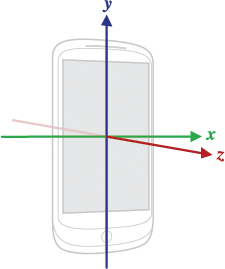
\includegraphics[scale=0.5]{images/axisDevice.png}
\captionof{figure}{The 3 principal axes of smartphones, defined with respect to the screen in its `natural orientation'~\cite{axisDevice}}
\label{fig:axisDevice}
\end{center}

As seen from the figure, the X-axis passes through the side of the phone, the Y-axis is along the vertical segment while the Z-axis projects out from the centre of the screen. The positions of these axes remain fixed with respect to the screen, and thus rotate accordingly along with change in the phone's orientation. 

\subsection{Gyroscope}
In addition to the accelerometer some approaches also consider the readings from the gyroscope, which is a sensor that measures the rate of rotation around the phone's principal axes~\cite{accelerometerAcceleration}. Such rotations can be correlated with the user's steps in certain situations, such as when the phone swings while the user has their hand to the side of their body while walking. Since we envisaged any final application to have the phone's position be in the user's hand and in front of them at all times, there would be no considerable rotational motion involved. Thus the gyroscope readings will not provide any meaningful information for step detection and they are not considered in our approach. 

\subsection{Barometer}

As smartphones continue to get more and more powerful, new sensors are added to the array they already have. In recent years the barometer is becoming more prevalent. This a sensor that can determine the air pressure surrounding the phone. With this information, it is possible to obtain a height above sea level for the phone based off the barometric formula, which models the relationship from pressure to altitude.

The application of this information has the potential to be very useful and influential for indoor navigation systems, as if accurate enough, a barometer would allow for more precise vertical positioning, allowing systems to keep track of users throughout several floors in large buildings. With this in mind, a team from Singapore Management University ~\cite{baro2014} set out to test if barometric sensors in phones could be used for this purpose.

In their study they tested numerous factors that could have an effect on the readings, finding that  time, weather and location had an effect on the pressure values the sensors recorded. Although this was expected, the team was surprised by the fact that even identical devices left next to one another would produce different pressure readings but with the same overall pattern. ~\cite[p.2]{baro2014}
%These three factors are expected to have an effect as it is well documented that weather has an effect on the pressure, and obviously with time and location the weather and conditions are likely to be given. The other unexpected factor that was found 

This led them to focus on the relative barometer reading (the differences between changes in readings) instead of the absolute one. This pressure difference is independent of all the above factors and therefore could be used to predict floor changes. After proving this was indeed the case, they moved on to recording a number of samples and used data analysis techniques to see if they could predict whether a floor had changed using just the difference in pressure values. With this they managed to achieve a 99.54\% accuracy.

This particular study proves the potential that the barometer has in terms of indoor navigation and keeping track of a user's verticality. However it is noted that floors need to have a minimum difference of 0.2hPa or 1.6 metres, as the maximum error in pressure differences was around this value. In a building, if the difference between floors is close to this value the probability of error increases.

Whilst this study proves that the barometer is useful, it is not the only system that showcases its uses. Another example of this is the iBaro-altimeter system developed at The University of Tokyo ~\cite{baro22014}. To calculate one's altitude another pressure reference point is needed as part of the barometric formula, often either obtained from a nearby local source (meteorological station) or through using a constant.

This system they proposed worked by using a series of standard reference points and other temporary ones they could ascertain to be correct, such as a smartphone in the system that they assigned an altitude to. These collected reference points are stored on a server. A smartphone which then wants its altitude makes a request with some required information.

Whilst this system achieved low error rates, it requires a large amount of infrastructure which does not fit with the idea behind our application. Even if the server could be removed from the design, an internet connection would be necessary to collect some of the reference points, and GPS location is one of the inputs that the server requires to return an altitude.

\subsection{Practical Research}

(ADD INTRO)

In order to confirm that the actual sensor readings correspond to the described behaviour we recorded and analysed accelerometer data from our own phones. The first recording was performed with the phone remaining stationary throughout and kept flat on the surface with the screen facing upwards. The readings obtained are shown in Figure~\ref{fig:accelerationZ}.

\begin{center}
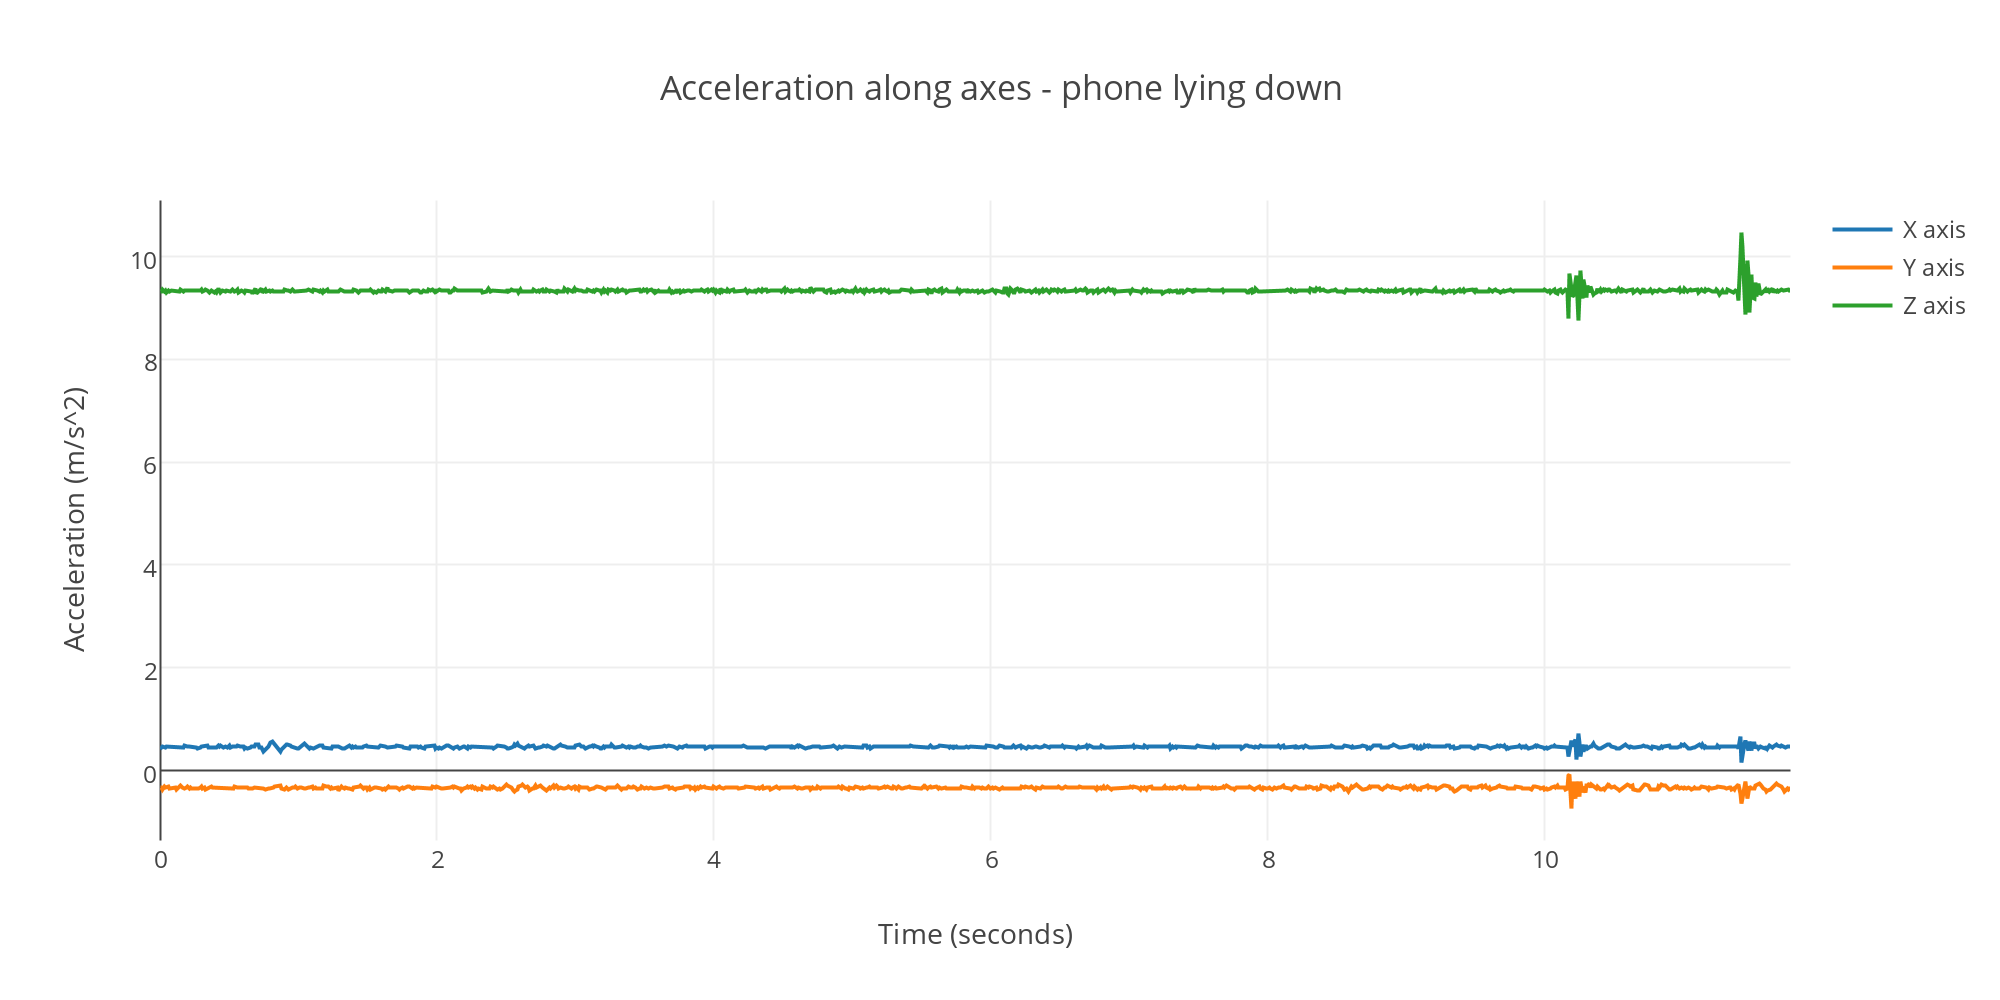
\includegraphics[scale=0.9]{images/accelerationZ.png}
\captionof{figure}{Accelerometer readings with phone kept flat on the surface}
\label{fig:accelerationZ}
\end{center}

As expected, the acceleration along the X and Y axes is close to 0, while there is a constant acceleration of about $9.81 m/s^2$ along the Z-axis due to the force of gravity acting downwards through the screen of the phone. Note that the direction of acceleration in this case is upwards as the phone at rest accelerates upwards with respect to the local reference frame of a freely falling object close to the surface. 

This process is repeated with the phone held upright this time (with the bottom of the phone in contact with the surface). The obtained readings are shown in Figure~\ref{fig:accelerationY}.

\begin{center}
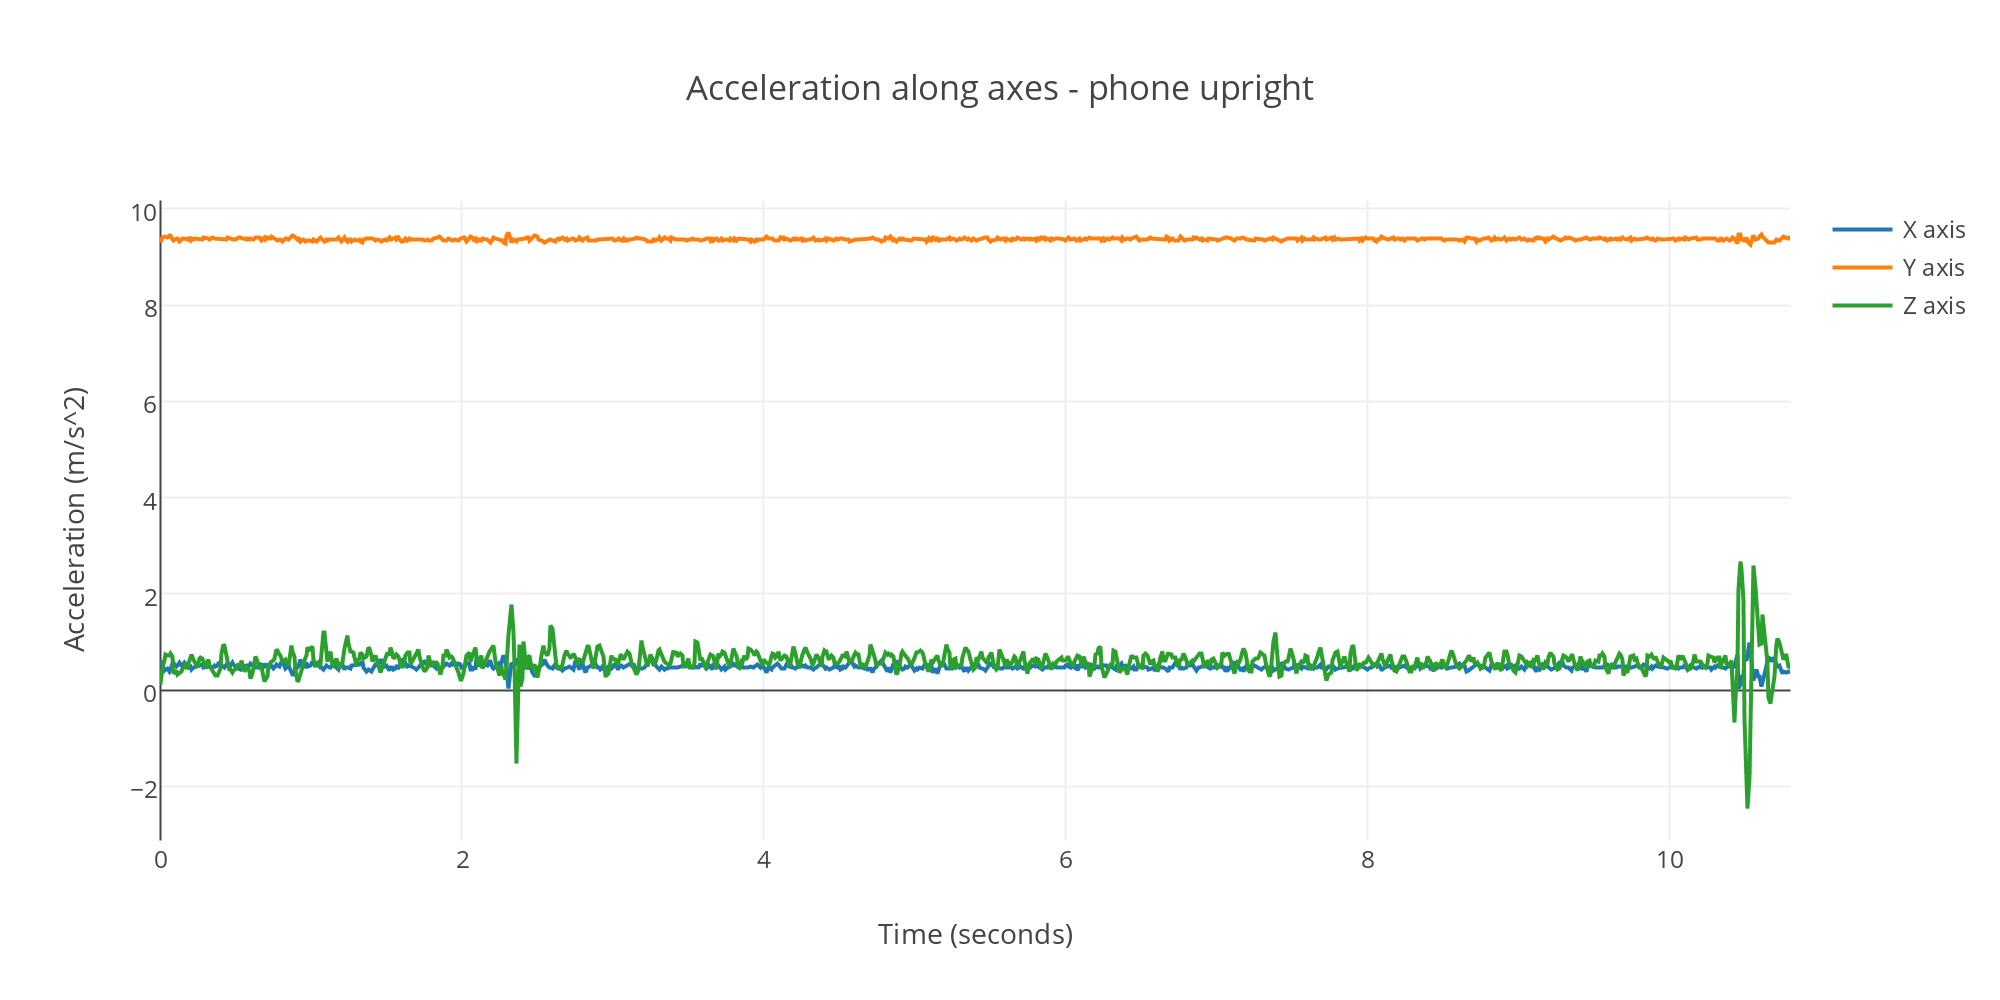
\includegraphics[scale=0.9]{images/accelerationY.png}
\captionof{figure}{Accelerometer readings with phone kept upright}
\label{fig:accelerationY}
\end{center}

The acceleration due to gravity is now along the Y-axis in accordance with the described behaviour, with the momentary spike in the Z-axis acceleration towards the end occurring due to slight movement of the hand while keeping the phone upright. On this basis it can also be concluded that keeping the phone lying on its side would make the gravity acceleration act along the X-axis, showing that the readings are consistent with the manner in which the phone's principal axes are defined. 
 
\subsubsection{Data Analysis}

After deciding that the accelerometer readings would form the basis of the step detection approach, the logging application was used to capture some acceleration data corresponding to walking motion to perform an initial analysis and detect any patterns that could be associated with individual steps. 

All data recording and subsequent step detection was done with the user holding the phone in-hand. Considering that step detection in this project is to be used in the context of a navigation system, the in-pocket case would only be useful to consider if our application was equipped to provide directional information in the form of audio updates, as the user would not be able to observe the phone's screen in this scenario. Our application provides navigation instructions in image and textual format only, in a similar vein to other applications such as Google Maps and hence the in-pocket case is not accounted for.  

The data was recorded while walking in a straight line for approximately 10 steps. 
The obtained data is depicted in Figure~\ref{fig:straightWalkRaw}. 

\begin{center}
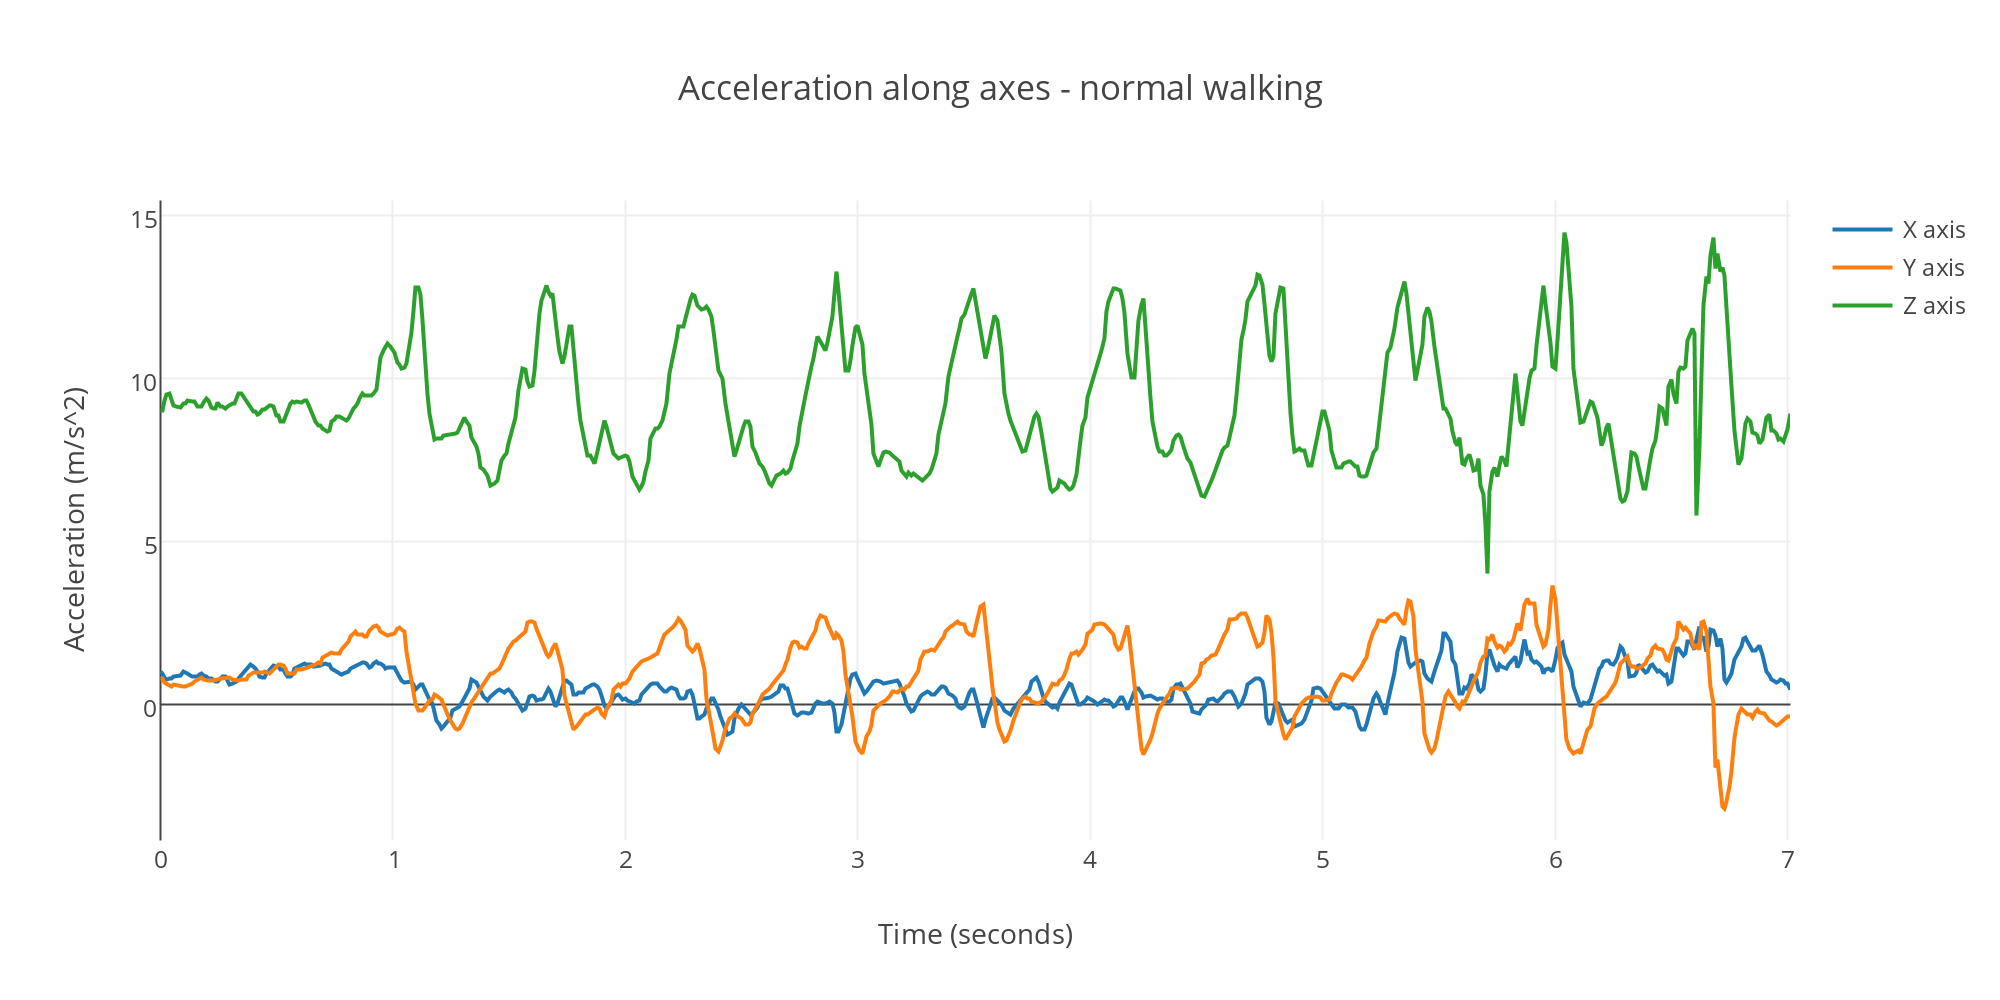
\includegraphics[scale=0.9]{images/straightWalkRaw.png}
\captionof{figure}{Accelerometer readings during normal walking}
\label{fig:straightWalkRaw}
\end{center}

As observed in the figure there is a periodic rise and fall in both the Y-axis and Z-axis accelerometer readings, while the X-axis readings do not exhibit much variation and remain close to 0 throughout. This is because when the phone is kept in the hand in portrait mode the majority of the gravity component is split vertically among the Y and Z axes, while there is negligible horizontal acceleration.

The periodicity in the Y and Z readings corresponds to the two phases of walking motion - the user beginning their step by lifting their foot off the surface followed by completing the step with bringing their foot down to make contact with the surface again. The first phase causes the phone to accelerate vertically along the direction of gravity acceleration as the user moves upwards. These are represented as peaks in the graph as the accelerations add together. In the second phase the user moves downwards and thus accelerates in a direction opposite to that of the gravity acceleration, leading to the formation of the valleys in the graph. Thus each peak/valley combination can be associated with individual steps, potentially allowing step identification to be carried out by detecting peaks and valleys in the graph generated by the accelerometer readings. This notion is supported by the plot in Figure~\ref{fig:straightWalkRaw}, where there are roughly 10 peak/valley pairs for both the Y and Z readings corresponding to the 10 steps taken.   

The primary issue with this approach is that step detection is dependent on the orientation in which the phone is kept. For instance, if the user holds the phone in landscape mode instead of portrait then a major component of the acceleration will  be along the X-axis. This makes it difficult to keep track of periodic changes in acceleration as variations along all the three axes must be considered simultaneously depending on the phone's orientation. This problem is overcome by computing the magnitude of the accelerometer vector and using that instead to detect steps. The magnitude combines the acceleration information from the three axes into a single scalar quantity, which by definition, is independent of direction and makes it robust to changes in orientation. The magnitude plot of the acceleration values in Figure~\ref{fig:straightWalkRaw} is provided in Figure~\ref{fig:straightWalkRawMagnitude}. 

\begin{center}
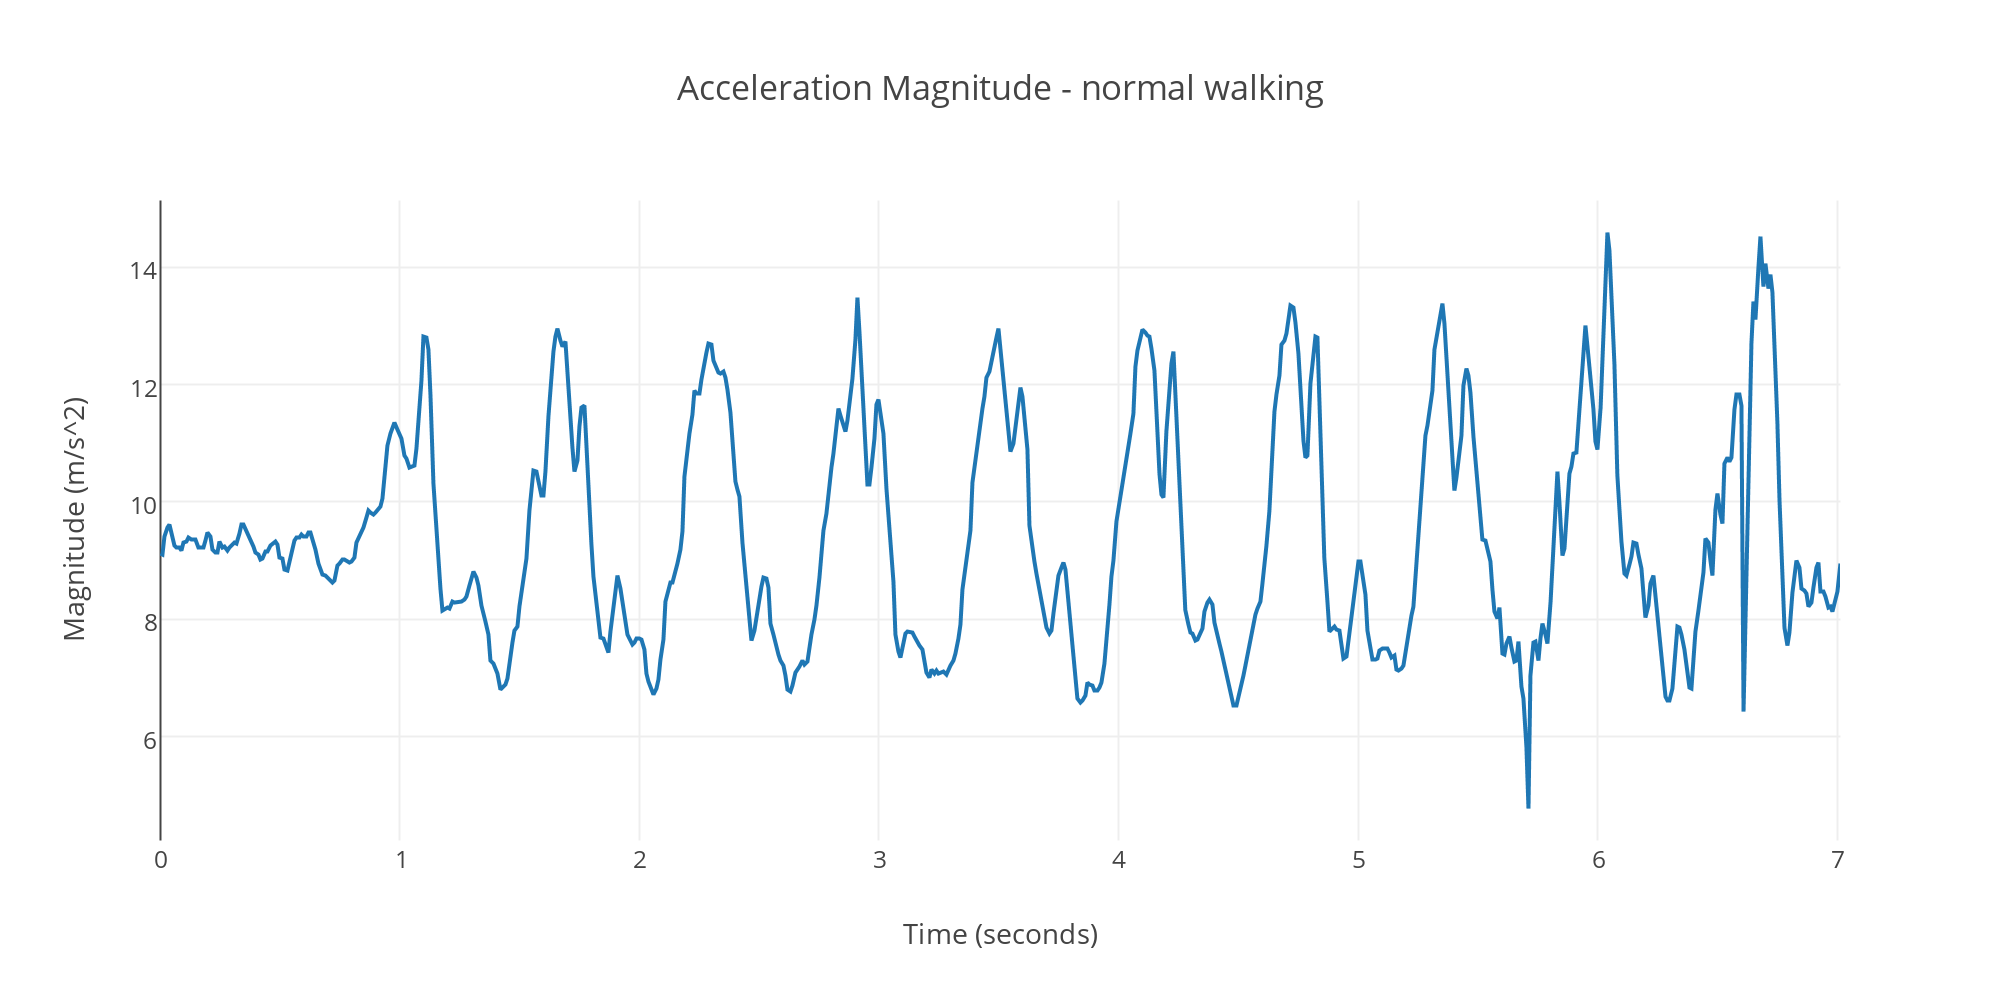
\includegraphics[scale=0.9]{images/straightWalkRawMagnitude.png}
\captionof{figure}{Accelerometer magnitude during normal walking}
\label{fig:straightWalkRawMagnitude}
\end{center}

From the plot it can be seen that using magnitude still preserves the 10 peak/valley pairs corresponding to steps that were identified in the previous graph. Thus step detection can now be carried out on the basis of a single measure that accounts for changes in orientation. 

\subsubsection{Peak/valley detection}

Figures~\ref{fig:straightWalkRaw} and~\ref{fig:straightWalkRawMagnitude} show a clear association between steps taken and peak/valley pairs in the graph. Thus individual steps can be identified by detecting the formation of such pairs in real-time. Mathematically, peaks are defined as points in the graph where the slope transitions from positive to negative. Equation~\ref{eq:peakDetection} shows how it can be determined whether a point is a peak. 

\begin{equation}\label{eq:peakDetection}
\begin{split}
previousSlope = a(n) - a(n-1) \\
newSlope = a(n+1) - a(n) \\
a(n) = peak\ if\ previousSlope > 0\ \&\ newSlope < 0
\end{split}
\end{equation}
where $a(n)$ is the $n$th reading from the accelerometer. Similarly, valleys are defined as points where the slope transitions from negative to positive. Equation~\ref{eq:valleyDetection} gives the criteria for a point to be classified as a valley. 

\begin{equation}\label{eq:valleyDetection}
a(n) = valley\ if\ previousSlope < 0\ \&\ newSlope > 0
\end{equation}
In the application, each new reading from the accelerometer is checked to see whether it is a peak or valley. This is done by maintaining a small sliding window of the three most recent accelerometer values. The middle value in this window is the one which is subject to the peak/valley check as the required slopes can be computed from the adjacent values. A step event is thus fired whenever a valley and peak are detected in succession.  

On applying this step detection approach to the graph in Figure~\ref{fig:straightWalkRawMagnitude} it is found that the number steps returned by the algorithm is significantly greater than the actual number of steps that were taken. This is due to the jagged nature of the graph, which is a consequence of the phone's accelerometer having high sensitivity. Even very slight movements cause non-negligible acceleration to be recorded, which leads to the introduction of a considerable amount of noise arising from the jitters and vibrations experienced by the phone while walking. These jitters result in a number of small kinks in the accelerometer graph that are interpreted as peaks/valleys by the step detector, triggering false positives. There is thus a need to remove these kinks by applying some smoothing so that only large changes in acceleration cause peaks and valleys to be formed.  

\subsubsection{Barometer}

For the barometer, both Andriod and iOS have native ways to get both the current air pressure and the height above sea level the device. From research and small amounts of testing it was evident that using the absolute height would not provide any useful way of detecting floor change with the fluctuations that occur with time, weather and location. To avoid this the difference between heights can be used to detect if a user has gone up or down a floor. 

However despite there being a clear correlation between moving between floors and the change in height, the height recieved from these native functions would range between 3-5m over a small period of time. This means that it is very difficult to be certain if the user has changed floors, the difference in floor height with in the department is 4m, or it is simply an outlier from the functions. 

To help combat this the average was taken over a large number of reading across a period of time, however whilst this solved the rapidly changing value, it meant that if a user took too long transistioning between floors the average would slowly slide in their direction of movement. When this occurs nothing will be flagged as a large enough distance to be moving from floor A to B and the system will not recognise the movement. 

Given more time this issues could be solved, and from research and the testing done it can be seen that the barometer will be a useful sensor for indoor localisation.

\subsubsection{Landmarks}

Before implementing a system that uses landmarks, the options for potential landmarks first have to be analysed as to whether they can provide the benefits in our specific environment. The main options that were explored are:

\begin{itemize}
	\item Stairs
	\item Elevators
	\item Areas of unique magnetic readings
	\item Wi-fi Routers
\end{itemize}

The first 2 options are present in the department building, however they are limited in how they can help with resetting the error in the system. This is because stairs and elevators are naturally only used when moving from one floor to another. Meaning navigation on a single floor will not be helped with resetting error but for navigation over multiple floors they can be utilised. 

Both have unique patterns that can be seen from the accelerometer readings, in conjunction with the potential for the barometer to verify the movement between floors, they can be used as landmarks. However a detection algorithm did not get implemented for either of the patterns, to still allow for the removal of error build up the user is requested to alert the application when they have moved from one floor to another.

Magnetic readings are likely to be prevelant throughout our environment as the entire building has lots of electronic equipment, such as computers, servers, etc.... These readings manifest themselves more in general magnetic inteference as appose to small pockets of unique signals, this makes areas of magnetic readings unfeasible as a landmark in our scenario.

This leaves Wi-fi as the only method of removing error when navigating within a floor, to do this all the routers on a floor need to be identified.

\begin{center}
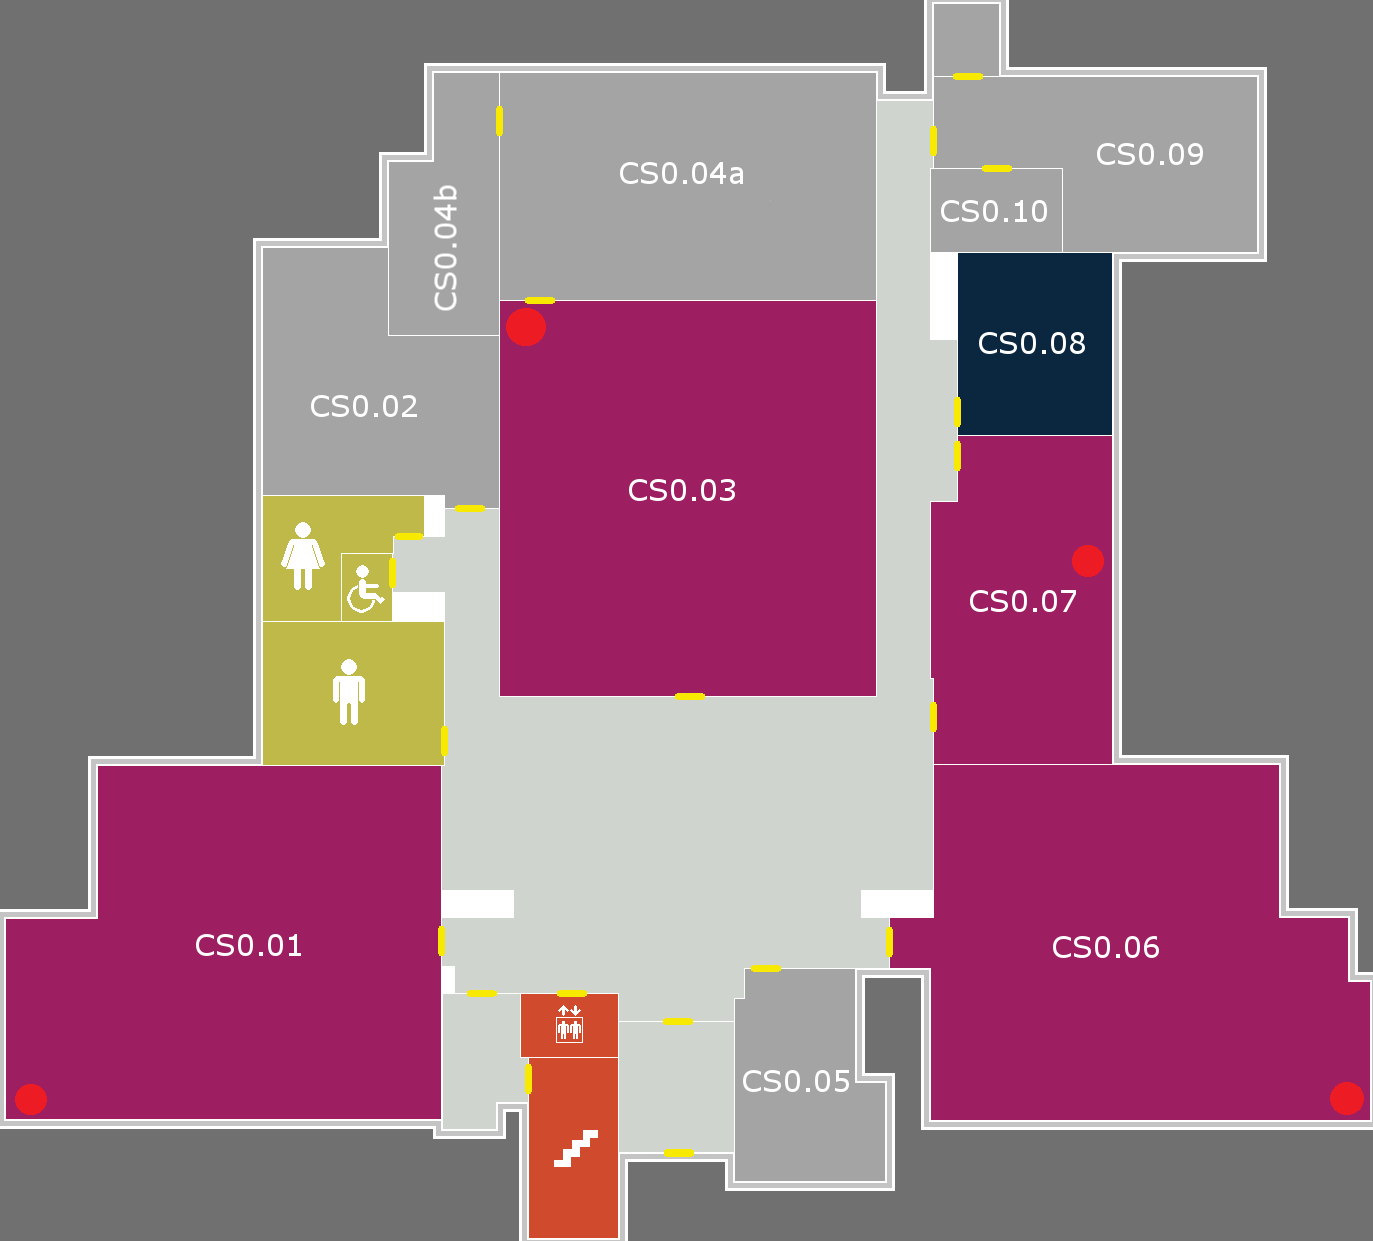
\includegraphics[scale=0.3]{images-implementation/wifiLocation.png}
\captionof{figure}{The location of Wifi routers on the ground floor of DCS, marked as red dots}
\label{fig:wifiLoc}
\end{center}

After identifying the locations of the routers on the ground floor, as shown in Figure~\ref{fig:wifiLoc}, it becomes apparent that bar one they will not be able to serve as landmarks. They reside with in the corners/sides of the rooms, and for a landmark to be useful the user must path close enough to it for it to be a viable choice for resetting error. With most of their locations it is impossible for an effecient routing algorithm to return a path in which the routers are not either at the start or the end of the route. Hence making them effectively useless for this purpose. The singular router that could be used is the one residing within CS0.03, as it sits before a door that leads to two other rooms. Despite this ideal placement it still isn't suited for use as a Landmark, as the two rooms for which the pathing would make the user pass by the router have restricted access due to containing servers/equipment.

We also found that we often picked up routers from different floors in certian areas, whilst this could be a landmark in a similar way to pockets of magnetic readings. It was not consistent across different devices used for testing, hence not viable for a landmark since it isn't available to all. As well as this devices would connect to a room's router outside of them, meaning that connecting to a router that is specific to a large room it is an unreliable to assume the user is within it.

Whilst routers are not viable for landmarks on the ground floor for the reasons stated above, it doesn't mean they will not be viable for the upper floors. This was tested the same as before by identifying router locations, but it became quickly evident that from placement again they would not be of use. In conjunction with the large number of small rooms/offices on the upper floors it becomes hard to snap a user to these routers.

Another thing to note about using routers is that there are two main bands that are used for communication, 2Ghz and 5Ghz, so dependent on the routers and smartphones they may not be usable. In this case the router's in the department are dualband meaning both are available, it does however mean that 2 MAC addresses are needed to be stored per router for unique identification.

Overall having looked at these landmarks it is clear that all of these options could be useful in the right environment, unfortunately in our case a variety of factors play a role in making them infeasible.

\chapter{Proposed Solution}

Considering the research conducted thus far, the existing solutions that were analysed and the objectives set at the onset of the project, we propose the following solution.

\paragraph{Dead Reckoning Based On Step Detection}

: We propose the use of a step detection algrotihm that tracks a user's movement based on the readings of the inertial sensors of a smarthphone. In a dead-reckoning system, a user's current position is determined by incrementally estimating their displacement from a previously known position. Thus if the user's starting location is known, step detection along with the user's bearing can be used to identify when they have moved and along which direction. Our desire to create an infrastructureless application made the use of other techniques unattractive, with the prevalence of step detection within existing solutions also indicating that step detection is a productive avenue of development.

\paragraph{Heading Based on Compass Readings}

: Compass readings indicate the current heading of the smartphone. Considering that the smartphone will be held by the user and face the direction of travel, this heading can also be inferred as being the direction of the user.

\paragraph{Pathfinding and Wall Collision}
: This is a unique concept not featured in any of the existing solutions that we examined. It involves the use of pathfinding algorithms to create routes within buildings, with wall collision used to correct erroneous user movement. 

\section{System Overview}

\subsection{Preprocessing}

The pathfinding and wall collision components of the application require preprocessing to occur on the floor plan images of buildings. The preprocessing diagram depicted ~\ref{fig:preFlow} is tailored to the specific requirements of the University of Warwick computer science department floor plans.

\begin{figure}[h]
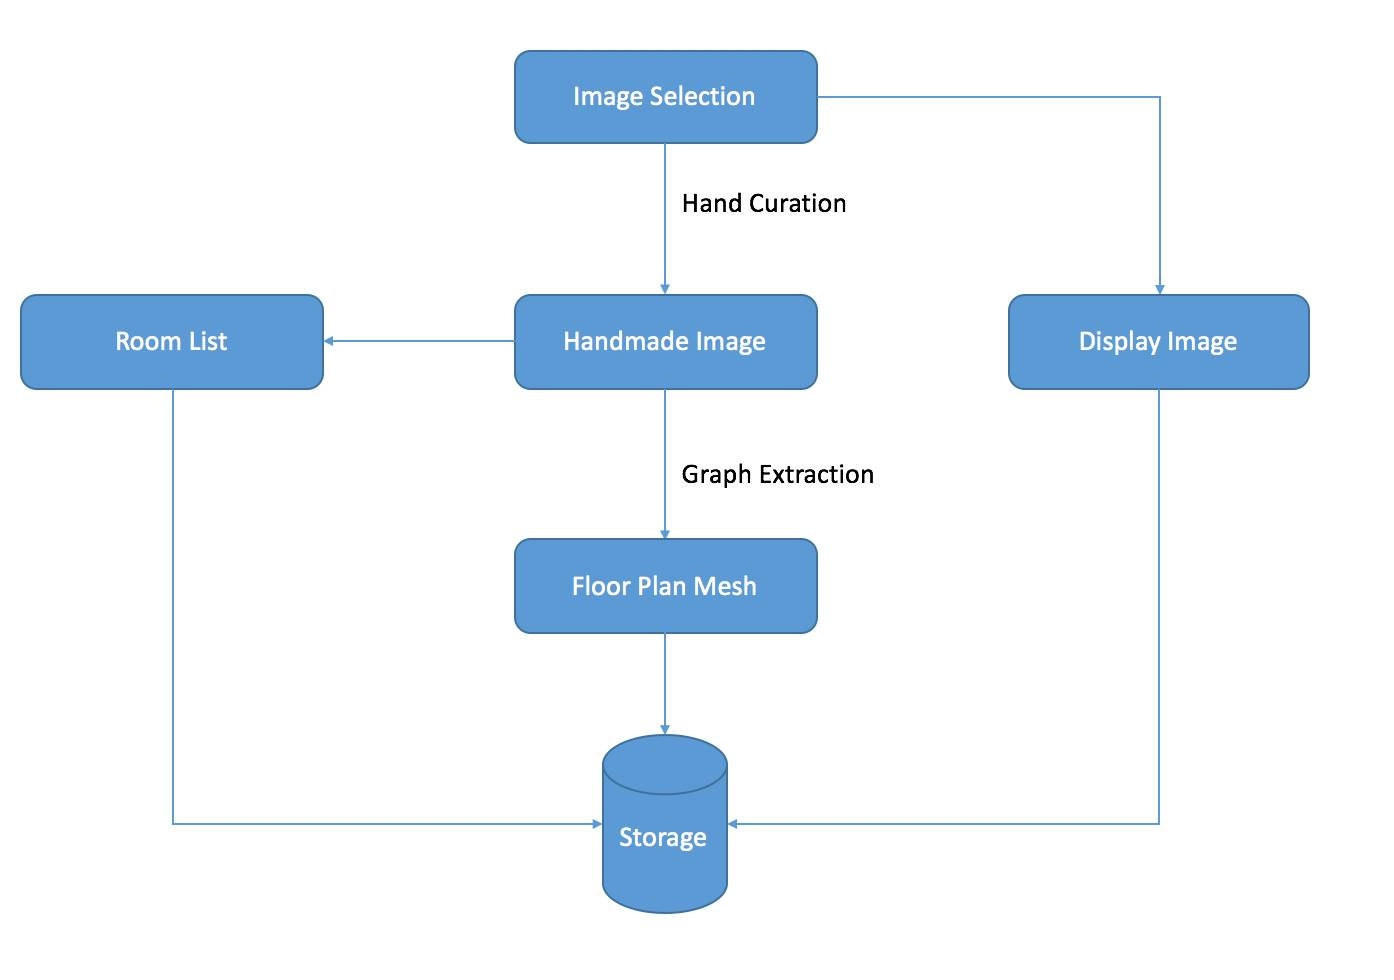
\includegraphics[width=\textwidth]{images/preFlow.png}
\captionof{figure}{Application preprocessing flow diagram.}
\label{fig:preFlow}
\end{figure}

\paragraph{Image Selection}
Images are obtained from the University of Warwick's online interactive map, which provides floor plan images of all the University's buildings.

\paragraph{Hand Made Image}
In order for these images to be processed, these need to be hand curated and made into the required format.

\paragraph{Graph Extration}
In order to have a graph from which to implement path finding, an adapted flood fill algorithm is used on the hand curated floor plan. This creates a mesh of all accessible areas within a floor, omitting links that would cross walls or enter areas outside of the bounds of the floor plan.

\paragraph{Room List}
This is a collection of rooms contained within a building. Each entry comprises the room's name and associated metadata which stores the rooms properties, such as position, occupier, floor etc.

\paragraph{Display Image}
This is the finalised image of the floor plan that will be displayed to the user.

\subsection{Application}
Once the preprocessing is accomplished, this is stored and used by the main application. The application flow diagram is shown within figure ~\ref{fig:appFlow}.

\begin{figure}[h]
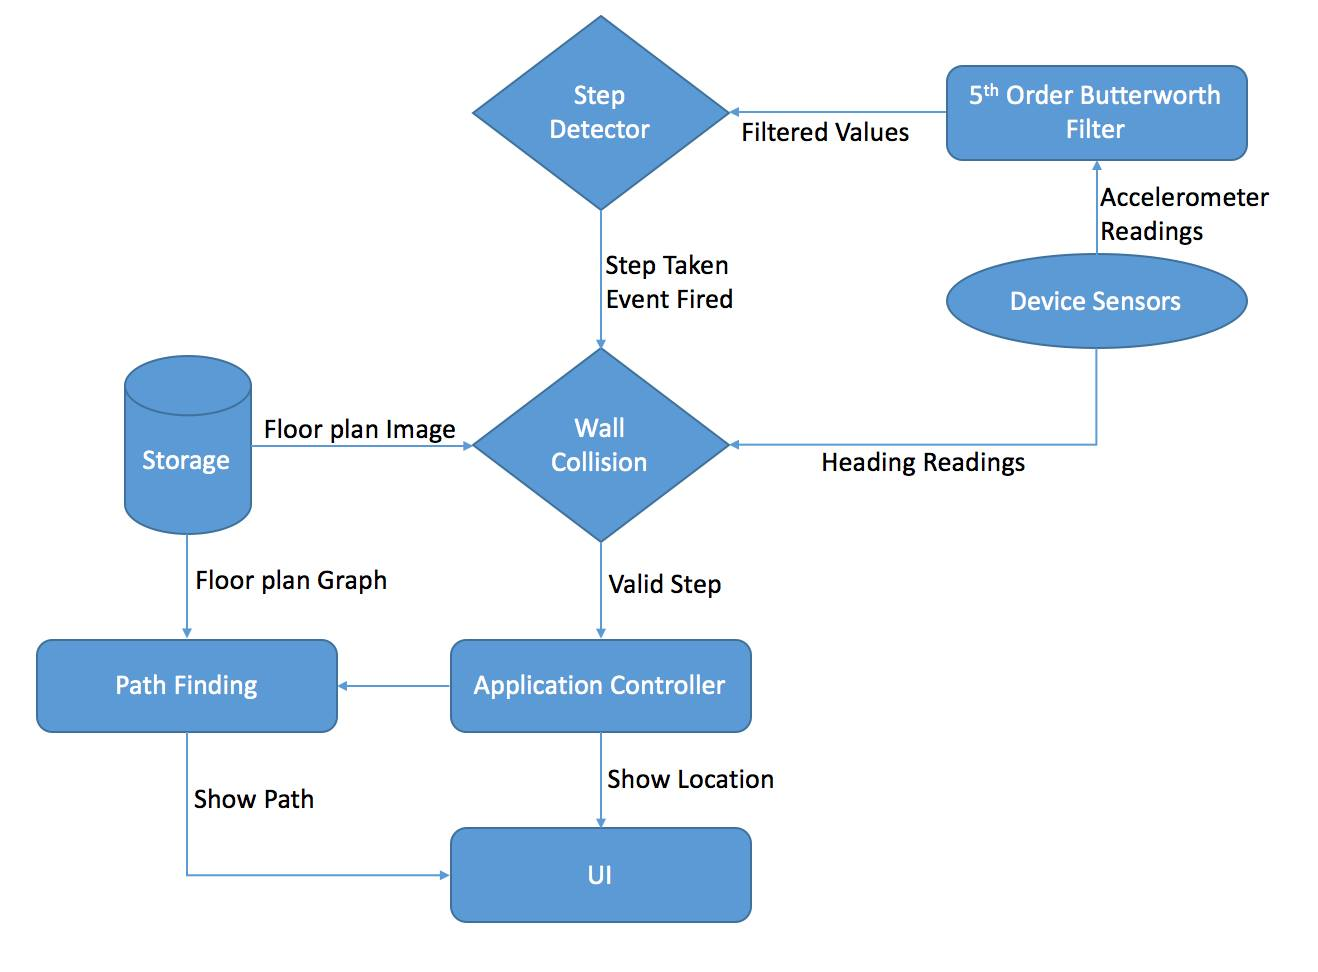
\includegraphics[width=\textwidth]{images/appFlow.png}
\captionof{figure}{Main application flow diagram.}
\label{fig:appFlow}
\end{figure}

\paragraph{Sensors}
The accelereometer and magnetometer are the primary sensors of use. These sensors are subscribed to as events and provide updated information for the rest of the application every 10ms.

\paragraph{Butterworth Filter}
The accelerometer values are very noisy and require filtering before use by the step detection system. A 5th order Butterworth filter is used for this process, as it provides the optimal balance between responsiveness, accuracy and robustness.

\paragraph{Step Detector}
The step detector takes the filtered accelerometer values and analyses the fluctuations produced by standard walking motion. Occurences of peak and valley pairs fulfilling certain criteria represent individual steps.

\paragraph{Wall Collision}
Makes use of native Android and iOS functions in order to access the image data of the hand curated floor plan. Within these floor plans, only inaccessible areas such as walls are represented in white. The wall collision system checks that any step will not cause the user to walk through, or land on, any inaccessible area, by checking whether a line cast between the source and end point passes over any white pixel.

\paragraph{Path Finding}
Makes use of the extracted graphs to find the shortest path between a source and end node, in manhattan distance. Path finding makes use of Dijkstras algorithm, which exploits caching and allows for faster turnaround times.

\chapter{Algorithm Design}

\section{Step Detection Algorithm}

\subsection{Low-pass filtering}

A low-pass filter is one which allows low frequency signals to pass through while attenuating signals that are above a defined `cut-off frequency'. In essence, it smooths the signal by eliminating small, momentary fluctuations while preserving any significant changes in the signal that occur gradually over a longer period. Hence a low-pass filter is applied to the accelerometer readings in order to counteract the effects of the added noise and remove the kinks in the graph which contribute to false positives, while resulting in the peaks and valleys corresponding to steps taken to be more well defined. 

\subsubsection{Exponential smoothing}

The simplest type of low-pass filter is a first-order one. The order of a filter refers to how sharply it reduces the amplitude of a signal whenever its frequency doubles. For instance, a first-order filter halves the signal's amplitude while higher orders cause greater reductions~\cite[p.2528]{casiez20121}. A simple digital implementation of a first-order low-pass filter is given in Equation~\ref{eq:lowPass}.   

\begin{equation}\label{eq:lowPass}
\hat{a}(n) = \alpha \times a(n) + (1 - \alpha) \times \hat{a}(n-1)
\end{equation}
where $\hat{a}(n)$ is the $n$th filtered accelerometer value, and $\alpha$ is a constant, known as the smoothing factor, between 0 and 1. Lower values of $\alpha$ (say 0.25) mean that each new filtered value is computed by taking a large proportion of the previous filter output and providing a slight update to it using the most recent raw accelerometer reading. This is represented diagrammatically in Figure~\ref{fig:complementaryFilter}.  

\begin{center}
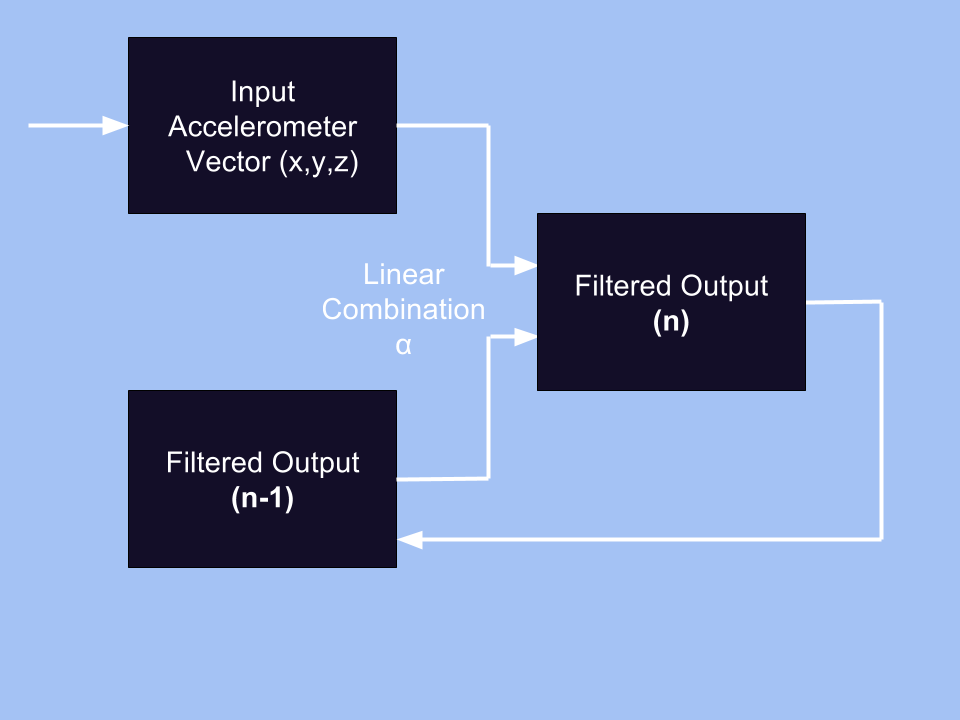
\includegraphics[scale=0.3]{images/complementaryFilter.png}
\captionof{figure}{First order low-pass filter for accelerometer readings}
\label{fig:complementaryFilter}
\end{center}
Thus any variations in the raw input values must occur consistently over a sustained time period for it to be reflected in the filtered output. This process is known as `exponential smoothing' since ``the contribution of the older values exponentially decreases'' over time~\cite[p.2528]{casiez20121}. The result of applying this filter on the magnitude values in Figure~\ref{fig:straightWalkRawMagnitude} is shown in Figure~\ref{fig:complementaryFilterMagnitude}. 

\begin{center}
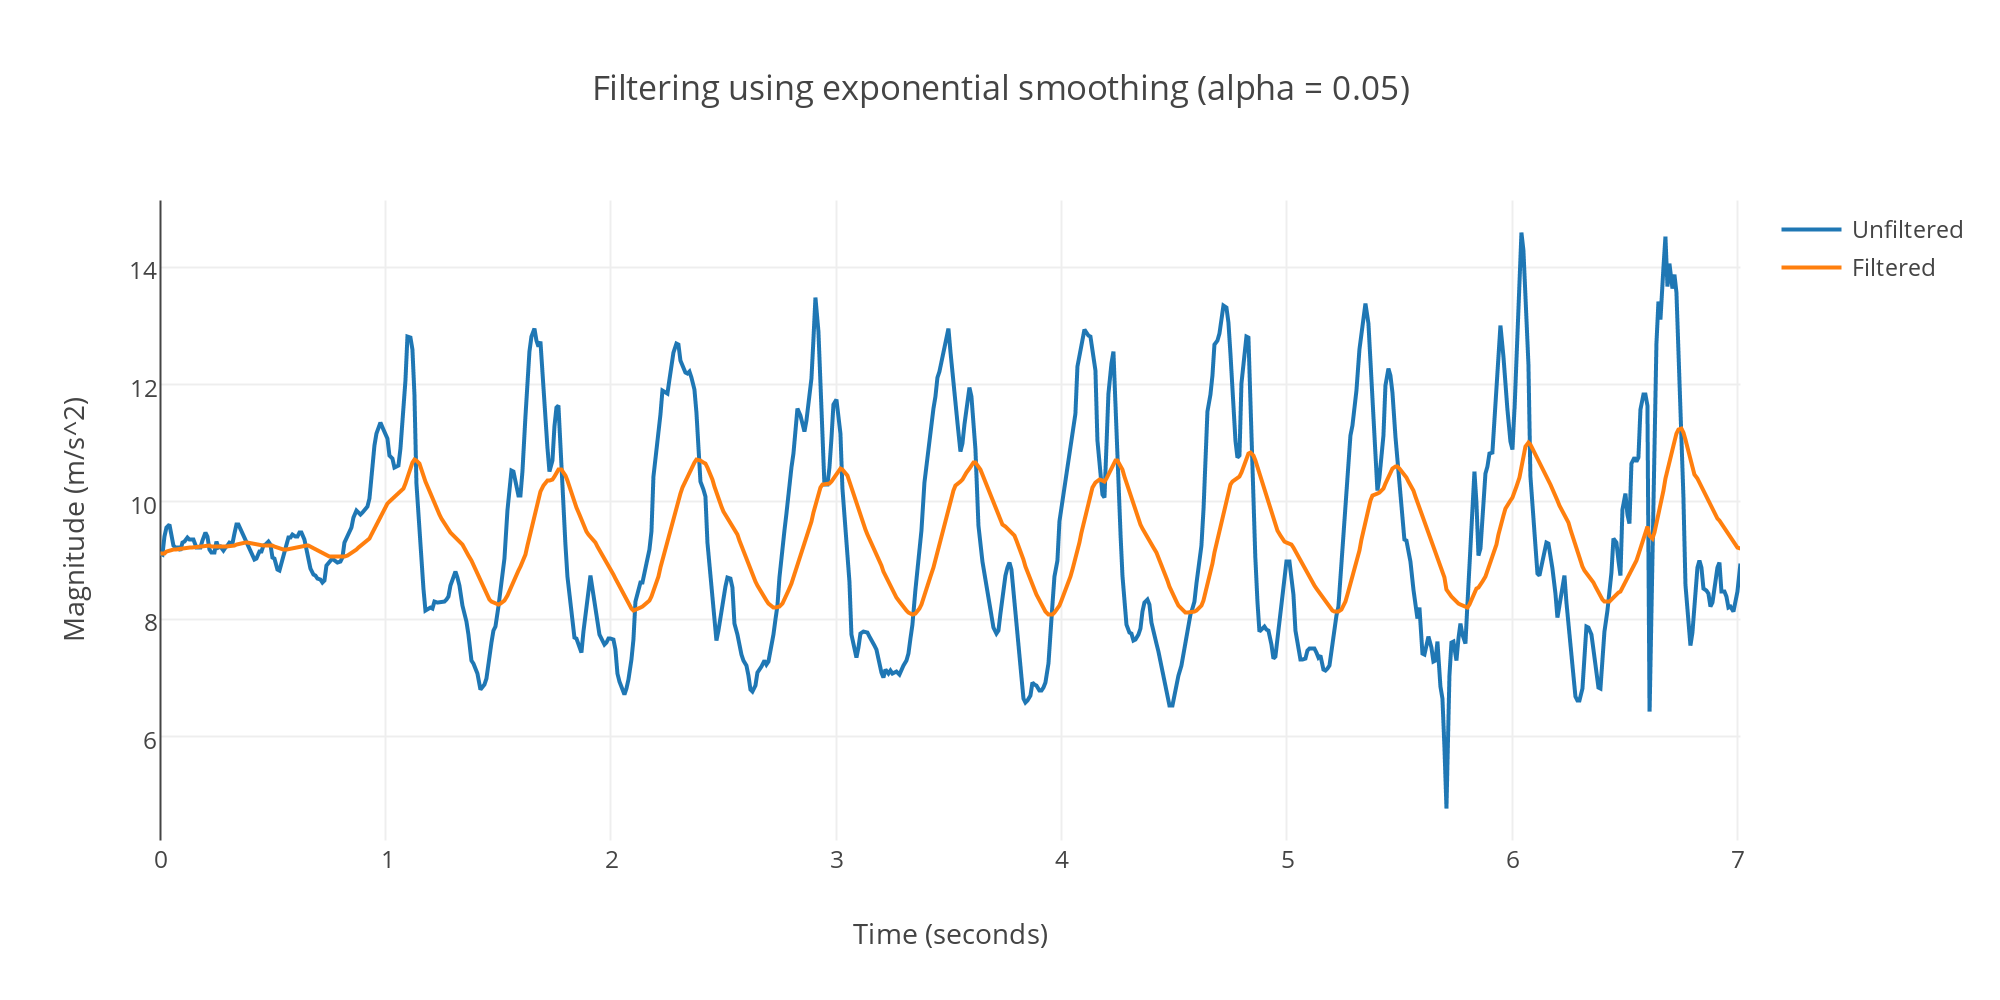
\includegraphics[scale=0.9]{images/complementaryFilterMagnitude.png}
\captionof{figure}{Result of applying exponential smoothing to the unfiltered magnitude}
\label{fig:complementaryFilterMagnitude}
\end{center}

The filtered graph obtained is far smoother than its unfiltered counterpart and removes most of its kinks, thus reducing the number of false positives with regards to step detection.   

On initial tests using this approach the step counting was found to be fairly accurate during standard walking motion, with each individual step being detected almost immediately after it was actually taken. However, step events were also often found to fire when the user was stationary and performing other activities while having the phone in their hand. For instance, it was observed that modest hand motions of the user while standing and talking to someone resulted in steps being recorded. This suggests that the accelerometer magnitude patterns produced by such motions are similar to those obtained while walking. In order to investigate this the logging application was used to record accelerometer values while the phone was kept in hand and moved up and down slightly in a periodic manner without taking any steps. The filtered output from this recording is shown in Figure~\ref{fig:complementaryFilterHandMotionMagnitude}. 

\begin{center}
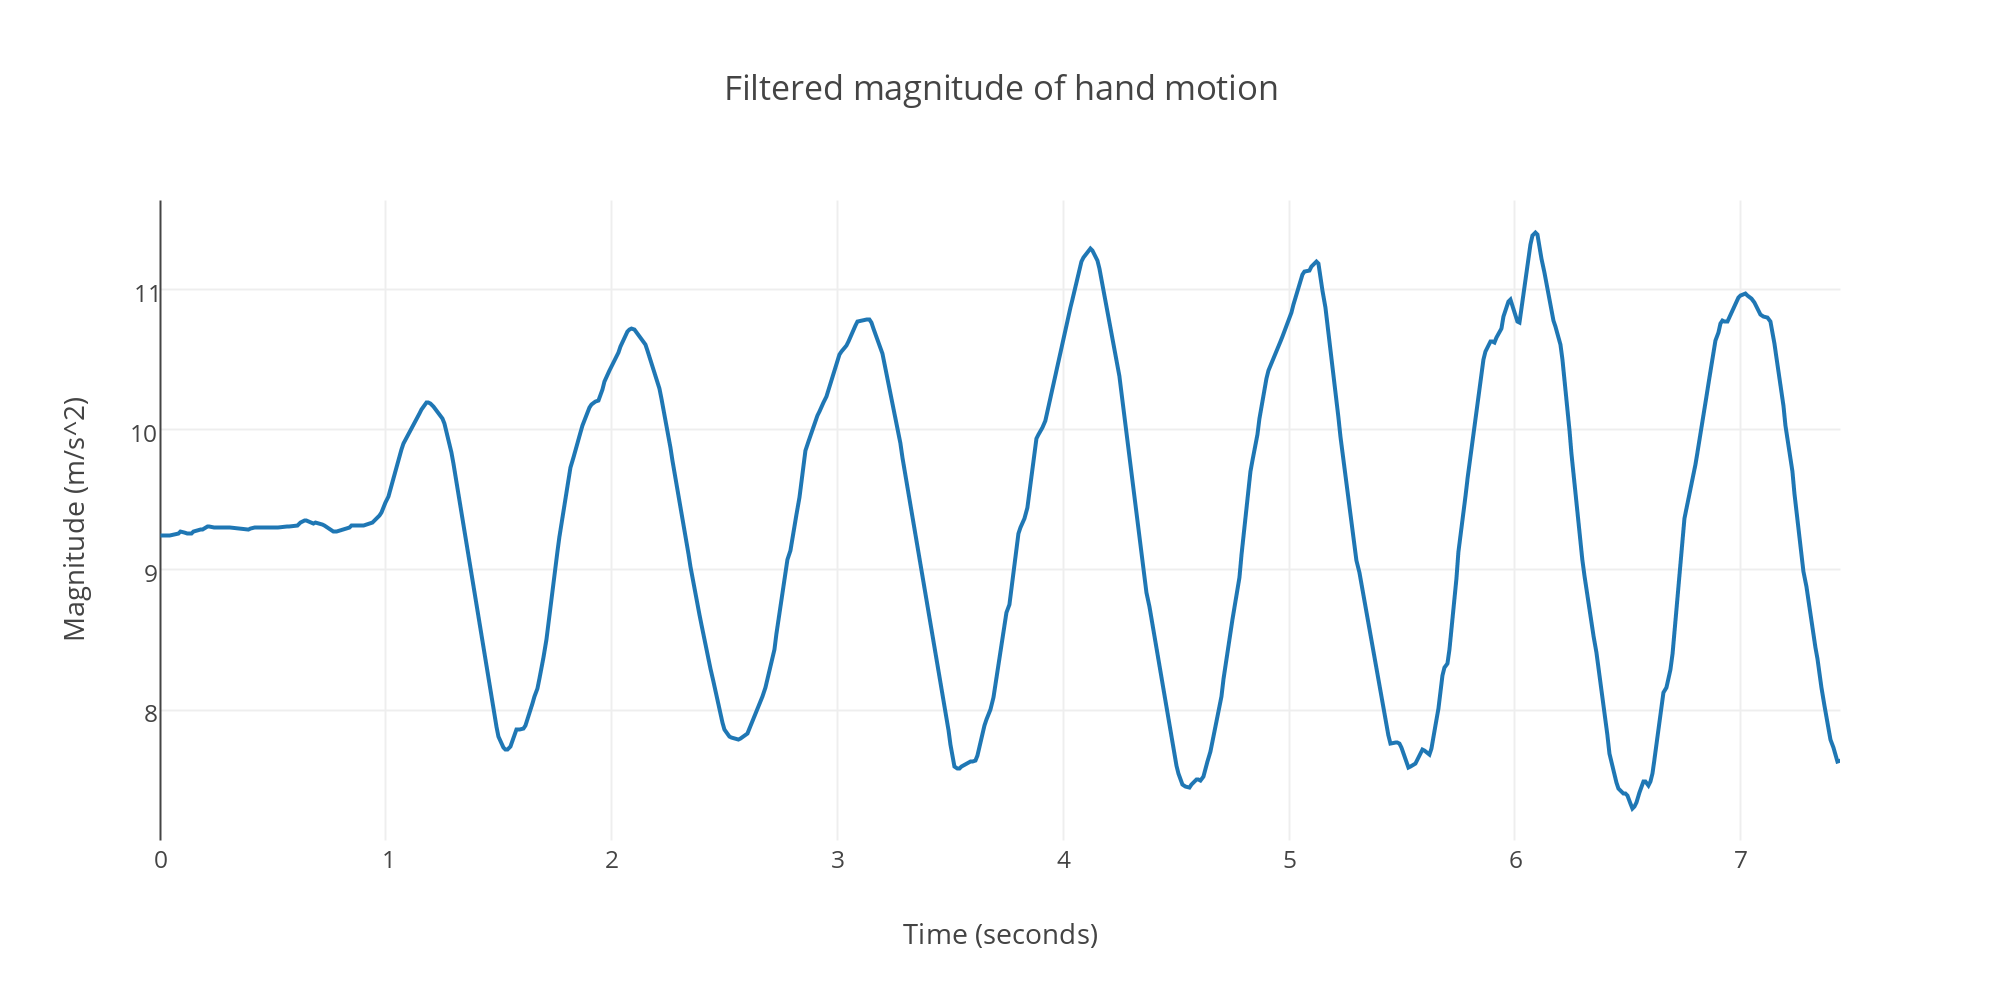
\includegraphics[scale=0.9]{images/complementaryFilterHandMotionMagnitude.png}
\captionof{figure}{Filtered magnitude of hand motion}
\label{fig:complementaryFilterHandMotionMagnitude}
\end{center}
The plot confirms that using the exponential smoothing method to filter these hand motions produces peak/valley combinations that are almost indistinguishable from normal walking motion and results in steps being detected falsely. This first-order filter is thus deemed to be too sensitive for the purpose of navigation. 

\subsubsection{Butterworth Filter}

A `Butterworth' low-pass filter is one that is mathematically designed to provide as flat a frequency response as possible in the passband while dropping off towards zero in the stopband~\cite[p.17]{bianchi2007electronic}. This means that in the ideal scenario, components of the signal below the cut-off frequency are passed through at maximum amplitude without any ripples while high frequency components are eliminated through attenuation. This is depicted in Figure~\ref{fig:butterworthResponse}.   

\begin{center}
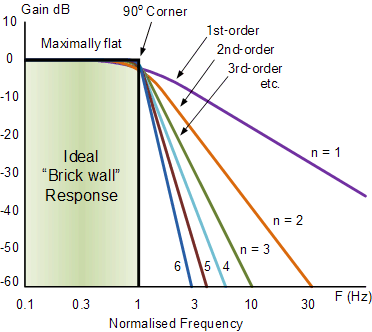
\includegraphics[scale=0.9]{images/butterworthResponse.png}
\captionof{figure}{Plot of gain vs normalised frequency for various Butterworth filter orders~\cite{butterworthResponse}}
\label{fig:butterworthResponse}
\end{center}
The `brick wall' response represents the ideal case with the steepest possible 90 degree corner passband, where the amplitude of any signal greater than the cut-off frequency immediately drops to zero. For practical purposes however, it is only possible to obtain approximations for this ideal Butterworth response as maximal steepness produces significant passband ripple~\cite{butterworthResponse}. 

Using an approximation of this ideal response means that a flat passband can be achieved only by introducing a `transition band', the range of frequencies between the passband and stopband for which the amplitude is neither maximum nor zero. From the figure it can be seen that first-order filters have a very wide transition band, meaning that only signals that have considerably greater frequency than the cut-off are fully attenuated. Filters of greater order cause more aggressive attenuation, which is why increasing the order of the Butterworth filter leads to a better approximation of the ideal response as shown in the diagram. Thus using a high order Butterworth filter provides good separation between the passband and stopband while minimising the interference caused to the signal in the passband due to ripples.    

Mathie, M. analysed the manner in which readings from a triaxial accelerometer could be used to detect and classify a wide variety of human movements and actions. As part of this research, they found that the frequency range of 0.7-3 Hz encompasses most people's normal walking motions~\cite[p.248]{walkingFrequency}. This is derived from the total number of steps usually taken per minute while walking. Hence using a low-pass Butterworth filter with a 3 Hz cut-off frequency would allow isolation of the accelerometer signals associated with walking motion while removing any potential higher frequency components introduced by noise and other external factors. For instance, Susi, M., et al. employ a tenth-order Butterworth filter for pre-processing the accelerometer readings to make their step detection algorithm robust to such high frequency signals~\cite[p.1552]{susi2013motion}.  

With this in mind, we too tried using the same tenth-order Butterworth filter in order to see whether it would improve step detection performance in comparison to the first-order exponential smoothing approach. This filter was implemented by using an online tool provided by Fisher, T., a professor at the University of York~\cite{filterTool}, which takes user specified input parameters such as the desired cut-off frequency and filter order to generate the corresponding recursive Butterworth filter equation. The 3 Hz, tenth-order filter obtained computes each new filtered value on the basis of the 11 latest raw input values and 10 previous filter output values. The results of applying this filter on the normal walking and hand motion accelerometer readings are depicted in Figure~\ref{fig:butterworth10thOrderFilter}. 
\begin{center}
  \begin{minipage}[b]{0.5\textwidth}
    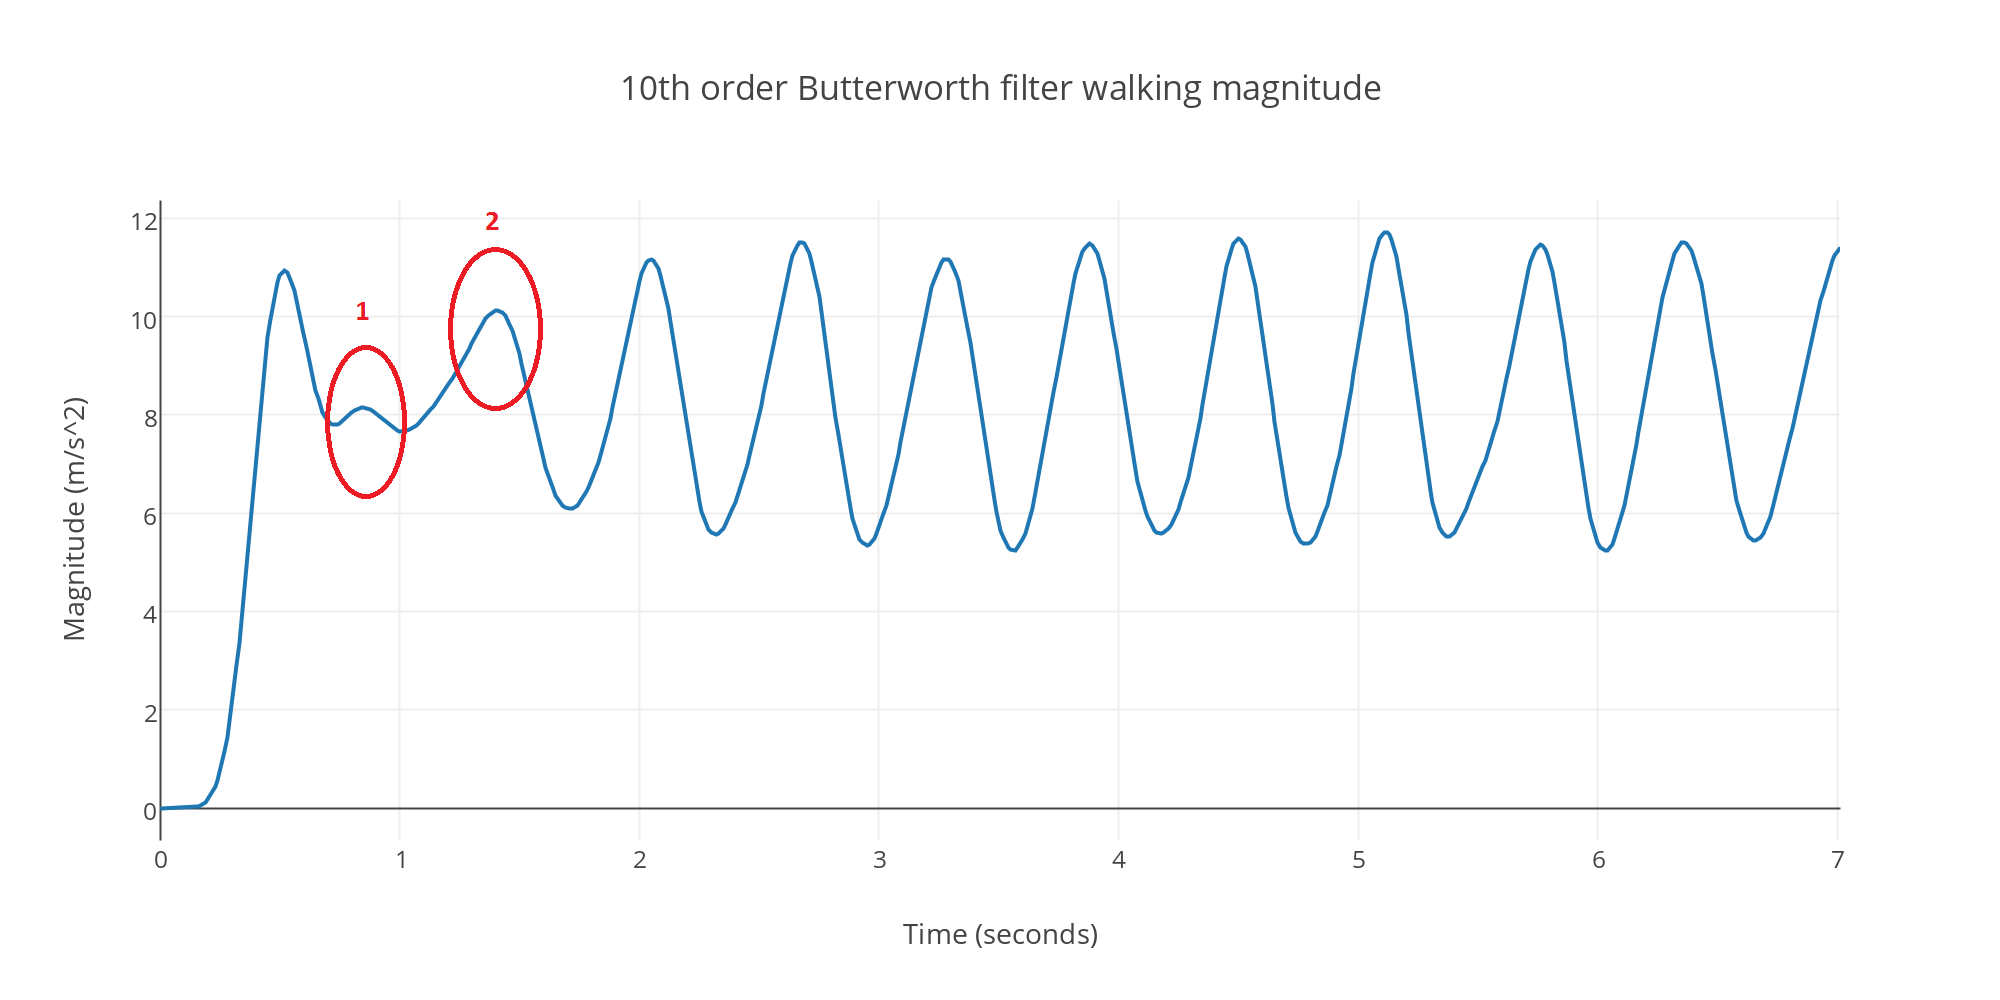
\includegraphics[scale=0.2]{images/butterworth10thOrderFilterWalkingMagnitude.png}
  \end{minipage}%
  \begin{minipage}[b]{0.5\textwidth}
    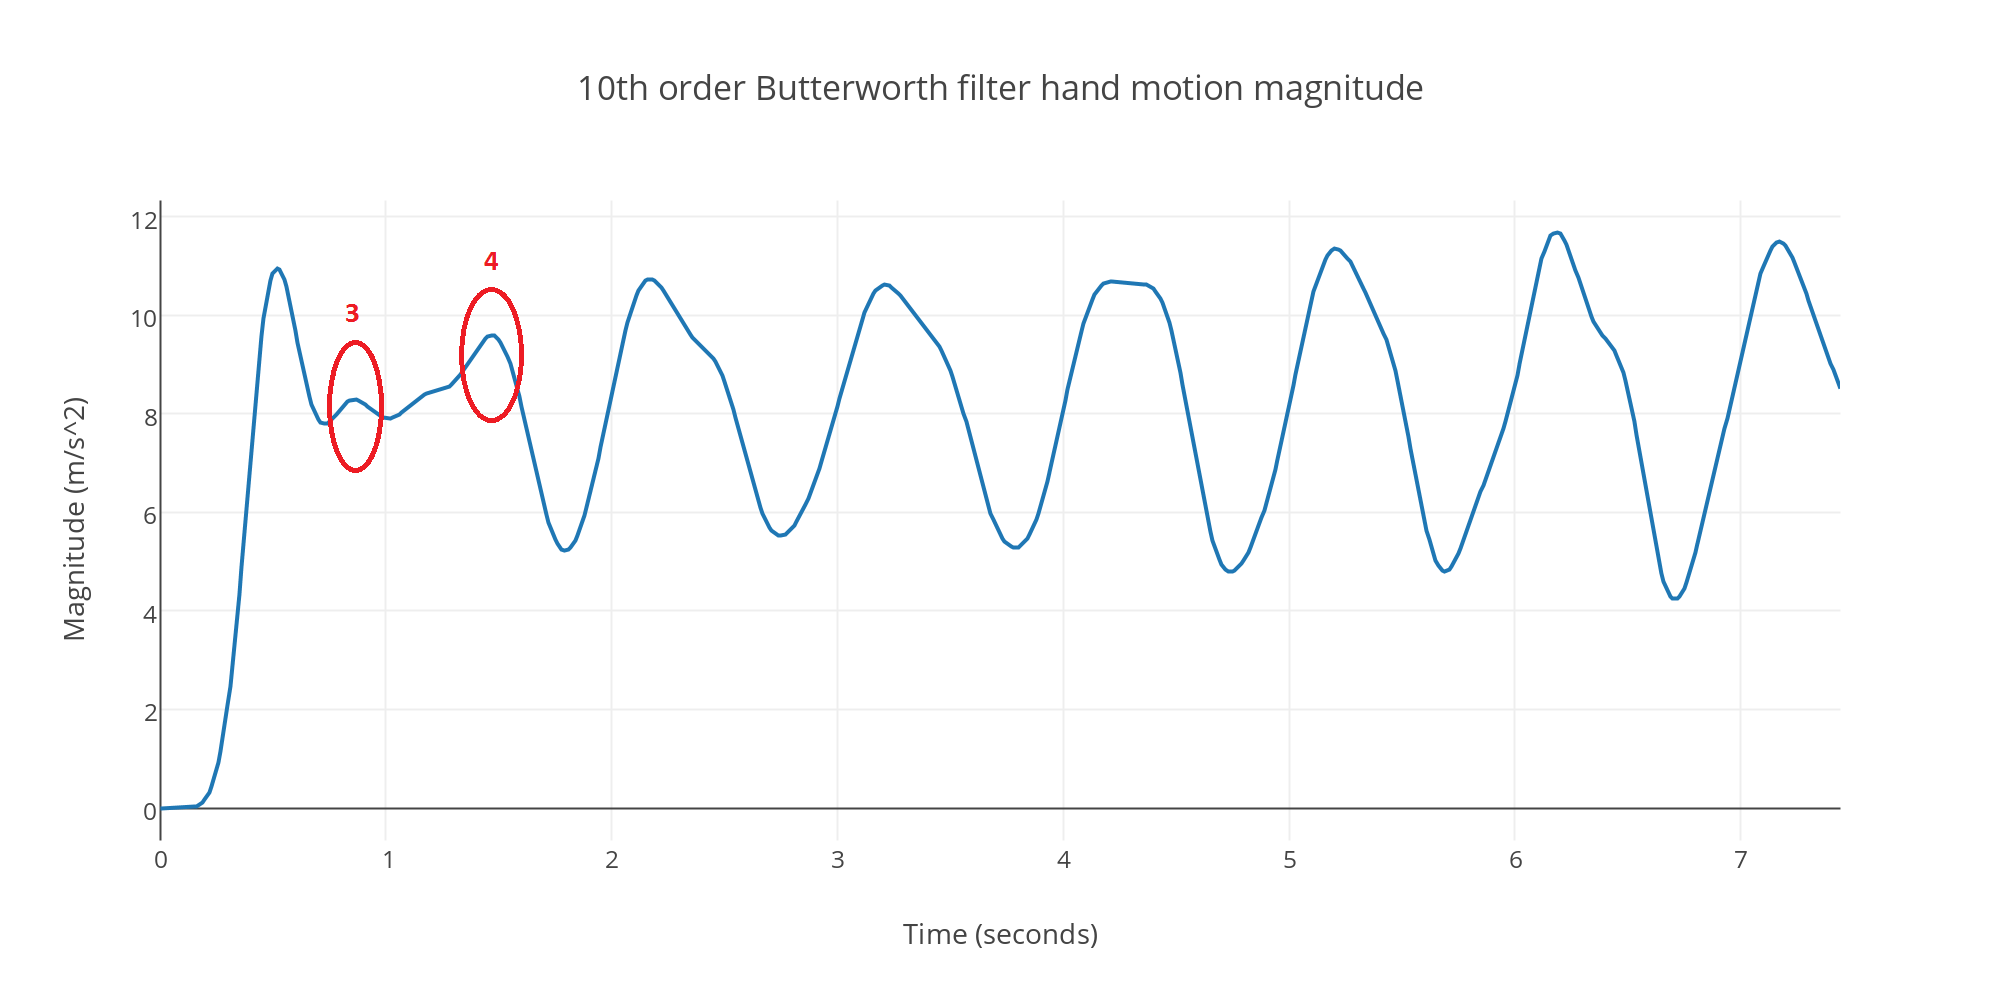
\includegraphics[scale=0.2]{images/butterworth10thOrderFilterHandMotionMagnitude.png}
\end{minipage}
\captionof{figure}{Results of applying the tenth-order Butterworth filter}
\label{fig:butterworth10thOrderFilter}
\end{center}
On initial inspection it seems that the filtered graphs obtained for both walking and hand motion are once again similar, just like they were for the first-order filter. However, there exists a significant difference between the two filters with regards to the magnitudes of the peaks/valleys obtained. In both the plots in Figure~\ref{fig:butterworth10thOrderFilter} the first peak is formed due to the initial adjustment of the filter as it shifts from its initial value of zero to the new magnitude values coming in, and hence this peak can be ignored for the purpose of step detection. The following two peaks in each plot, denoted by the numbers 1/2 and 3/4 respectively, have magnitude values that are noticeably lower than those of the subsequent peaks. Furthermore, the magnitude values of these subsequent peaks and valleys are largely consistent, that is, the peaks and valleys occur at almost the same magnitude values in all cases. Thus there is a clear differentiation between the first two peaks and the following ones. This is in contrast to the plots obtained when using the first-order filter (Figures~\ref{fig:complementaryFilterMagnitude} and~\ref{fig:complementaryFilterHandMotionMagnitude}) where all the peaks, including the first two, have similar magnitude values. 

The variation in behaviour between the two filters occurs due to them having different orders. As shown in Equation~\ref{eq:lowPass}, the first-order filter computes new filtered values only on the basis of the single latest raw input and the single previous filter output. In comparison, the tenth-order Butterworth filter makes use of a much larger `history' of values (11 input and 10 output values). This means that any changes in the raw input values are initially reflected more prominently in the first-order filter since the history of previous values before the change in case of the tenth-order filter result in a relatively smaller change in its output. This is the reason why the first two peaks in the accelerometer outputs of the tenth-order filter have relatively lower magnitudes as the history of values `catch up' to the variation in acceleration during walking after the preceding constant acceleration when starting from a stationary position. These variations are fully reflected in the output for the subsequent peaks as the change in input occurs periodically over a sustained interval. 

It is this difference in the magnitudes of the initial peaks between the exponential smoothing and Butterworth filter approaches which enables the latter to detect false step positives arising from the user's hand motions. Not accounting for the case where the user attempts to `cheat' the step detector by moving the phone up and down periodically in a contrived manner so as to match the frequency at which steps are taken, the occasional user hand motions encountered during navigation are expected to be short, momentary jerks rather than sustained actions. In contrast, regular walking is a motion that occurs consistently over a larger interval. Thus the filtered acceleration peaks produced by the hand motions will be few in number and have relatively small magnitudes whereas walking motion will eventually produce peaks of higher magnitudes consistently. By imposing a minimum threshold $t_{min}$ for the magnitude difference between a valley and a peak for that pair to be counted as a step, hand motion false positives can be avoided. An example of applying this process on the filtered walking motion graph is shown in Figure~\ref{fig:butterworth10thOrderFilterWalkingMagnitudeThreshold}. 

\begin{center}
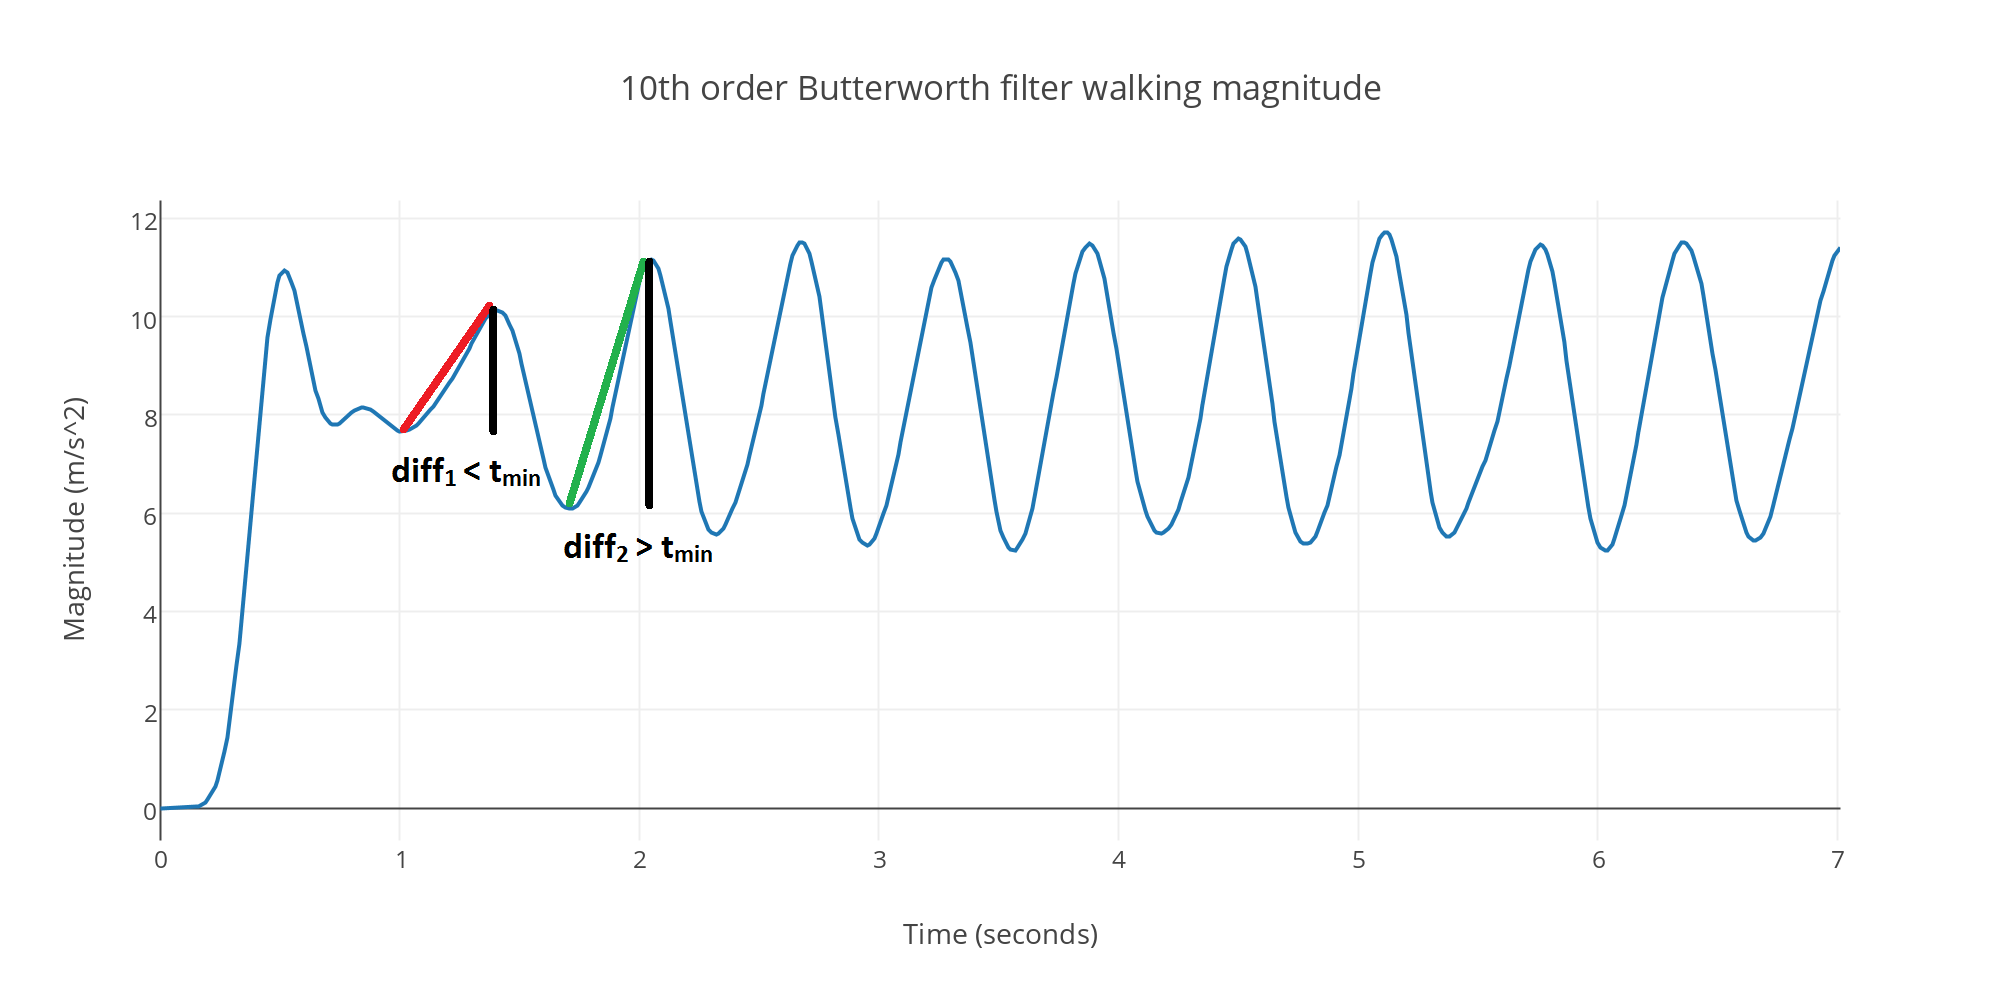
\includegraphics[scale=0.2]{images/butterworth10thOrderFilterWalkingMagnitudeThreshold.png}
\captionof{figure}{Applying minimum magnitude thresholding to avoid false positives}
\label{fig:butterworth10thOrderFilterWalkingMagnitudeThreshold}
\end{center}
In this case the magnitude difference between the second valley and second peak (not counting the first actual pair formed due to initial filter adjustment), represented by $\mathit{diff}_1$ in the graph, is below the minimum threshold $t_{min}$ and thus this pair does not trigger a step event. The magnitude difference $\mathit{diff}_2$ between the next valley and peak however is greater than $t_{min}$ and this counts as a step. For sudden hand motions, only the first 1-2 peaks will be produced in the filtered output and since both will ideally be below $t_{min}$ no false positives will be recorded. For standard walking, the first step will be recorded on the 3rd valley/peak combination in this instance. This approach also accounts for the previous `missed' pairs, which are actual legitimate steps in such cases, by keeping a record of valley/peak combinations that would have triggered a step but were below the threshold. Once the first step above $t_{min}$ has been detected the algorithm then knows that the previous peaks were not formed due to hand motions and counts those towards the step total as well. Note that a separate minimum threshold $t_{significant}$, which is smaller than $t_{min}$, is used to decide whether a valley/peak pair should be included in the record maintained. This ensures that very small peaks produced through slight sensor fluctuations rather than any actual motion are excluded.  

Initial tests with this approach showed that it was more robust with regards to false positives as compared to the first-order filter, with steps being recorded far less frequently for slight hand motions. However, with step detection during normal walking itself it was found that there was a noticeable lag between when steps were recorded and actually taken. This can once again be attributed to filter output computation being based on the large history of values, which results in any changes to the input being reflected a short while after they actually occur. As the first-order filter was deemed to be too sensitive and the tenth-order filter is too laggy, a fifth-order Butterworth filter, which uses 6 input and 5 filter output values, is used to attain the middle ground in the compromise between robustness and reactivity. The results of applying the fifth and tenth-order filters on the accelerometer readings for normal walking motion are compared in Figure~\ref{fig:butterworth5thVs10thOrderWalkingMagnitude}.  

\begin{center}
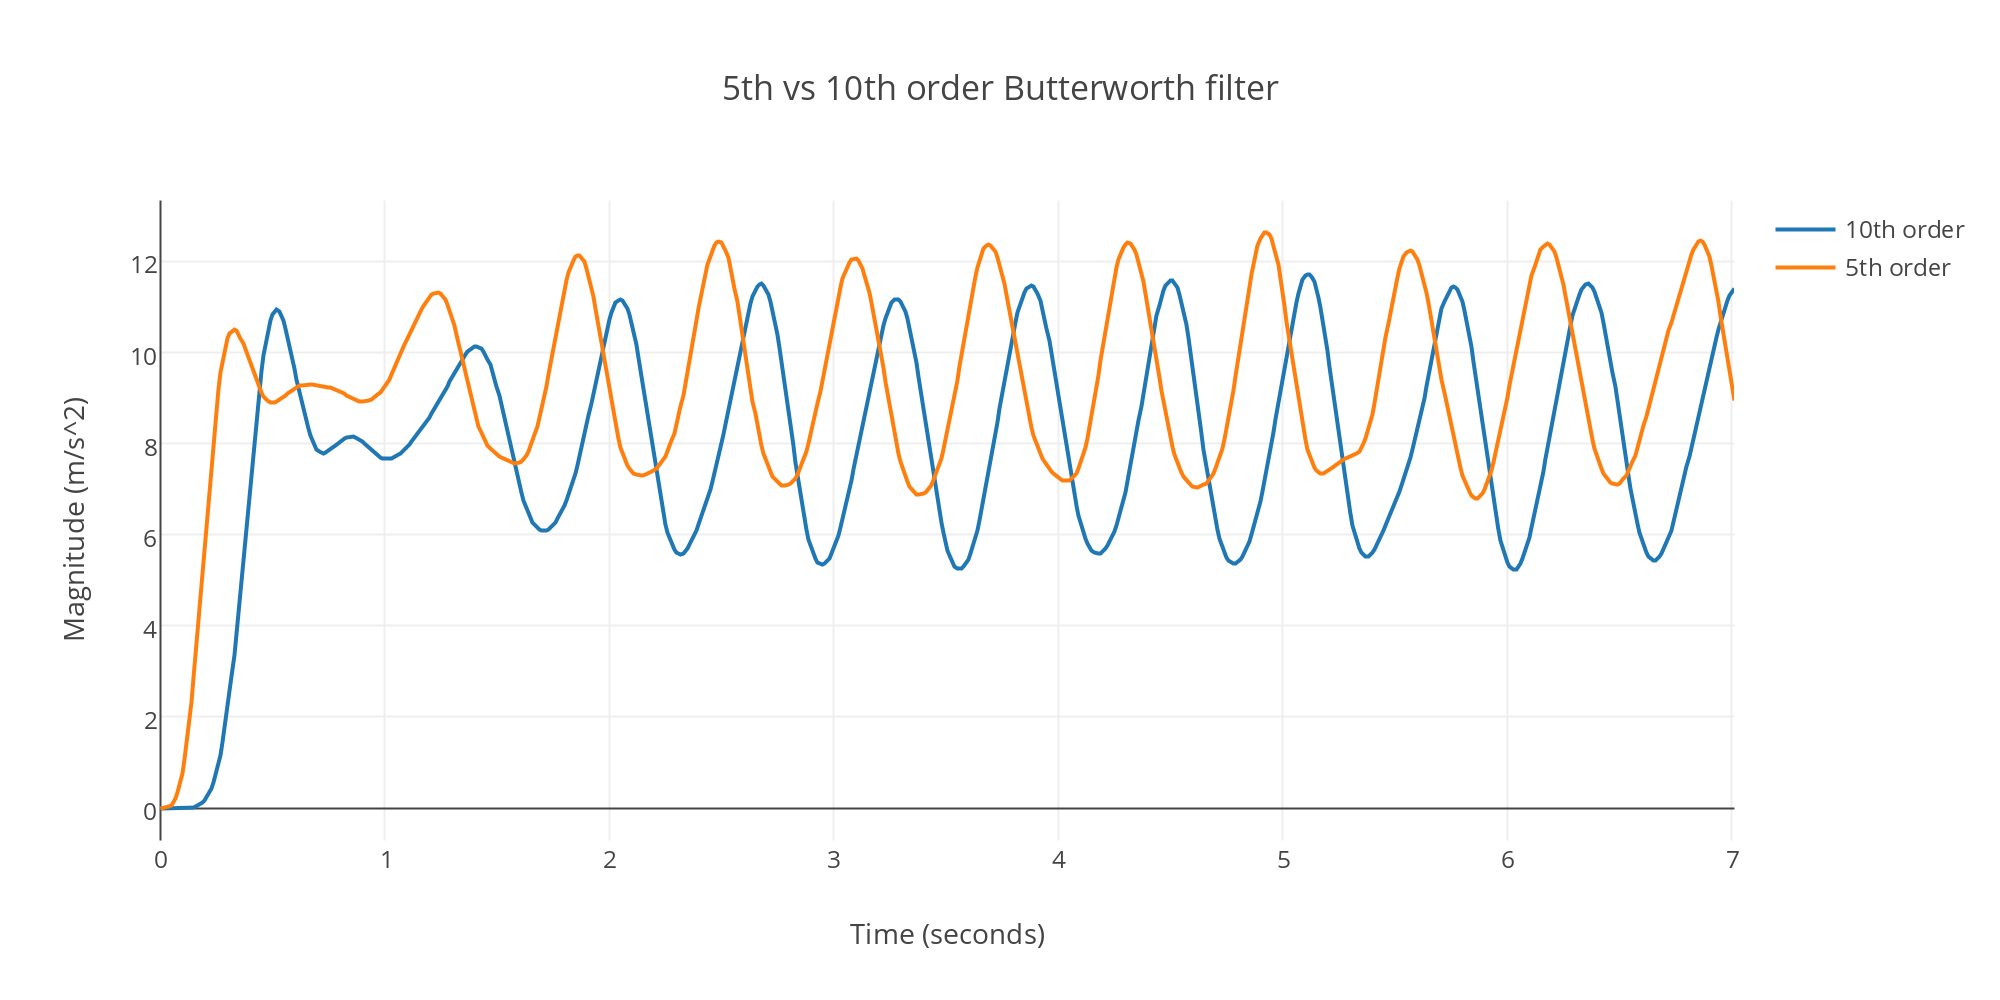
\includegraphics[scale=0.9]{images/butterworth5thVs10thOrderWalkingMagnitude.png}
\captionof{figure}{Comparing 5th and 10th order Butterworth Filters}
\label{fig:butterworth5thVs10thOrderWalkingMagnitude}
\end{center}

The shape of the 5th-order filter plot is almost identical to that of the 10th-order one, and all its peaks occur beforehand in tandem with when the steps are actually taken. Thus this 5th-order low-pass Butterworth filter is selected as the final one to use. 

\subsection{Vertical acceleration}

The magnitude of the 3-axis accelerometer readings was chosen as the measure for the step detection algorithm as it is a scalar quantity and thus independent of direction. This allowed step detection to be performed in the same manner regardless of the orientation of the phone. However, it is this directional independence that also poses a problem. The vertical acceleration of the user caused during their up and down movement while walking is the basis on which steps are identified; the horizontal acceleration does not provide any meaningful information in this regard. A scalar quantity like magnitude however is unable to differentiate between vertical and horizontal accelerations. Thus periodic movement of the phone in any direction, including purely sideways, can cause steps to be fired and contribute to false positives. The filtered accelerometer magnitude output when periodically moving the phone sideways from left to right is shown in Figure~\ref{fig:butterworth5thOrderFilterSidewaysMotionMagnitude}. 

\begin{center}
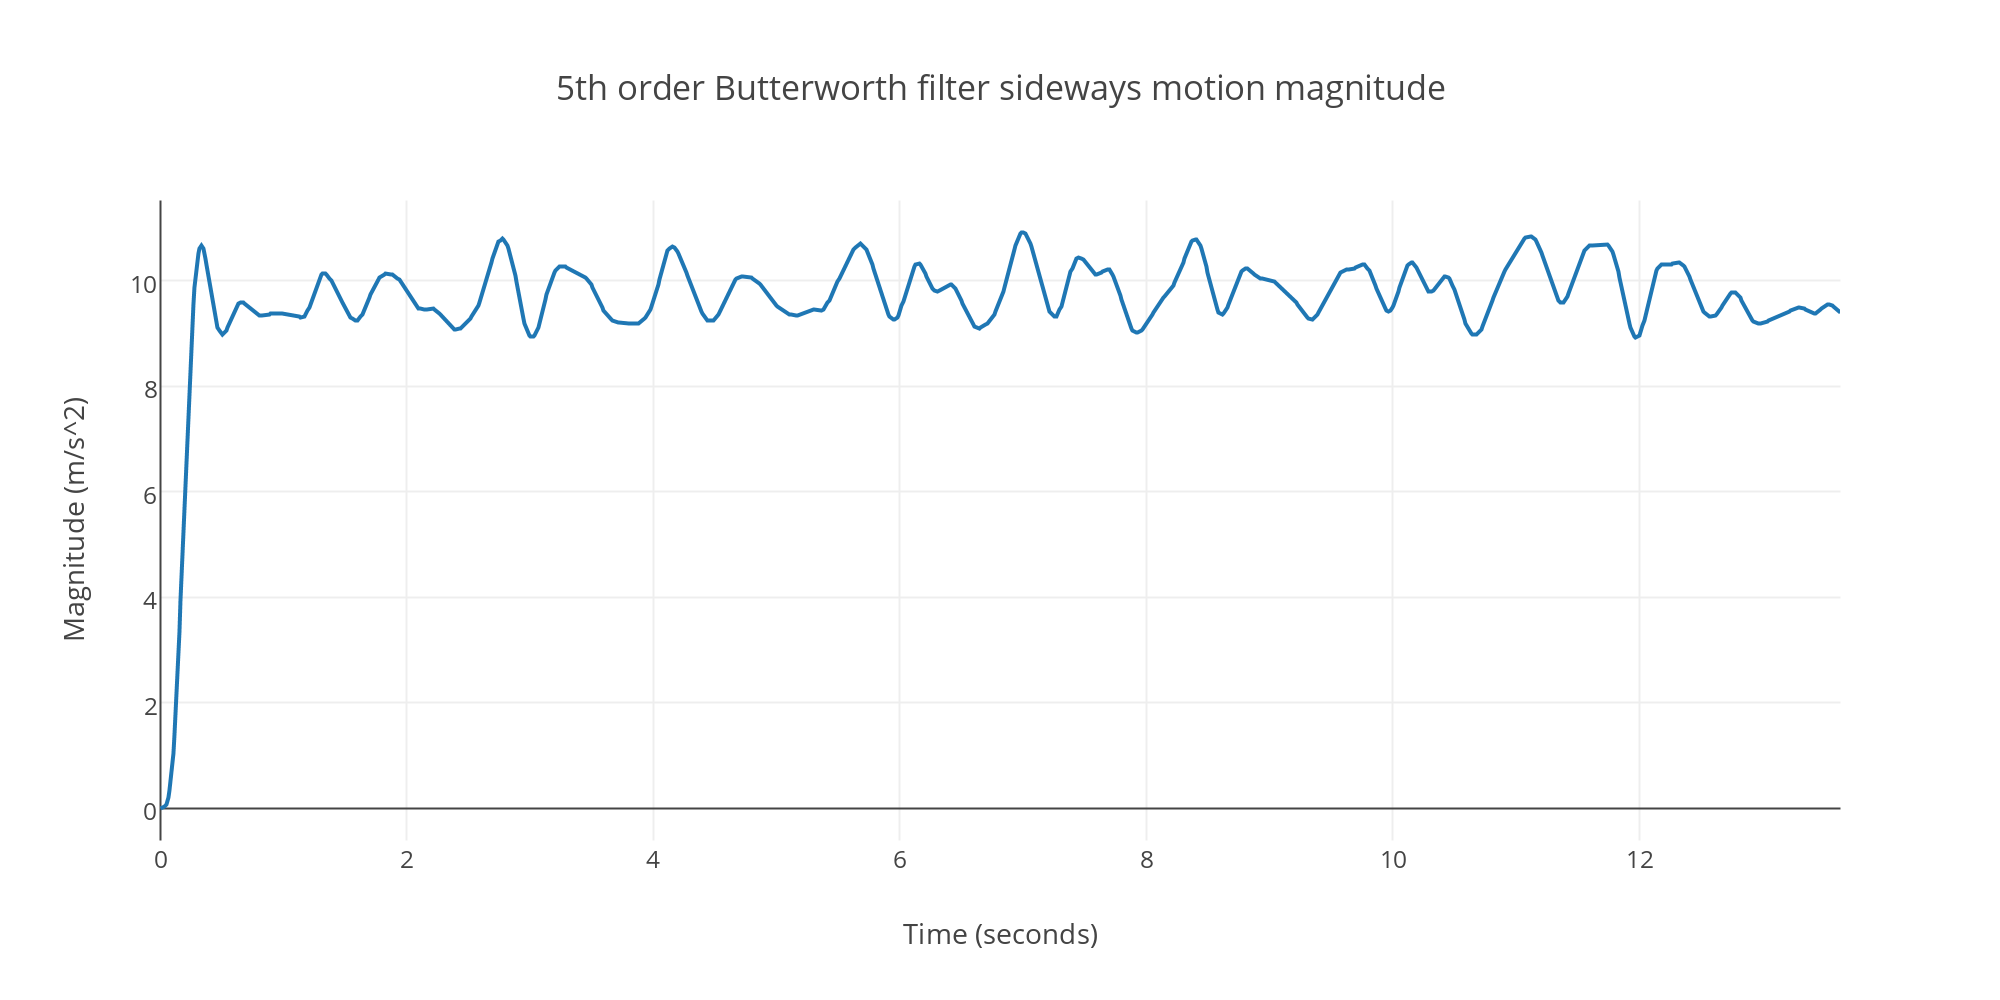
\includegraphics[scale=0.9]{images/butterworth5thOrderFilterSidewaysMotionMagnitude.png}
\captionof{figure}{Sideways motion magnitude}
\label{fig:butterworth5thOrderFilterSidewaysMotionMagnitude}
\end{center}
Thus it can be seen that it is difficult to determine on the basis of magnitude whether the variation in acceleration is due to the vertical component corresponding to walking motion or the horizontal component associated with other random motions. 

This problem is overcome by specifically tracking just the vertical component of the user's acceleration and using that as the measure for step detection. This is done by transforming the accelerometer readings from the device's local co-ordinate system to the world `East-North-Up (ENU)' co-ordinate system. The ENU system is depicted in Figure~\ref{fig:ENU}. 

\begin{center}
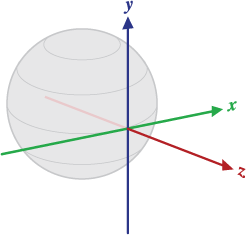
\includegraphics[scale=0.5]{images/ENU.png}
\captionof{figure}{The 3 axes in the ENU world co-ordinate system defined with respect to the Earth~\cite{ENU}}
\label{fig:ENU}
\end{center}
The Z-axis in the ENU system is defined to be pointing towards the sky and perpendicular to the surface, along the direction of the Earth's gravity vector. The Y-axis points towards the magnetic North Pole while the X-axis is defined to be the cross product of Y and Z, meaning that it roughly points East and is perpendicular to both the other axes~\cite{ENU}. From this definition it is evident that the vertical component of the user's acceleration in this system will be along the Z-axis, and thus exclusively using these readings would allow for any horizontal acceleration to be excluded from step detection. 

The mapping from the device to world ENU co-ordinates is achieved through use of a rotation matrix. This rotation matrix is obtained from a combination of the phone's gravity and magnetometer sensor readings, which provide the necessary orientation information to compute the matrix. The accelerometer readings in device co-ordinates are then multiplied by the inverse of this rotation matrix to convert them to the ENU system. Figure~\ref{fig:straightWalkVerticalAcceleration} provides an example of the filtered accelerometer readings for normal walking motion after mapping them to the ENU system. 

\begin{center}
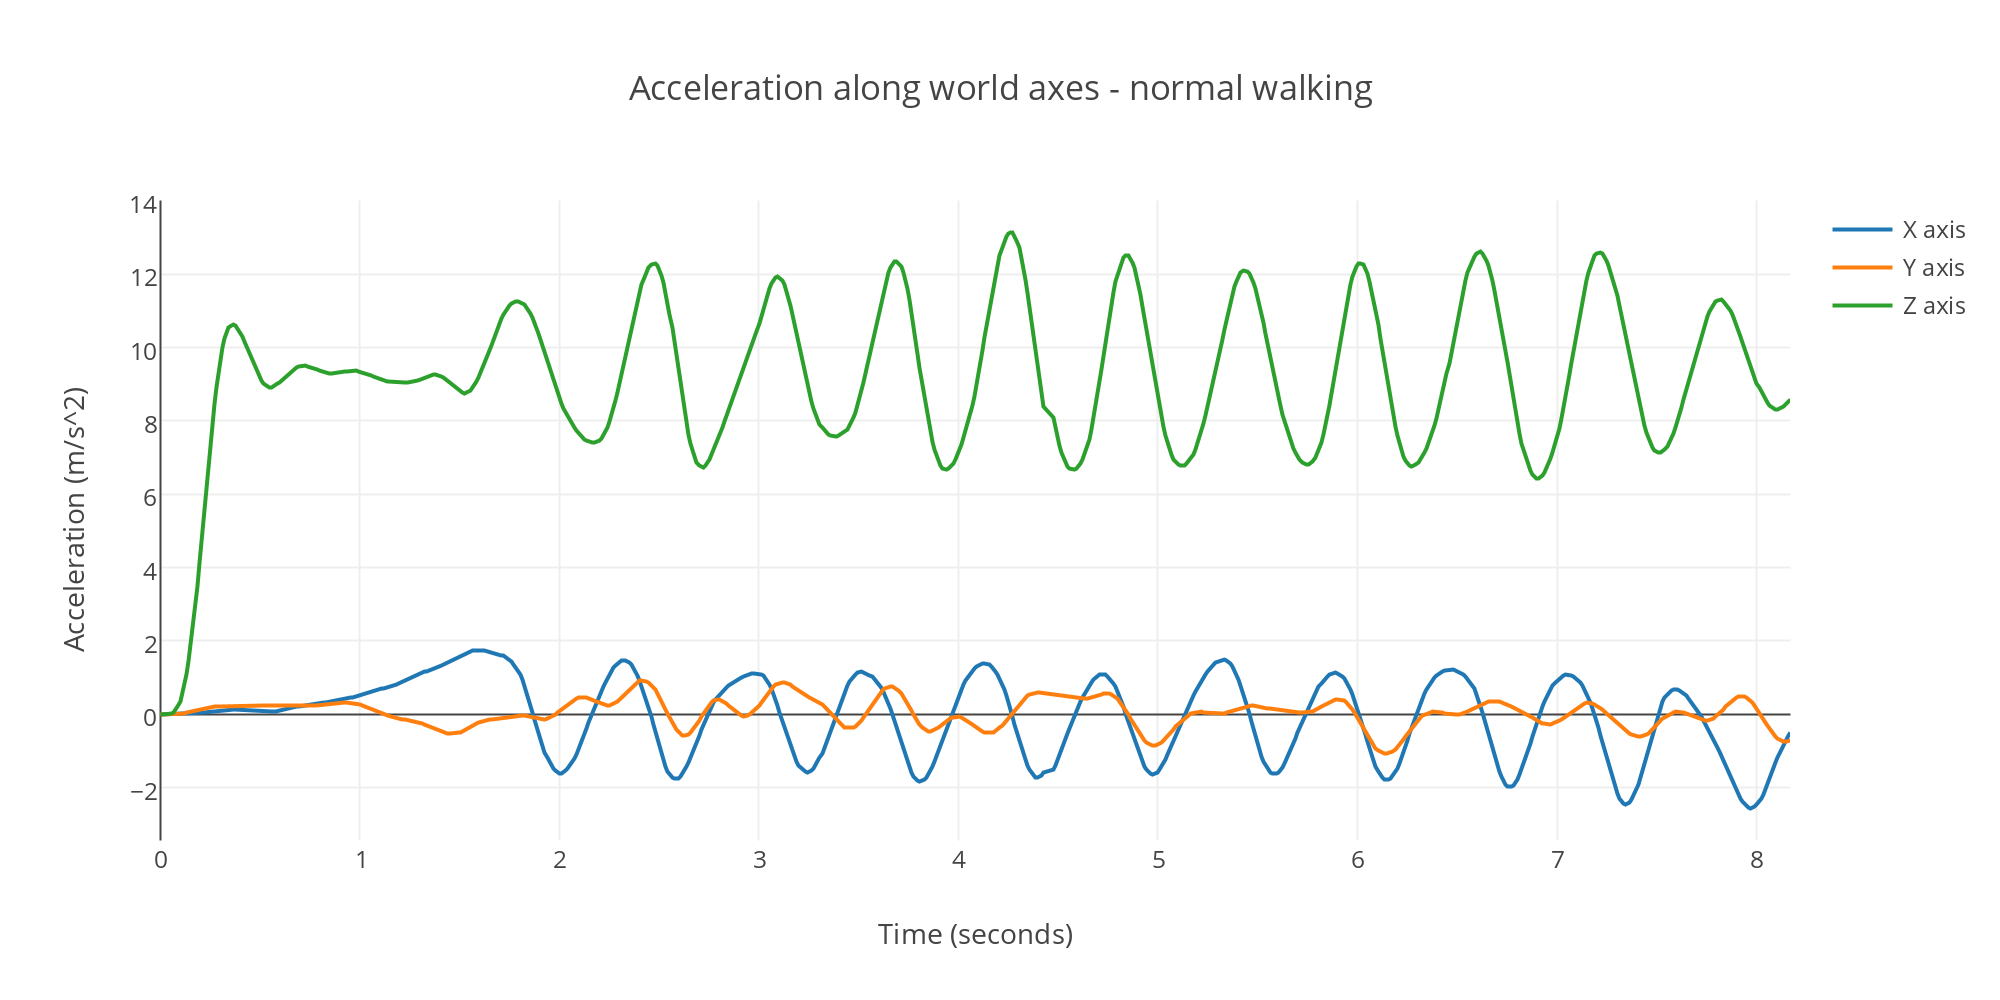
\includegraphics[scale=0.9]{images/straightWalkVerticalAcceleration.png}
\captionof{figure}{Accelerometer readings in ENU system for normal walking}
\label{fig:straightWalkVerticalAcceleration}
\end{center}
As seen in the plot, the Z-axis readings represent the user's vertical acceleration and thus fully defines the walking motion through peak/valley formation for the purpose of step detection. The Y-axis readings largely remain around 0 as the forward acceleration during walking is negligible, while the X-axis readings exhibit some variation due to the slight sidewards sway of the body while taking steps. Thus step detection can be carried out solely on the basis of the ENU Z-axis accelerometer readings.  

The robustness of this approach with respect to the magnitude readings is demonstrated by Figure~\ref{fig:sidewaysMotionVerticalAcceleration}, which depicts the filtered accelerometer output when moving the phone in a sideways manner.  

\begin{center}
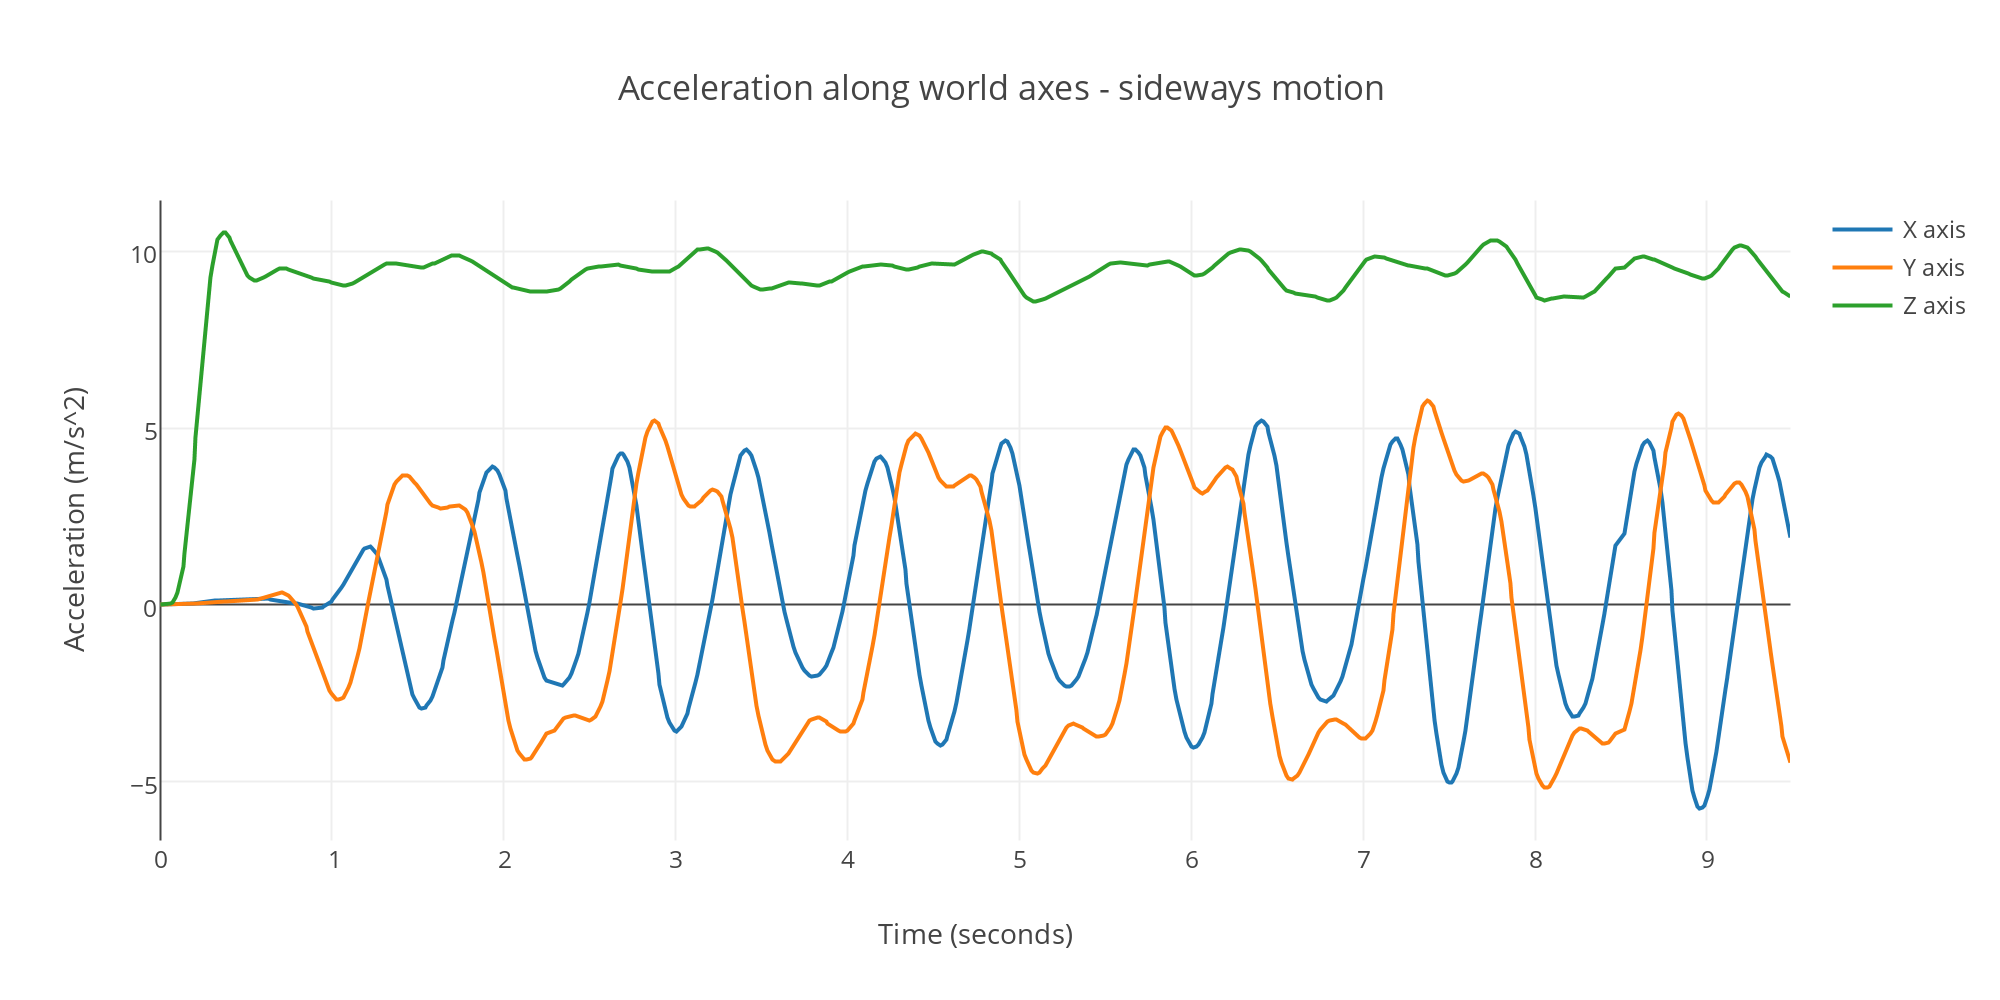
\includegraphics[scale=0.9]{images/sidewaysMotionVerticalAcceleration.png}
\captionof{figure}{Accelerometer readings in ENU system for sideways motion}
\label{fig:sidewaysMotionVerticalAcceleration}
\end{center}
In this case the variations are along the X and Y axes. The Z-axis readings however remain largely flat since sideways motion does not produce vertical acceleration. Thus it is far more unlikely for such movements to result in false positives in the ENU system as compared to using the magnitude of the acceleration for step detection. 

\subsection{Further Optimisations}

Using the Butterworth filter and accelerometer readings in the ENU system results in step detection that is accurate and responsive while also being fairly robust to false positives. However there are still occasional cases where unrelated movements cause steps be recorded. Thus the following additional constraints derived from characteristics of typical human gait are applied to further reduce the likelihood of false positives occurring.  

\subsubsection{Thresholding}

A minimum threshold $t_{min}$ for the absolute difference between adjacent valley/peak accelerations was discussed in the previous section for differentiating between momentary hand motions and normal walking motion. This minimum threshold also ensures that very slight fluctuations in acceleration value due to noise or any other external factors do not trigger a step. This idea can be extended by noticing the fact that the accelerations produced by standard walking usually lie within a certain fixed interval. Any acceleration considerably larger than the maximum value of this interval is likely to have been generated from a motion other than walking. Thus a maximum threshold $t_{max}$ is also applied to the accelerometer readings. The difference between an adjacent valley and peak must be above $t_{min}$ and below $t_{max}$ for it to be recorded as a step. 

\subsubsection{Peak to valley difference}

Steps are currently detected solely on the basis of the acceleration difference from a valley to its corresponding peak. The absolute acceleration in the downward phase of a step is expected to be roughly similar to that in the upward phase for standard walking. Thus the condition that the peak to valley difference must be within a certain percentage of the preceding valley to peak difference for it to be classified as a step is introduced. This means that any step is now actually recorded at the valley following the peak.   

\subsubsection{Time difference}

It was noted in the previous section that the frequency of normal walking motion ranges between 0.7-3 Hz. Assuming 3 steps to be the maximum taken per second during walking means that the time interval between subsequent steps is at least approximately 330ms. Any smaller time difference suggests that the recorded motion is too quick for it to be standard walking. Thus allowing for a small margin, a minimum requirement of 300ms between consecutive steps is set in the application. If a valley is found to occur before 300ms have passed since the previous one, the step associated with it is ignored and not added to the overall count.

\section{Path Finding Algorithm}

\subsection{Practical motivation}
While the main aim of the application developed by this project was to actively track user movement within a building, we realized that making use of path finding will greatly benefit the project as well. This resulted from information obtained from other sources, where certain positions in buildings were utilized in order to reset the error caused by the sensors. On top of that, this addition resulted in an easier to understand interface as well as aiding the user in the search for their destination. In order to add a path finding algorithm to our project, we decided to investigate the different available options and evaluate their performance in order to identify the optimal algorithm.

\subsection{Path finding algorithms considered}
The previous sections detailed how we extracted a graph structure from the image data provided for each floor. This graph structure can be thought of as a mesh, representing walkable areas of the floor via vertices and edges. There are several algorithms that are capable of performing path finding on this type of data-structure and we selected the most popular ones for our testing. 

\subsubsection{Dijkstra}
This is a shortest path graph path finding algorithm. While there are many iterations, the two major versions differ greatly. Initially, this algorithm searched for the path only between the two specified nodes (start and end node), however the later versions, being the more prevalent ones nowadays, perform this kind of calculation on all nodes in the graph. This means that if we specify a node within the graph as our finish node, the algorithm will calculate the shortest path from all of the other nodes in the graph to this node. While this seems inefficient, the reason for this is the minimal performance hit incurred by performing this operation, as well as the possibility of these results being reused at a later run of the algorithm. These kinds of implementations therefore make heavy use of caching. The base runtime of Dijkstra's algorithm is $O(V^2)$, where V is equal to the number of vertices in the graph. This can however be further optimised by using the altered implementation of the algorithm by Fredman \& Tarjan\cite{algoImprovedDijkstra}, where the implementation is based on a min-priority queue that makes use of a Fibonacci heap. This kind of implementation runs in $O( E + V + log(V) )$ , where E stands for the number of edges in the graph and V stands for the number of nodes. Thanks to this change in implementation, Dijkstra is one of the fastest shortest path algorithms that can be used for arbitrary directed graphs with a single restriction that dictates that edge weights have to be non-negative.


\subsubsection{A*}
A* is an informed graph search algorithm that makes use of heuristics.  An informed algorithm functions on the premise of solving a problem by searching for the solution amongst all of the solutions available for a given graph. While this might seem inefficient as there can be millions of ways to traverse a graph, A* employs two measures to greatly reduce the subset of solutions. It does this by utilizing two measures for each node:
\begin{itemize}
\item g(n) - This function represents the cost of the path required to reach a specific node n. A cost in this case can be anything ranging from distance to petrol required to travel. Using this function ensures that any specific solution is aware of the requirements to get into the state it is in.
\item h(n) - Represents the estimated cost of travelling from a specific node n to the target finish node. We can use multiple estimation techniques depending on the knowledge of environment, such as Manhattan distance or Euclidean distance.
\end{itemize}

The strength of A* comes from combining the two measures explained above into a single measure, allowing the algorithm to estimate the best partial move when traversing a graph. This makes A* a very flexible and strong candidate for path finding on graphs. Therefore, it is also highly favoured in games.

\subsubsection{Recast}
The last algorithm considered was the Recast\cite{libRecast} algorithm, now commonly used in games. It originates from a game navigation construction toolkit. The Recast approach makes use of heavy pre-processing of the input meshes. The only restriction for the input mesh is for it to consist of triangles, this is then pre-processed into voxel mold, which then in turn allows the algorithm to estimate walkable spaces and perform a conversion to convex polygons. Once the conversion is complete, Recast is then able to make use of the polygons to reason about walkable space, taking into account measures of an agent (such as height or width).
\newline

Recast offers a great deal of flexibility and has an excellent turnaround time. The fact that it allows for real-time modification of the mesh and is able to respond to changes in it further allows for possible extensions of the project such as obstacle detection (moved furniture for example) or others. While this does require additional levels of pre-processing, the potential performance gain is significant enough to benchmark this algorithm.

\section{Wall Collision Algorithm}

The purpose of this component is two-fold. Firstly, to give the dead-reckoning system a sense of walls and the limits they enforce on movement. Secondly, to ensure that any error from not taking into account walls is not introduced. The basic concept is that when the application believes the user has taken a step in a given direction, it verifies that step can logically be taken. For example if a step is detected and user is facing a wall, the system should not believe that the user has moved through a wall.

\subsection{Initial Implementation}

For the initial implementation, the extracted floor plan graphs are used as the basis for deciding whether a step the systems believes the user has made is valid or not. These graphs have one important feature that allows for this, two adjacent nodes are not connected if there is a wall between the corresponding positions in the floor plans. This allows for the following procedure to determine if a step is valid:

\begin{itemize}
	\item \textbf{Assign the nearest node to the user} - The node nearest to the user's estimated real position is assigned to the user, this can be used for path finding a new route if required, or in this case determining the validity of a movement. The nearest node was originally found through a brute force search, though this was later changed to a more efficient modular arithmetic method that exploits the known distances between nodes to center on the nearest node in O(1) time.
	\item \textbf{Simulate a step} - A step is then simulated from the user's real position, this is essentially calculating where the user will move to given their current heading and rough stride length estimate. The stride length was initially set to the equivalent of 12 pixels in the floor plans, since the distance between nodes is 10, therefore allowing for proper testing. 
	\item \textbf{Check for new nearest node} - From the new simulated real position, check if there is a new nearest node:
	\begin{itemize}
		\item If there is a new nearest node, path find from the first nearest node to the new one. If path length is greater than 2 the user must have transitioned over a wall, see Figure~\ref{fig:iniCol} for an example. If the length of the path is less than or equal to 2, the move is valid
		\item If the nearest node does not change then the move is valid
	\end{itemize}
\end{itemize}

\begin{center}
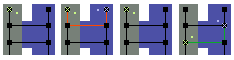
\includegraphics[scale=1.5]{images-implementation/collision1.png}
\captionof{figure}{Diagrams showing the above steps, the lefthand pair is a step being rejected due to a path length of 3, the righthand pair accepts the step as valid}
\label{fig:iniCol}
\end{center}

\subsection{Issues}

This implementation serves its purpose but it was ultimately scrapped due to the following two reasons:

\begin{enumerate}
	\item The initial implementation is gated by the distance between two nodes. If the stride length is greater than two and a half times the number of pixels between nodes, then every step will have a path length greater than 3. Meaning every step is then rejected, the step length we found to be the average of our groups equated to around 30 pixels. This problem can be bypassed by simply running the method over 30 pixels in 3 chunks of 10.
	\item Due to the reliance on path finding, it heavily slows down the application to unusable levels. This is exacerbated by the need to repeat it multiple times to work over the set stride length
\end{enumerate}

Whilst the first problem was fixable, the second was not without creating a new method, the implementation below was made to solve this issue.

\subsection{Final Implementation}

With the initial method being too slow, another one was developed. Instead of working directly with the graph, which causes the slow down due to path finding, it works with the raw hand curated floor plan image. It directly looks at the colours of pixels within this image to determine if the path from start to end would have crossed a wall, a white pixel.

It does this by taking the co-ordinates of the current nearest node and the new nearest node from the simulated step and creating a path, pixel by pixel, between the two node locations. It decides whether to move in the X and Y direction by examining which of the difference in X or Y between the path's head and end point is larger. It selects the larger difference and then assesses which direction it needs to move by checking which co-ordinate of the two locations is larger. For example, to move left the difference between the path's X and end's X needs to be greater than the Y difference of these two points and then the path's X is greater than the end's X co-ordinate.

Once the next pixel in the path has been chosen, the method then checks the colour of that pixel. If it is white then the user's step will hit a wall and it classifies the step as invalid. If the pixel is not white the method continues pathing between the nodes. This repeats pixel by pixel until the end location is reached and now the move is considered valid as no white pixels existed on the path.

This proved to be a much faster method and removed the lag that was being experienced with the previous method, since the cost of loading the image (which occurs when the application is first opened) and the cost of checking pixel colours are both less than the cost of running the path finding algorithm.

\chapter{Implementation}

\section{Smartphones}

As can be seen by figure ~\ref{fig:phoneMarketShares}, the smartphone market is heavily dominated by devices operating the Android operating system. iOS devices produced by Apple come in second, and together both Android and iOS devices comprise about 95\% of the world smartphone market. With this in mind, we analysed the hardware makeup of the smartphones that run both operating systems. \\

\begin{center}
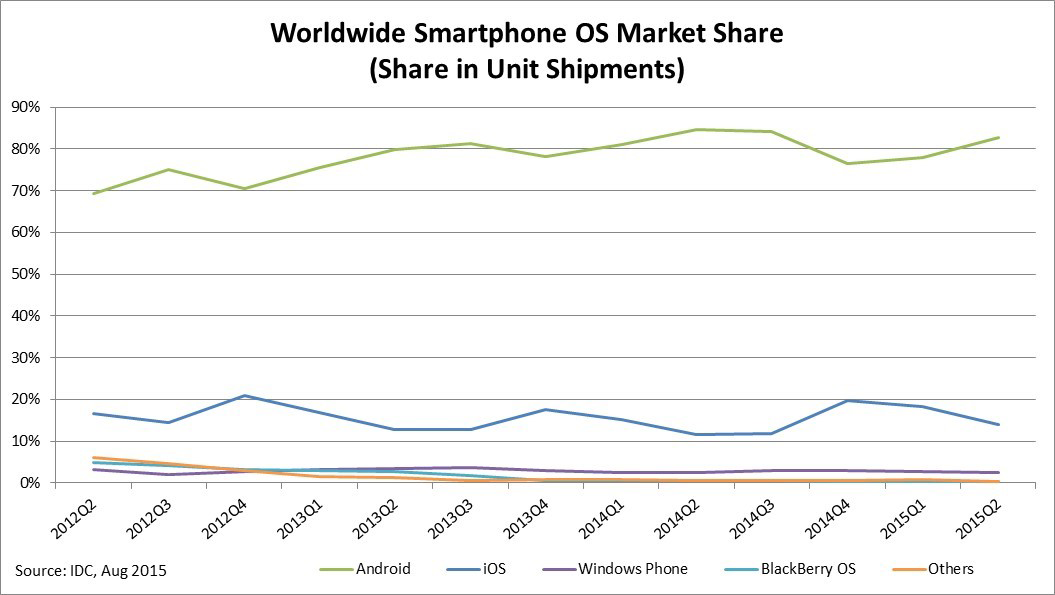
\includegraphics[scale=0.7]{images/phoneMarketShare.png}
\captionof{figure}{Smartphone operating system market shares ~\cite{phoneMarketShare}.}
\label{fig:phoneMarketShares}
\end{center}

Amongst the team, there was an even 50/50 split between owners of Android devices and owners of iOS devices. Considering the fact that development would occur around our own personal devices, we decided to highlight the most advanced device from each operating system that we had access to as the target of our research. These were the iPhone 6 and Motorola Moto G (2nd Generation).

\subsection{iPhone 6 Hardware}

The iPhone 6 contains all of the sensors one would need for the production of an indoor navigation system that relies primarily on inertial sensors. The iPhone 6 comes equipped with an accelerometer, three-axis gyroscope, barometer and digital compass, amongst other sensors ~\cite{iosSpecs}. These relay data to the iPhone's built in M8 coprocessor chip, which is designed to offload the collection of sensor data from the central processing unit (CPU). The M8 coprocessor collects, processes and stores the sensor data when the phone is powered down, allowing this to be accessed upon powering up, helping to conserve battery life ~\cite{m8}. The coprocessor is able to be accessed using the Apple provided Core Motion API. We would make extensive use of this API in order to produce our indoor navigation application. The screen offerings are large, with the iPhone 6's 4.7 inch and iPhone 6 Plus's 5.5 inch screen both offering a sufficient screen area within which to display the application.

\subsection{Motorola Moto G (2nd Gen) Hardware}

The Motorola Moto G also contains an accelerometer, gyroscope and compass, but lacks the barometer offered by the iPhone ~\cite{motoSpecs}. This phone also does not contain a dedicated coprocessor that handles sensor data. A major distinction between Android and iOS operating systems is that the iOS systems and the devices that operate them are developed concurrently. This means that both the hardware and software are optimised for each other, allowing for specialised features such as the M8 processor to be produced. Android must contend with a wide variety of hardware platforms and specifications, meaning its features are typically more limited. The 5 inch screen however offers a large area within which to display the floor plans and user interface of the application.

\subsection{Choice of platform}

As can be seen, the sensors offered in both smartphones mean that an indoor navigation application is theoretically possible on both platforms. This coupled with the fact that our project team each only had access to either one operating system or the other, not both concurrently nor all the same platform, we decided that the best course of action would to be pursue a joint iOS and Android application. This would also reflect the real world distribution of hardware amongst people, allowing a final application to be used by the largest cross section of users possible. This naturally led us to investigate how this could be best achieved.

\section{Development Platforms}

Both Android and iOS devices have their own development kits that run on their own unique programming languages.

\subsection{iOS Development Platform}

Development for iOS is limited to Apple produced computers (MacBooks, Macs etc.). The integrated development platform (IDE) offered by Apple is Xcode ~\cite{xcode}. At the time of writing, Xcode is offered free on the Mac application store for users of the `El Capitan' Mac operating system. iOS development can occur in both the Objective-C and Swift programming languages. Both are object oriented languages, with Swift being a newly created language by Apple, introduced at Apple's 2014 Worldwide Developer Conference (WWDC), offering several benefits over the older Objective-C, amongst these added brevity and a greater resilience to erroneous code ~\cite{swift}. No team members were familiar with either of these programming languages, with only one member having used Xcode previously, but for a project written in C++. A further restriction existed in the fact that only half the group team members owned any kind of Apple computer, meaning they would be unable to develop anything within Xcode.

\subsection{Android Development Platform}

Android also provides its own IDE called Android studio ~\cite{androidStudio}. This is available across all computer operating systems (Windows, Mac and Linux) and can be downloaded from their website. Applications for Android are written in Java, with the IDE also providing a wide range of supplementary profiling and debugging software. All team members were familiar with Java, with it having been a major part of the Computer Science course to date.

\subsection{Shared Development Environment}

Xamarin is a company owned by Microsoft that develops the Xamarin Studio IDE ~\cite{xamarin}. Xamarin offers the ability to code applications for Android, iOS and Windows Phone with a C\# shared codebase, with all of the latest iOS and Android API libraries ported over into C\# and code able to be shared across the various platforms. Xamarin.Forms, introduced in 2014, goes as far as to allow implementations of shared user interfaces.

With their website citing the ability to share up to 90\% of code across applications on multiple platforms, we were attracted by the prospect of being able to have a singular application work on both iOS and Android. Furthermore, two team members were already proficient in C\#, with one also having worked previously with Xamarin.

\section{Floor Plans}
    
Floor plans played a major role in the design of the application. Not only would the Computer Science building's floor plans be used to produce the graph that would be used for pathfinding and navigation, it would also provide the backdrop upon which the majority of the application would be displayed. With this in mind, floor plans went through a protracted phase of pre processing and refinement, allowing us to retrieve the information we needed and visually enhance the images as well.

\subsection{Selection of the Images}

Although we initially considered creating our own floor plans from scratch by physically measuring room dimensions and producing images from these figures, we found out that floor plans suited for our needs could be obtained from the University's online interactive map. The interactive map contained floor plans of all the University's academic buildings, made publicly available through their website. Retrieving the images from this website was beneficial for various reasons.

\begin{itemize}

\item They are created to-scale, allowing us to rely on the proportions of the floor plan. This was crucial for our needs as we needed to represent real world movement with the movement of a cursor on the image. Any discrepancies between the scaling of the image and the real world dimensions of the Computer Science building would add unwanted error to the system.

\item The images contained additional information that benefited our application as well. This comprised of room numbers, symbols for utility rooms and so on.

\item Floor plans for different buildings could be obtained with ease, allowing us to possibly expand the application to other buildings if needed. This was a consideration for further testing should we run into issues with testing within the Computer Science building.

\item They provided us with a good conceptual outline that could be utilized at later stages of our project, where we would ultimately design our own floor plans to suit the appearance of the application.
\end{itemize}
		
\subsection{Image Processing}

Despite the benefits, several issues still existed with the provided floor plans. The images available were often too complex for any immediate processing to take place and contained a lot of noise in the form of labels or icons. This kind of superfluous data, whilst visually appealing, is obviously not suitable for the extraction of a graph, for example, from the floor plan (based on our plans to make use of a colour based algorithm) and therefore it was decided that, in order to make use of the available resources, hand curation was necessary.

The process of hand-curating the images involved the following steps:

\begin{itemize}

\item Limiting a room to a single colour - This was a requirement as some rooms made use of gradient colours. Keeping these could greatly hinder the extraction process and the gradients were therefore removed.

\item Removal of labels and other text - The room numbers and other information would be stored within a separate file and therefore were unnecessary when working on the graph extraction.
			
\item Normalizing the colours of walls - Some of the walls and space outside the building were not completely white as they were dissolved by the gradients. Making all of the walls exclusively white was crucial for the success of the graph extraction process.
			
\item Widen the doors in order to compensate for build-up error of sensors - This was necessary at the later stages of the project, where we realized that the build-up error of the sensors could stop us from navigating through doors.
\end{itemize}
		
\subsubsection{Benefits}

Having a hand curated image allowed us to perform easier extraction of the navigation graph and also introduced other possibilities on handling the further challenges in the implementation. The hand curated image is further used in wall-detection as well as other support systems for navigation. 
		
\subsection{Graph extraction}

The hand curated images were then able to be used for the extraction of the graphs.

\subsubsection{Considerations}

When extracting the graph from the hand-curated images, the project encountered many issues related to the difference in performance of mobile devices as well as restrictions when processing specific device OS. It was therefore decided to pre-extract all graphs from the images and only use the post processed files in order to remove the on-device processing dependency. While this has downsides as well, the performance cost is significantly smaller.
\newline
		
Another significant point when considering extracting the graph was the storage method on the device. Unlike PCs, phones and similar mobile devices utilize significantly smaller overall storage space and therefore we could not accommodate for large, dense, and fine graphs. We were therefore obliged to find a balance between increased separation between nodes in the graphs in order to reduce graph file size and also ensure that the distances between nodes were small enough to allow for accurate movement and path creation.
\newline
	
The last significant part of our considerations for this process was the representation of additional data present in the picture. We required a way of navigating a user from specific rooms as well as allowing for functionality such as filtering of rooms per floor. At the same time we had to balance the benefit gained from keeping data readily available in memory, and the limits on memory used by an application imposed by Android and iOS.

\subsubsection{Initial approach}

As per the decision explained in the previous section, all of the graph extraction was performed using a computer instead of real-time extraction on the device. This has allowed us to make heavy use of parallelism as well as methods exploiting non-PCL libraries.
\newline
	
Our initial version of the extraction algorithm utilized the hand curated graph we created by using a version of flood algorithm. This was performed by setting an initial point in the middle of the picture (or in any room)  and creating nodes and edges by flooding in 4 directions. This was bounded by simple logic, where no nodes were created in walls (white colour). While this approach worked, it had many performance issues due to objects in the .NET API - namely Bitmap. The GetPixel method was not thread safe and therefore was locking the Bitmap data before accessing it. It was therefore obvious that the subsequent iterations that will require more than a single iteration over all of the elements will have to overcome this problem

\subsubsection{Optimisation}
While the initial tool was capable of extracting a graph from the image, it caused many issues in regards to runtime and the overall size of the graph produced. In order to mend these problems we decided to re-implement the tool with the issues from the previous version in mind. 

\subsubsection{Removing the bitmap object dependency}

The only way of exposing the pixel data in the Bitmap object was to use its GetPixel method. This method is not thread safe and was therefore locking. This caused issues when an attempt at using parallelism with the project was made. In order to remedy this, raw data of the bitmap image was stored in a two dimensional array, expressing information about the image. Thanks to this we were not only able to access the pixel information from multiple threads at once, but also ensure that the access time for an individual pixel is O(1), thanks to direct indexing. 

\subsubsection{Node distance}
In the vanilla version, each pixel represented a node in the graph. After running tests and comparing the measures, it became apparent that this approach is not feasible due to three separate reasons:
	
\begin{itemize}

\item Produced graph was too large - the graph created using this method contained up to 2.5 million nodes. This resulted in overall graph sizes of over 150 MB, which is extremely large for a mobile application.

\item Loading the graph on the device took a long time due to the need to deserialize nodes and edges.

\item The graph pathfinding library used was struggling with the large amount of nodes and vertices, delaying the response time from a few hundred milliseconds to a few seconds. This was not suitable for real-time navigation.

\end{itemize}
	

\subsubsection{Two-directional linking}
	
The initial version was forcing each node to check all four directions for possible neighbours. This was redundant as the same effect could be achieved by checking only two directions in an undirected graph. The solution was therefore adapted to only check left and right from each node created in search for neighbours.

\subsubsection{Introduction of multi-pass graph generation}
The initial version also suffered from severe inter-loop dependency. This was caused by the fact that in order to create an edge, all of the vertices had to be already created - otherwise we could miss some of them. This caused the separate threads to block each other. In order to resolve this, multi-pass was adapted.  The optimised version therefore processes separate stages sequentially, while each individual stage exploits parallelism.

\subsubsection{Runtime summary}
The optimisations greatly improved the runtime of the extraction. Thanks to the usage of direct indexing and hashing, we were able to ensure that the extraction process didn't take longer than a few seconds to perform all the steps necessary in order to generate a graph. The initial generation of nodes for the graph runs in the time O(n) as it needs to check each position on the image for a possible node. Each operation with pixels runs in O(1) thanks to the ability to directly index into the pre-processed array. The linking operation runs in a combined time of O(n * log(n)) + O(2n) due to the need to check two directions for possible links as well as locating a node in a collection. The collection of nodes is represented by a Dictionary type, which loosely translates to a HashMap. 

\subsubsection{Saving and loading}
The project utilizes XML as its means of storage. This is due to multiple reasons:
	
\begin{itemize}

\item The robust nature of XML based storage is a good match for this project as its ensures validity checking as well as allowing for easier understanding of the data present. Using this approach also opened up the graph data structure to modifications beyond the scope of edge and vertex data. 
		
\item The language we chose - C\# - has great support for XML data. It allowed us to utilize serialisation and deserialization of objects into XML, resulting in easier integration and faster loading times.
\end{itemize}

\subsubsection{Benefits \& Limitations}
By implementing our own custom extraction as well as loading and saving methods for the graph, we have managed to work around the restrictions imposed by the existing methods and utilize the full potential of having access to floor plan data. Our decision to keep room data and navigation data in separate files further enabled us to allow the application to handle arbitrary amount of floors, by simply having a reference handle to files that involve navigation without loading the floor plan into memory. The finalized data storage method is flexible and therefore can be updated at later stages without the need to re-generate all floors for a given building.
\newline

The extraction method was heavily optimised for speed using only a few steps to reach the final graph as shown in \textbf{Figure[\ref{fig:nav_graph}]}. This approach was adapted to ensure we can extract floor plans from different buildings for later tests, if need be. This has encouraged us to make heavy use of parallelism in our extraction process as well as a series of methods that allow us to access image data directly. 
\newline

By utilizing the methods explained above, we were aiming to decrease the amount of processing required to be performed on the device and this should therefore benefit user experience. We encountered several issues with mobile devices, where in both cases iOS and Android we reached the maximum memory allowed per-application and therefore had to re-design our approach to loading floor plans multiple repeatedly, eventually arriving at an optimal solution.
\begin{figure}[h]
\center
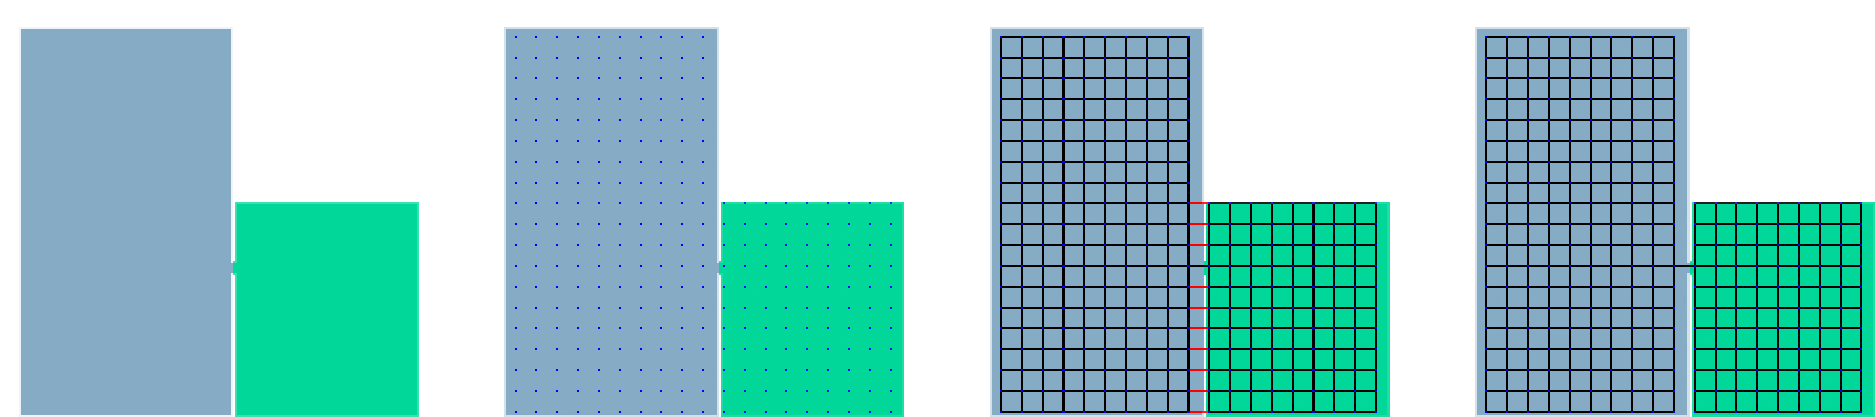
\includegraphics[trim=0 0 0 0, clip,width=\textwidth,height=\textheight,keepaspectratio]{images/graphGeneration.pdf}
\caption{Steps in generation of the pathfinding graph, from the initial hand curated image to full navigational graph.}
\label{fig:nav_graph}
\end{figure}

\section{Pathfinding Algorithm}

\subsection{Existing libraries}
Due to the fact we decided to develop in C\# and make use of Xamarin studio, we were able to locate PCL compliant libraries able to be deployed on our mobile devices. These libraries make use of our previously pre-processed graph data structure that can be interpreted as a mesh. This allowed us to easily adapt our extracted data to the needs of each library we investigated. Each library we tested offered a different implementation of one (or multiple) of the algorithms mentioned above. As discussed before, some implementations make use of caching in order to speed up their subsequent operation, while others focus on refining the data structures that are responsible storing the graph representation. This allowed us to observe the impact of the two solutions on the mobile device.

\subsubsection{SharpNav}
This library\cite{libSharpnav} is a PCL compliant non-native port of Recast. The version we used was labelled "SharpNav.Mono" which was able to be run on our Android devices. Our tests conducted using this library have shown promise, however due to the early stage of development of this library, its PCL variant offers very little support when it comes to loading pre-processed data. This would mean we have to do all three stages of pre-processing on the device, which was not acceptable due to the long time required to do so. This also required all three of the data structures (mesh, voxel mold and convex polygon representation) to be stored in the device memory, resulting in the host application encountering memory related issues. We were therefore forced to move away from using this library, as it was not a good match for a limited space a mobile app has allocated.

\subsubsection{Urho3D}
The second option we considered was the Urho3D game engine, which is partially developed by programmers at Xamarin. This engine\cite{libUrho} is capable of creating, saving, and performing operations on a mesh pre-processed by Recast. In order to utilize these elements of the engine, we were required to create test applications containing other base elements first. Therefore, we quickly realized that, in order to access the path finding of this library, we were required to create three additional objects. Namely this was Scene, which hosted all of the "game objects", followed by a Mesh object representing a collection of all the mesh within the scene and, finally, our particular piece of mesh. Doing this also added additional payload to our application, as the engine was packaged with it, increasing the size of our application by nearly 6MB. Upon start up, the engine overrode the activities specified and instead of utilizing layouts we developed before, it drew the scene. Using this library has therefore proven itself inefficient, as we would have to re-create all of our layouts for control using the Urho engine, or not use its navigation components.

\subsubsection{QuickGraph}
QuickGraph\cite{libQuickgraph} is a C\# library offering a variety of data structures as well as various algorithms. The library implements and exposes anonymous data types able to represent undirected graphs, directed graphs, vertex collections and others. It also allows for attaching observers to a graph, which effectively allows the user to run different algorithms such as A* or Dijkstra that come pre-packaged with the library. The built in methods allow the graph to be stored in both XML and pure ML format. This was a very strong candidate that we used to perform our tests on A* and Dijkstra.

\subsubsection{FastA* 2D}
This library\cite{libFastA} offered a phenomenal implementation of A* in terms of performance. Its major points were utilizing a 2D array representation to store a graph, which allowed for a $O(1)$ vertex lookup. We attempted to modify this solution to make use of more flexible data structures such as undirected graphs, however the mechanisms in place were too dependant on fixed positions and also restricted the graph size to be a multiple of two. As a result, this library was not used in our final tests.

    \section{Implementation of Android User Interface}
        In order to develop an acceptable user interface for the Android version of the application, a variety of packages and custom made
        components were implemented. This section aims to explain the implementation of the user interface in detail, discussing each component
        individually.
        \subsection{Defining Interface Layout}
	        In Android applications, the layout of the user interface is defined by writing code into an AXML file. This code is similar to XML, but here tags are used to place elements into the layout and specify the values of various options e.g. colour.
           In our case, each tab in the interface displays its own layout.
            These layouts are linear (elements are placed one after the other), and contain various built-in Android components, as well
            as several components of our own design, all of which will be discussed in this section. Thankfully, Xamarin Studio contains a 
            User Interface Designer which grants the ability to create interfaces by dragging and dropping desired components from a menu
            of options. Once this process is complete, the designer then generates the equivalent AXML code, making the development process
            much easier as one can see the end result without having to compile and deploy the whole application. In some edge cases it was necessary
            to hand modify certain parts of the AXML, but this was a fairly trivial task.
        \subsection{Managing Separate Interface Pages}
            The main method of separating disjoint pages of the user interface was achieved through the use of a tab based system. This was chosen due
            to both intuitive usability and ease of implementation. In order to make the addition of new tabs easier to code, an extension class,
            \texttt{ActionBarExtensions}, was developed which contained a function that automates the process of adding a new tab to the
            interface. This function takes the tab name as its first argument. Its other argument is an anonymous function that handles any behaviour
            that must be executed upon accessing the tab. For example, selecting the `debug' tab changes the value of the variable \texttt{inDebug} to
            true. Note that the final release version of the application will contain less tabs due to the lack of need for the end user to be able to access
            such a page. The setup of all of the tabs is handled by a call to \texttt{setUpUITabs}, which creates tabs for the main screen, settings, and 
            debugging information relating to the step counter in order to facilitate testing.
        \subsection{Destination Selection Menu}
            In order to improve the user experience, a drop down menu (in Android development terms this is known as a \texttt{Spinner}) that contains
            all possible destinations was added to the interface. Items in the menu consist of a destination name and some of the following items,
            where applicable:
            \begin{itemize}
                \item Occupier of the room.
                \item Type of the room e.g. office.
                \item Floor number.
            \end{itemize}
            The spinner is set up by passing it an object of type \texttt{Adapter}. Specifically, in our case, we pass in an \texttt{ArrayAdapter}, a sub-class of \texttt{Adapter}.
            This contains the elements
            that are used to populate the list. For us, this is a list of \texttt{Room} objects that were read in as input from an XML file as detailed in
            \textbf{[reference relevant section of report]}.
            This adapter is then set to a specific type of layout (currently this is set to simple). Once this has been done, the adapter is then bound to the spinner in order to display
            the correct values to the user. Finally, a callback function, \texttt{spinnerItemSelected}, was added to the spinner to specify the results of a user selecting a given item.
            This allows the user to select a destination from the menu, as when an item is selected, the correct destination coordinates are set within the application. This menu is shown within Figure ~\ref{fig:androidSpinner}.
       
            \begin{center}
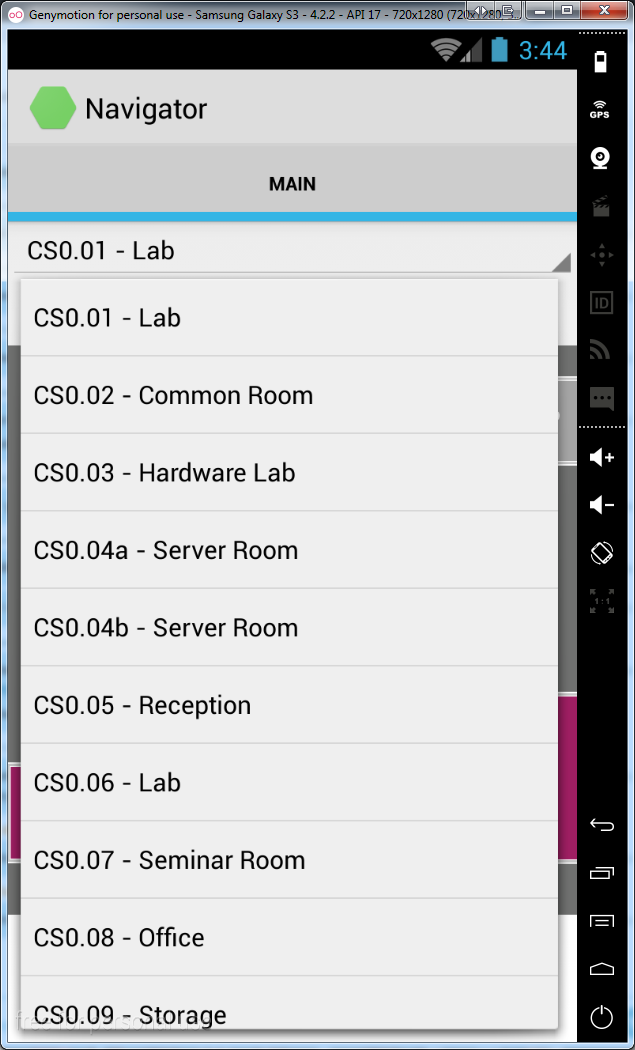
\includegraphics[scale=0.5]{images/search_open.png}
\captionof{figure}{Android room selection menu}
\label{fig:androidSpinner}
\end{center}
        \subsection{Displaying the Floor Plan}
            The vast majority of screen real estate on the main tab of the application is occupied by the image of the floor plan being displayed. Therefore, it was crucial to 
            implement this part of the interface in such a way that it is as simple and intuitive as possible, as the user will spend most of their time using this part of
            the application. By implementing standard features that make use of the touch screen functionality of smart phones (dragging the image around, pinch-to-zoom,
            pressing and holding etc.)
            the learning curve of the interface is greatly reduced as features such as these are extremely common in mobile applications. Therefore, this takes advantage of 
            what can be assumed to be pre-existing knowledge for most end users, reducing the need for excessive tutorials or instructions.
            
            One of the first key issues to handle was the problem that, due to the large size of the floor plan images being displayed (especially when zoomed in), it would need
            to be possible for the for the user to `scroll' through the image. Initially the Android frame \texttt{ScrollView} was used to contain the image. However, it was quickly
            discovered that this only allowed for scrolling in a single direction specified in the AXML code - horizontally or vertically.
            This was clearly insufficient for our purposes, so other methods
            were considered. The first potential fix was that of nesting another \texttt{ScrollView} inside the first, set to scroll in the direction that its parent did not.
            This did allow for scrolling in multiple directions to function, but only one at a time i.e. diagonal scrolling was not possible. In order to solve this problem,
            the Android development team examined various packages, but failed to find one that exactly suited our requirements. Therefore, a custom class
            (\texttt{CustomImageView}) was written to implement all of the desired functionality. This class is described in the section below.
            \subsubsection{CustomImageView Implementation}
                This part of the application is made up of two key classes, one simple, the other more complex. The first of these is the \texttt{CustomImageViewGestureDetector},
                which extends the basic \texttt{SimpleGestureListener} to work with our custom image view and handles the detection of common smartphone gestures. For our purposes,
                we implemented custom detection for touching the screen (known as a `down' gesture), double tapping on the screen, and pressing and holding down on the screen
                (from now on referred to as a `long press').
                
                The main bulk of the new functionality is contained within the \texttt{CustomImageView} class itself. As with all programs that handle image translation and scaling,
                the class contains a matrix that can be applied to carry out translations and zooms on the displayed image (rotations were not required). The class contains functionality
                that allows this matrix to be accessed and applied. Section \ref{subsec:MapMaker} shows this matrix in action when points are translated into correct positions.
                There is also functionality to set the image to be displayed as either a specific bitmap or an Android resource.
                
                The custom behaviours were implemented by monitoring for touch events on the device
                screen. When a touch is detected its coordinates are stored as the position of the `last move'.
                If the `touch count' is at least two (more than one finger is being used, therefore the user is performing either
                a pinch or its inverse), the action was judged to be a scale and the relevant flag was set in the class. If this flag is set, the distance between the two points of contact
                is used to calculate the value by which to scale the image being displayed. This scale is then posted to the image matrix, which is then applied to the image in
                order to carry out the zoom action. Note that if the action would scale the image outside of the bounds specified by the minimum or maximum allowed zoom,
                the scale would stop at these boundary values. Therefore continuing to `pinch' at this point has no effect on the interface. The double tap motion could also be
                used to zoom to the maximum or minimum amount instantly, however this was handled slightly differently. In this case there is no need to calculate a scale
                factor based on movements as the minimum/maximum values are already known. Therefore, the zoom was executed using this known value and the
                (\textit{x, y}) coordinates of the double tap action.
                If the motion was not deemed to be a scale (only one finger is used by the user to perform the motion), the start and end points
                of the movement were used to determine the distance to translate the image in both the \textit{x} and \textit{y} directions. Similar to zooming action, these changes are
                then posted to the matrix and applied to the image in order to scroll in accordance with the user's action. As this took changes in both axes into account, this
                solved the problem of being unable to scroll the view in both directions simultaneously. After any translations/scales were applied to the image, a call was made to
                the \texttt{PostTransitionCutting} function. This applies the transitions to the local version of the image matrix and handles edge cases where the image may overflow
                or underflow the view. Once this process is complete, the local image matrix is then updated. The final custom behaviour handled was that of the long press. When a 
                long press is detected, a \texttt{LongPressHandler} is executed. In our case, a long press creates a menu that allows the user to specify a start or end location
                directly on the floor plan image, should they not wish to use the drop down menu. This menu is created by creating an \texttt{AlertDialog} object which asks the
                user whether they wish to place a start point or an end point on the floor plan (The debugging version of the application also allows the user arrow to be placed
                in order to facilitate testing). This menu is shown within figure ~\ref{fig:androidStartEndMenu}. Once the choice has been made, the relevant coordinates are stored and used to draw the new points - section \ref{subsec:MapMaker}
                explains the drawing process in detail.

                    
\begin{center}
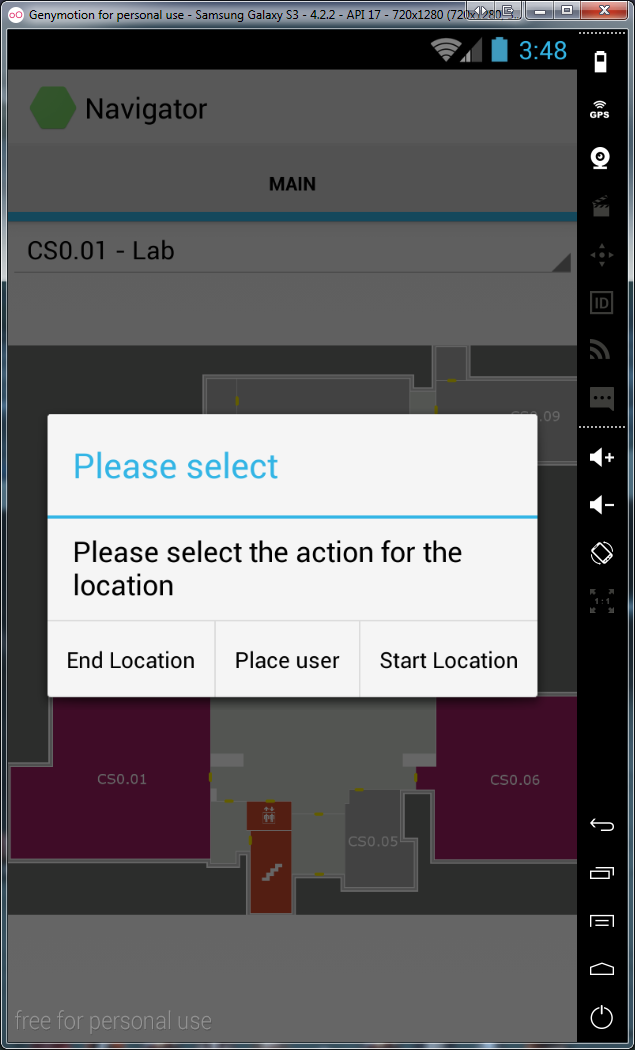
\includegraphics[scale=0.5]{images/location_action.png}
\captionof{figure}{Android start and end point selection menu.}
\label{fig:androidStartEndMenu}
\end{center}                    
                                    
                
        \subsection{Managing Points and Paths}
            Once the image was being displayed correctly and could be interacted with as required, the next step was to facilitate the drawing of start points, end points, the user location,
            and the path to follow on the screen. There were two approaches considered for this, the advantages and disadvantages of which are discussed below.
                \subsubsection{Overlay Based Approach}
                    This was the first of the approaches to be considered and involves the creation of a separate view to display the start/end points, user arrow, and path on top
                    of the floor plan image. Initially, this was an attractive solution as it allows the program to be constructed in a more modular way, keeping the management of the
                    floor plan apart from that of the drawing. However, it also introduces the additional task of managing the overlay itself. This becomes particularly challenging
                    when the user is scrolling around the floor plan or zooming in and out, due to the necessity of ensuring that the overlay view is also adjusted accordingly.
                    The other downside is that translating point coordinates from the overlay may also be tricky, perhaps requiring the use of another transformation matrix.
                    In the end, this method was deemed unsuitable for our purposes, so another solution was considered: directly editing the bitmap being displayed in the
                    \texttt{CustomImageView}.
                \subsubsection{Direct Bitmap Editing Approach}
                    This method involves editing the actual image being held in the image view. This approach addresses the primary issues found with the overlay based solution:
                    handling situations where the user wishes to either move or scale the floor plan by drawing the additional shapes into the bitmap image.
                     In this case, as the points and/or lines are part of the image itself, any translations
                    or scalings applied to the image as a whole will also, by extension, affect the points and lines. The downside to this approach is that it requires the image to be reset
                    to the default resource any time that a previously drawn point must be removed (such as moving a start point to a different location, or any movement of the
                    user arrow). It was thought initially that this may be a significant issue that could introduce a noticeable delay into interface updates, something that is clearly
                    unacceptable when a pleasant user experience is a key objective. Fortunately, some brief testing (on both emulators and physical Android devices)
                    revealed that this was not the case; there was no noticeable delay in interface updates. Following this discovery, it was decided to adopt this strategy instead of the
                    overlay system. The following section details how our custom helper class, \texttt{MapMaker}, handled the drawing of the required graphics.
                \subsubsection{MapMaker Helper Implementation}
                    \label{subsec:MapMaker}
                    The \texttt{MapMaker} class was created in order to keep the implementation of this part of the program separate from the rest of the application, in keeping
                    with the modular structure of most object-oriented programs. This meant that this module could be tested, maintained, and developed independently without 
                    adversely affecting the main activity -provided that changes to internal code did not alter the external behaviour of the class beyond what was intended.
                    
                    The first key component of this class was specifying the bitmap options that were applied to all of the decoded bitmaps (these being the plain floor plan,
                    the floor plan with the graph grid shown, and the user arrow).
                    The dither option is set to true in order to reduce noise in the image, in an attempt to prevent issues such as colour
                    banding. The bitmaps are also set to be purgeable i.e. the system can reclaim the memory used if absolutely necessary. In later versions of Android, this flag
                    is ignored, but enabling it allows a greater degree of backwards compatibility. Also note that enabling this did not prevent all memory issues, which will be discussed
                    later. The final key option was ensuring that the image is mutable. This is important as only mutable bitmaps can be used with Android
                    \texttt{Canvas} functionality, which enables the editing of the image i.e. only mutable images may be drawn into. In older versions, images could only be
                    made mutable by copying them, however this is inefficient in terms of both computation and memory, and is no longer the case for these very reasons.
                    
                    Upon initialising the instance of \texttt{MapMaker}, the class decodes and stores three android resources, all of which are bitmap images. These are the plain
                    floor plan, the floor plan with pathfinding grid, and the arrow used to display the current position of the user. The class provides functionality to clone
                    all of these bitmaps, which prevents the need to re-decode the images should a new blank copy of the image be required (such as when re-drawing the map
                    when erasing a point). This is beneficial performance-wise as decoding can be a slow process. As this redrawing has the potential to occur very frequently,
                    achieving good performance was of the utmost importance.
                    
                    Resetting the map was a simple process. When a call to \texttt{ResetMap} is made, a check is made to see if the grid is currently being drawn or not. Depending
                    on the result of this check, the correct bitmap can be cloned, edited, and then finally set as the current image being displayed by the view.
                    This function also makes sure to to call \texttt{Recycle} on the old bitmap image in order to ensure that the memory that it occupied is properly freed and
                    returned to the system at the next execution of garbage collection.
                    
                    Drawing into the bitmap was more complex, however. The bitmap is redrawn in the following situations:
                    \begin{itemize}
                        \item New start/end point selected.
                        \item User has taken a step, therefore the arrow must be moved.
                        \item The path must be (re-)drawn for some reason.
                    \end{itemize}
                    When a new start/end point is selected, the coordinates of this point are translated to coordinates in the bitmap via a transformation matrix
                    (discussed later in this section) and then stored within the \texttt{MapMaker}. Following this, a call is made to \texttt{DrawMap}, which first resets the
                    image (using \texttt{ResetMap}). Following this, the application forms a \texttt{Canvas} from the fresh image in order to facilitate the drawing of the
                    required shapes. Once this has been done, some simple checks are carried out in order to determine whether any start/end points are currently set.
                    If this is the case, the points are drawn at the previously stored coordinates using the \texttt{DrawCircle} function within \texttt{Canvas}. A similar check
                    is used to see whether the user arrow must also be drawn, if it must, the user arrow bitmap is also drawn into the \texttt{Canvas} by making use of
                    \texttt{DrawBitmap}. If both start and end points have been set, then the user path must also be drawn. Firstly, the correct nodes in the graph are obtained
                    by using the \texttt{FindClosestNode} function implemented within the \texttt{PathfindingGraph} object. These points are then passed to
                    \texttt{FindPath} in order to determine theh path to draw. Once the sequence of points has been calculated, the program iterates over this list, drawing lines
                    between adjacent points within the list using \texttt{DrawLine} until the end of the path is reached. Once all of the drawing has been completed, the
                    \texttt{Canvas} is disposed of in order to free memory. Finally, the image being displayed by the custom image view is updated to the newly edited
                    version.
                    
                    The final functionality that had to be added to this helper class was the ability to translate the coordinates of the location that a user has touched on the screen
                    into correct coordinates within the bitmap image. This was necessary due to the need to be able to place start and end points at a location specified by the user
                    performing a long press on the map via the device screen. The function takes either (\textit{x, y}) coordinates or a two-dimensional vector as input, and returns a
                    two-dimensional vector containing the newly translated coordinates. This is implemented by obtaining the image matrix from the custom image view and calculating
                    the inverse of this matrix. This new matrix can then be applied to the inputs in order to return the correctly translated coordinates. Figure  ~\ref{fig:androidPathDrawing}  shows the Android path drawing.

\begin{center}
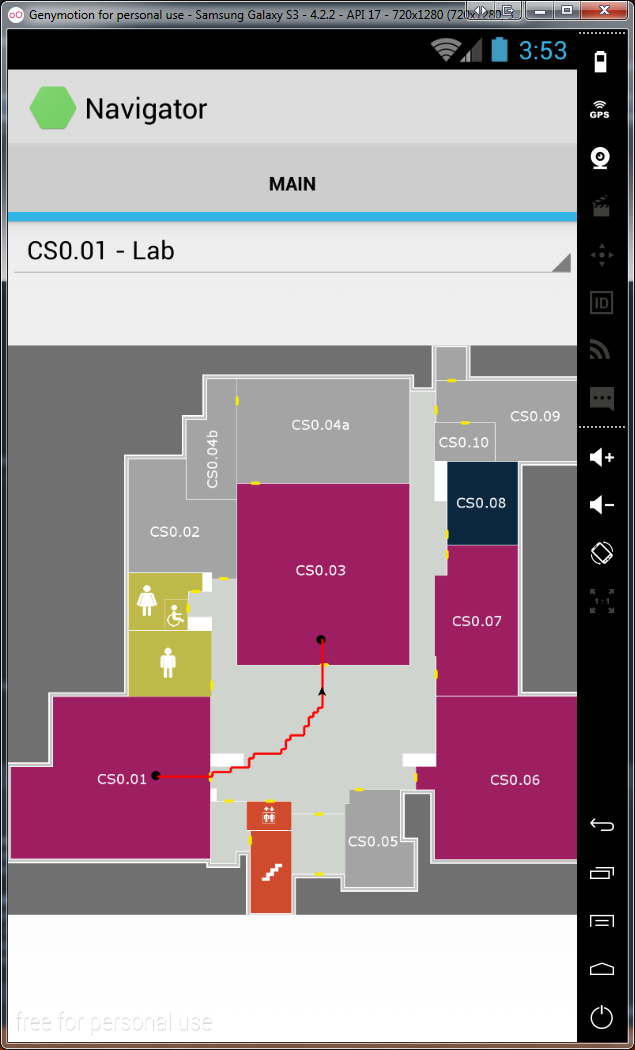
\includegraphics[scale=0.5]{images/pathfinding.png}
\captionof{figure}{Android path drawing.}
\label{fig:androidPathDrawing}
\end{center}

\section{Android Development}
    \subsection{Accessing Android Sensors}
        In order for the step counter to function, it was necessary to pass it the readings from various device sensors. As this cannot be handled in the shared
        project code, native Android code was developed to facilitate this process. This section explains the implementation of this part of the application. As
        mentioned previously, the main sensors used are the accelerometer and the compass, in order to obtain acceleration and heading values, respectively.
        The events fired by the sensor reading classes are handled in the main activity, which passes them to the shared code \texttt{Collision} class for processing.
        \subsubsection{SensorProcessorBase Implementation}
            The first custom class implemented for the purpose of managing the access to the Android sensors was the abstract class
            \texttt{SensorProcessorBase}. This class was later extended by the classes \texttt{Acceleration} and \texttt{Rotation}, discussed
            later on in this section. This abstract class is responsible for providing the following functionality:
            \begin{itemize}
                \item Storing a list of sensor types its child class is responsible for.
                \item Storing the time since the last sensor reading.
                \item Specifying a reading delay (how often we want to be able to access the sensor).
                \item Storing a sliding window of previously read sensor values.
            \end{itemize}
            Implementing the list of accepted sensor types is a simple matter of adding the relevant pre-defined sensor types to the list that was created. For example,
            the accelerometer would add the value \texttt{SensorType.Accelerometer}. This allows each instance of a sensor class to filter out values that it does not
            require by simply ignoring them.
            
            Accessing the time of the last sensor reading was also a fairly simple matter. Whenever a new reading is taken, the current time
            is stored within the class. Therefore, if the time since the last reading is requested, it is a simple matter of returning the value of the current time minus the stored
            value for the time of the previous reading. This function is primarily used when determining whether a change in the value of a sensor needs to fire the associated type
            of event. When a sensor value is changed, the function that handles this new value is only called in the case where the time since the last reading is not less than that
            of the specified reading delay, therefore allowing the amount of sensor updates to be limited to a desired rate.
            
            The final piece of key functionality in this class, the history of previously read values, is implemented through the use of a \texttt{FixedSizeQueue}. This a custom
            type implemented in shared code that stores a set of values in first-in, first-out order. If a new insertion would increase the size of the queue above the specified
            capacity bound, the oldest item is subsequently removed from the data structure. In this manner, a sliding window of previous sensor values can be stored by simply
            adding each new reading to the implemented queue, which will handle the removal of old data when capacity is reached, thereby keeping the window at the specified size.
            In our case, we chose to store the ten most recent sensor readings, though this amount could be easily changed if it later became necessary.
        \subsubsection{CustomListener Implementation}
            The next part of custom implementation was a rather simple piece of code called the \texttt{CustomListener}. This was essentially a wrapper class for the 
            Android \texttt{SensorManager} that allowed for access to both the \texttt{Rotation} and \texttt{Acceleration} classes through a single object instance. This
            was primarily done for code modularity, readibility, and ease of extension.
            
            The first of the added methods, \texttt{OnAccuracyChanged}, contained no code as we did not need to handle any changes to the precision of the sensors being
            used. However, leaving it in as a stub would allow for behaviour to be added easily, if it was later deemed necessary to be able to adjust the accuracy of
            a sensor. For example, an extension could potentially examine the effects of sensor accuracy on step detection or heading inference.
            
            The second method added to this class was an event handler for when the value of a sensor changes i.e. a new reading is returned. Intuitively, this method
            is named \texttt{OnSensorChanged}. This method takes the input sensor event and passes it to the handlers in both \texttt{Acceleration} and \texttt{Rotation}.
            This is necessary due to the values of certain sensors being required by both classes, these sensors being \texttt{Gravity} and \texttt{MagneticField}. This requirement
            further supports the integration of both sensor types into this wrapper class, \texttt{CustomListener}. If they were not kept together, handling this overlap of 
            required sensor readings would require each instance to be handled separately, a solution far less clean than the one provided here, in terms of both performance and
            maintainability.
        \subsubsection{Acceleration Class Implementation}
            This class (\texttt{Acceleration}) is responsible for accessing the accelerometer of the Android device being used and, therefore, is also responsible for calculating
            the final acceleration vector (a 3-tuple in this case) and returning this vector upon request. The inital setup of an instance of this class first adds 
            the sensor types \texttt{Accelerometer}, \texttt{MagneticField}, and \texttt{Gravity} to its list of accepted sensor types. This allows the instance to filter out
            unnecessary values, as discussed prior. Following this, the reading delay is set to a value of ten milliseconds, thus one hundred sensor readings are taken per second.
            More than this value
            leads to too many events being fired, whereas less was found to be detrimental to step detection.
            
            The remaining functionality of this class is found in \texttt{SensorChangedProcess}. This is the method called from the \texttt{CustomListener} in order to access a new
            acceleration value. It firstly carries out a check to determine whether or not the input sensor event is required by the class i.e. whether it is one of the sensor types previously
            added to its list of accepted types. If this is indeed the case, the values are converted into array form and stored within variables for later use. If not, the event can
            be ignored. Once this process is complete, the method checks whether it has the necessary values to compute a valid acceleration value. If it does not, the method 
            simply returns. However, if a value can be calculated, this is done as follows. Firstly, a rotation matrix is calculated using the \texttt{SensorManager} and the
            values for \texttt{Gravity} and \texttt{MagneticField}. This matrix is then inverted and multiplied by the acceleration vector in order to determine the actual
            acceleration vector in world coordinates. This value is then stored in the value history for the class, and then subsequently fired as a \texttt{ValueChanged} event.
        \subsubsection{Rotation Class Implementation}
            The heading obtained from the phone's compass is used as the direction of the user's motion whenever a step is detected. More specifically, this heading corresponds to the azimuth reading which is defined to be the angle between magnetic north and the phone's Y-axis~\cite{azimuthDefinition}. In iOS, this azimuth reading along the device's world axes is readily available through the `CLLocationManager' class which performs all the necessary pre-processing. The equivalent in Android's API was the software-based `Orientation' sensor which made use of the physical accelerometer and magnetometer sensors to directly provide the azimuth. However, the sensor was deprecated in API Level 8 and cannot be used for this purpose any longer. 

The current recommended approach in the documentation to compute the azimuth value is to manually instantiate the gravity and magnetometer sensors and use their readings (after low-pass filtering to compensate for noise) to perform the necessary calculations~\cite{ENU}. This involves using the readings to obtain the rotation matrix, which is then passed to the `GetOrientation' method in SensorManager that returns the azimuth value. Note that the SensorManager's `RemapCoordinateSystem' method is used on the rotation matrix before passing it to GetOrientation to obtain the azimuth reading along the world axes.  

On implementing this method it was found that the azimuth value obtained was not responsive enough - there was a considerable lag between the user changing orientation and this being reflected in the azimuth value. Furthermore, rotating the phone along any of its axes resulted in a considerable change of this value in spite of using RemapCoordinateSystem for transformation to world axes in the manner suggested in the documentation. Both these shortcomings meant that the azimuth value could potentially be wildly inaccurate at the time a step is detected, which makes this approach of computing user heading unsuitable for use with the navigation system. 

An alternate method proposed by Nguyen, H. on Stack Overflow~\cite{azimuthFinal} was found to give far better results, albeit with certain restrictions. This approach once again utilises the gravity and magnetometer readings to compute the rotation matrix. Assuming that the phone is held in portrait mode with its Y-axis facing upwards, the heading of the user can be calculated using the direction of the phone's back camera with respect to magnetic north. This direction is obtained in radians by taking the arctangent of the second and fifth elements of the rotation matrix. In order to deal with fluctuations due to noise a fixed-length sliding window of previous rotation matrices is maintained. All these rotation matrices are averaged together to give a single matrix which is used to obtain a stable value of the current direction.

As the heading in this approach is defined only when the phone is held upright in portrait mode, this heading value is manually set to be undefined whenever the phone is held flat. Such situations are detected by observing the angle between the device's Y-axis and the world XY plane, obtained by taking the arccosine of the 8th element of the rotation matrix. The device is defined to be flat if this angle is either lesser than 25 or greater than 155 degrees and hence the heading is computed only when the phone is between these angles.

\section{iOS Development}


\subsection{Building an iOS application}

There are several things that are needed to build a working iOS application. iOS applications work using the Model View Controller (MVC) design pattern. This attempts to separate the interface of the application (views) from the inner workings and data stored (model) with communication between these two components being moderated by a separate class (controller). Each class created in an MVC application should ideally fall under one of these categories. 

\subsubsection{Model}

In an MVC application, the model is designed to encapsulate the problem-domain and internal logic of the application. That is, it is responsible for generating, storing and processing the information that is related to the application. It is also responsible for any data access including web access and communicating with an external storage system such as a database. A simple diagram of an MVC architecture is shown in image \ref{MVC}. The application logic and data access sections of the model should not be aware of the inner workings of each other in order to provide flexibility when changing the type of data storage or the application logic. 

\subsubsection{View}

The view is the part of the application that shows the various components and data on the screen for the user to see. It is also responsible for providing the necessary components that can allow the user to interact with the application. The view is additionally responsible for presenting any data given to it in a human readable way, such as presenting it in a graph or pie chart or in a listed table. In iOS, views are created with the use of the storyboard feature that is described in more detail below.

\subsubsection{Controller}

The controller is the final piece of the application that links the views to the model. The controller is primarily what the user interacts with whenever they interact with the application. While the view is responsible for showing any inputs such as buttons and text fields, it is the view controller that converts these into commands which are passed down to the model. Similarly, any information returned by the model is converted into the proper format by the controller and given to proper view in order to show. In a way, the controller is the glue that binds both the views and the models together and there should be no communication between the two that does not go through the controller at some point.

\begin{figure}[]
\centering
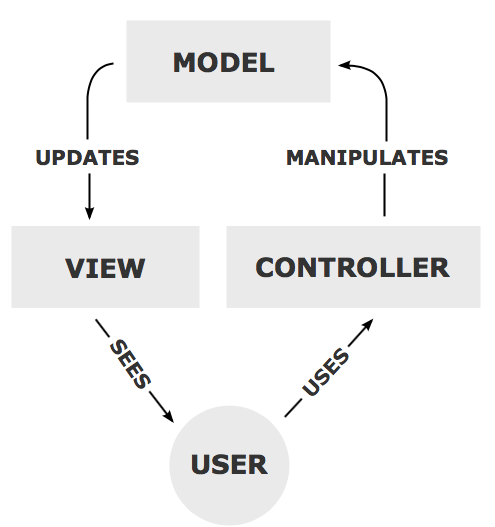
\includegraphics[width=0.5\textwidth]{images-implementation/MVCLayout.png}
\label{MVC}
\caption{Diagram showing a simple flow chart of an MVC application. Image obtained from \cite{mvc}}
\end{figure}


\subsection{Storyboards}
One of the other most important concepts in iOS development is storyboards. Storyboards work as a view designer and transitioning controller between different views. They provide the hooks through which a controller can process inputs and tell the views what and how to interact with the user. Storyboards are an iOS specific feature and typically require the use of Apple's Xcode development platform to view and edit. However, Xamarin has their own version of the storyboard editor that provides some support for C\# based coding and is easier to use to hook visual components into the C\# code in the view controller.

\subsection{APIs}
iOS provides a vast host of APIs that are ideal for a large number of tasks such as displaying information and resources, as well as accessing on-device data such as accelerometer and gyroscope data. Apple’s original iOS APIs are available as C\# libraries under the Xamarin framework and are very similar in structure and usage to the original Objective-C and Swift versions. These APIs are designed to be as easy to implement as possible and this was really seen during development when compared to Android development as certain functionality and sensor readings was seen to be much more easily accessible in iOS. Additionally, much of the functionality follows a very strict hierarchical inheritance structure which lends its hand to many scenarios such as creating a complex view. All iOS visual components inherit from the UIView class, of which a component of this is a collection of UIView named subviews which are rendered within relation to the parent UIView. This effectively allows a hierarchical structure of UIViews which can be rendered and set dynamically. UIView classes also have the added functionality to automatically redraw whenever a change is made with them, as long as this call is made on the main UI thread. This structuring, alongside the simplistic nature of the components and their ease of creation, modification and rendering, makes it incredibly easy to create complex applications from just a few simple boiler plate components.

\subsection{Development}

Our development for an iOS application started with creating a simple blank Xamarin cross platform solution for Android and iOS. This provides 3 separate projects in which we can work with. There is 1 project each for the different mobile platforms and a 3rd project that acts as the standalone shared code that can be accessed by both iOS and Android. Due to the nature of this, the shared code project must be written independently from any specific platform and cannot use or rely on libraries or functionality that are specific to a single platform.

\subsubsection{Storyboard and Interface}
We start off with a single storyboard for iOS simply titled main.storyboard. From here, we built the visual end of the iOS application and determined how many different screens (views) we were going to have and how to transition between them. We decided to only go with one storyboard since there were not going to be many screens and the transitions between them would be simple and would use pre-made segues (transitions in iOS). We start simply with a Navigation Controller. A Navigation Controller is a class that is responsible for controlling a hierarchical navigation of different screens as seen in many native iOS applications.

\begin{figure}[]
\centering
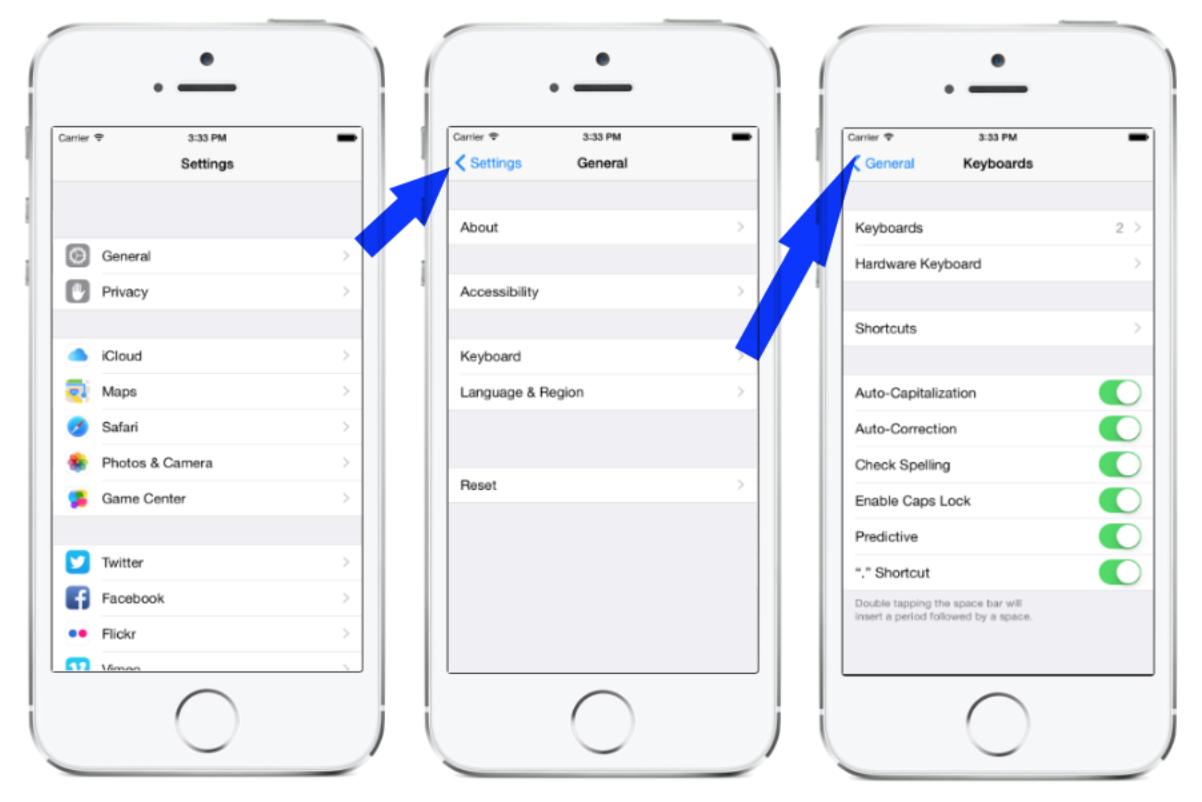
\includegraphics[width=0.5\textwidth]{images-implementation/NavigationController.png}
\label{NavigationController}
\caption{Image showing the workings of the Navigation Controller component in iOS .Image obtained from \cite{iosnavigxtioncontroller}.}
\end{figure}

A Navigation Controller is able to keep track of the visited screens and the path that the user has taken through them and allows the user to back-track through the application. We initially use this to create an options screen which could linked to from a button on the title bar of the main screen shown in image \ref{initStoryboard}. The Navigation Controller then automatically creates the back button on the options page. This can allow for a complex hierarchical structure that is easily controlled and changed.

\begin{figure}[]
\centering
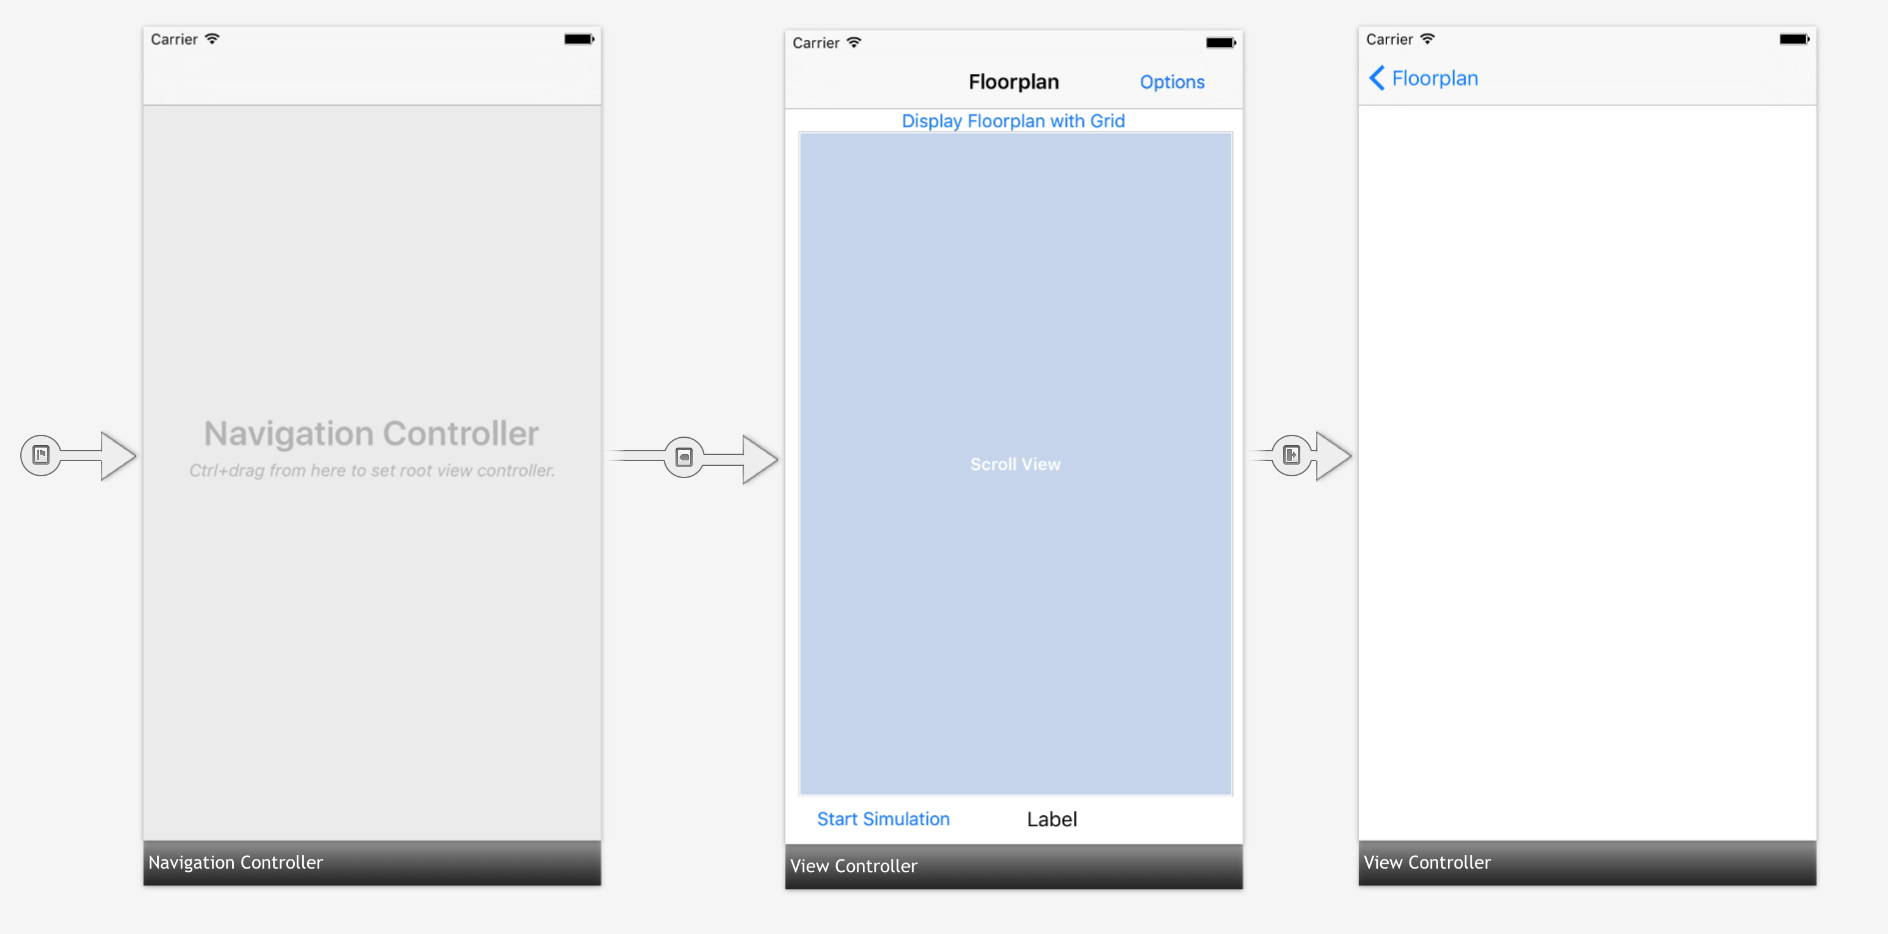
\includegraphics[width=0.5\textwidth]{images-implementation/InitialStoryboard.png}
\label{initStoryboard}
\caption{Screenshot showing a early design for the main storyboard. The Navigation Controller and its derived navigation controls can be seen in the title bars for the different screens shown.}
\end{figure}

The main map view was implemented using a UIScrollView class. This would allow us to show an image which could be panned and zoomed, as well as respond to additional gestures on top. Since UIScrollView is able to display any UIView class, this allows us to display many views that will pan and zoom together by wrapping them in a UIView wrapper. Since the map images and other components were going to be loaded dynamically, they had to be set manually in the view controller rather than in the storyboard editor. To achieve this, we needed a hook to the scroll view in order to set the contents dynamically in the view controller. This is a very simple procedure in Xamarin and simply involves giving the component a name. Doing so will create a hook in the ViewController.designer.cs class which is a partial class of ViewController.cs. This allows us to reference the scroll view and set up the contents and properties accordingly from within the View Controller. This is described in detail in the View Controller section.

We decided to implement a search functionality to allow users to search for the room they are looking for. This would then allow them to select whether to set their location to that room, or to set that room as a destination for navigating to. To do this, we added 2 new components to the main view of the application; a search bar and a search results/prediction table. These components can be seen as storyboard components in image \ref{IOSRoomSearchInStoryboard}. As part of our implementation for representing the floor plan, we also had a list of all the rooms contained by the map. This was implemented using a custom controller called CustomSearchController.cs and the search bar and table view were hooked into the View Controller in the same way that the scroll view was. This class would take references to the search bar and table view components, as well as a list of the rooms obtained from the floor resources. All logic pertaining to the search functionality was then performed in this class and other classes referenced by it, this allowed us to separate out certain functionalities from the main view controller. A working version of the room search functionality can be seen in image \ref{IOSRoomSearchInApp}.

\begin{figure}[]
\centering
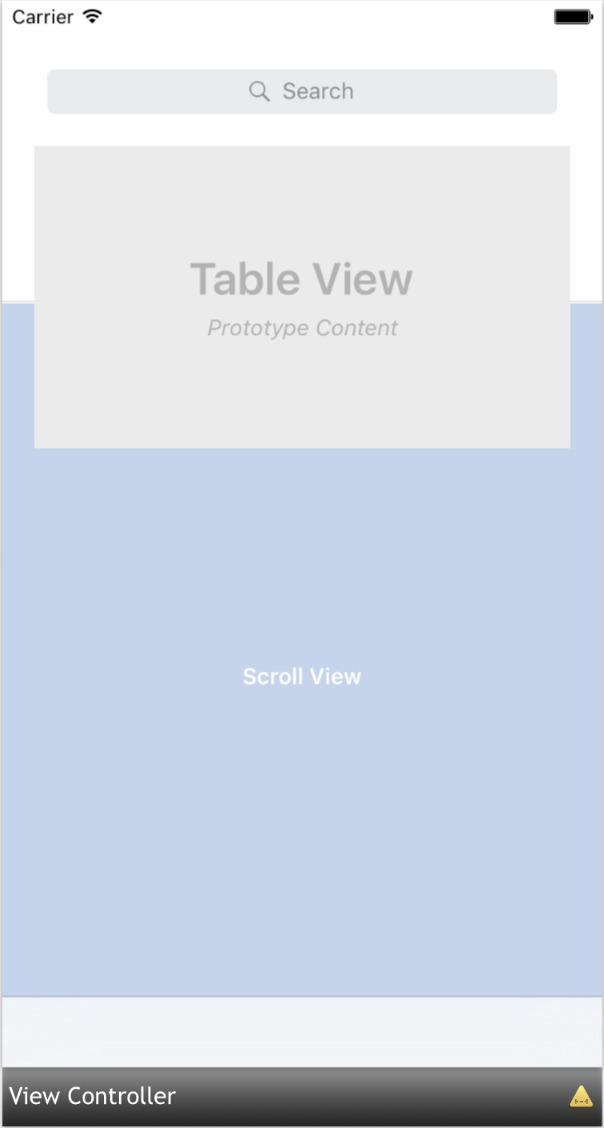
\includegraphics[width=0.5\textwidth]{images-implementation/IOSRoomSearchInStoryboard.png}
\label{IOSRoomSearchInStoryboard}
\caption{Screenshot showing how the search bar and result/prediction table are shown in the main storyboard.}
\end{figure}


\begin{figure}[]
\centering
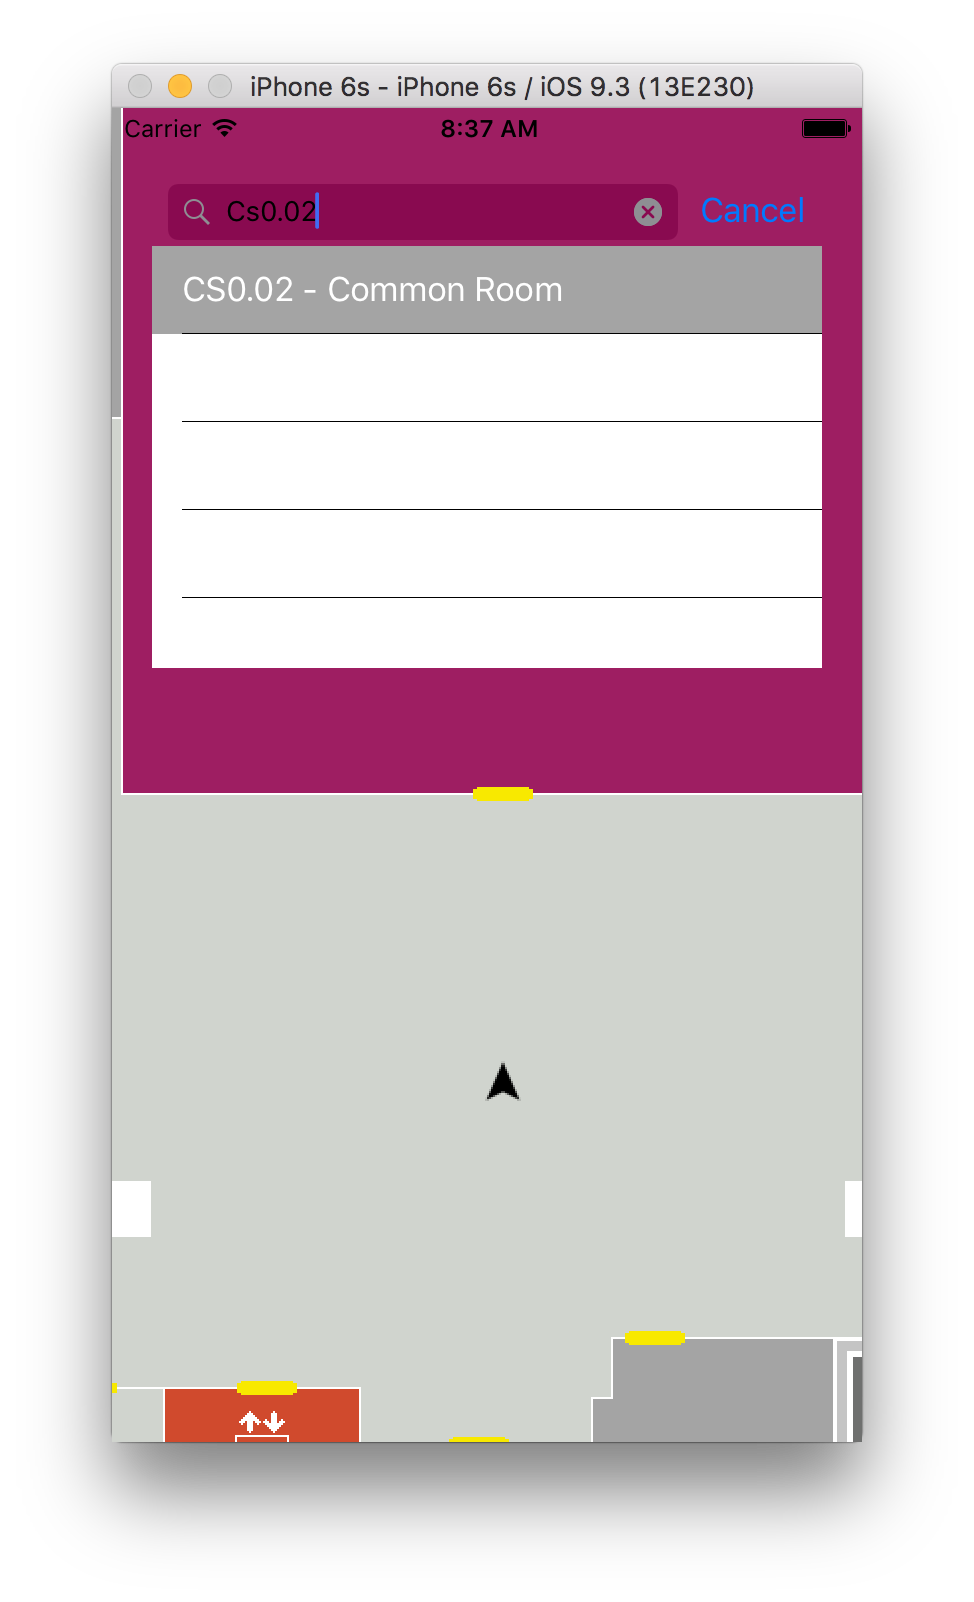
\includegraphics[width=0.5\textwidth]{images-implementation/IOSRoomSearchInApp.png}
\label{IOSRoomSearchInApp}
\caption{Screenshot showing how the search bar and result/prediction table are shown in the application.}
\end{figure}

\subsubsection{View Controller}
The ViewController.cs file is where the majority of the iOS specific code is kept. It is responsible for delegating all communication between the view components and the model of the application which was kept in the shared code project. It was also responsible for assigning many of the dynamic variables and properties of the view components that could not be simply created using the storyboard editor. Because of this, the view controller class is one of the longest, most feature heavy classes that is present in the application. One of the primary goals at the beginning of the project was to be able to get a simple view of a map on the screen that could be panned and zoomed by the user. We achieved this primarily with the use of a UIScrollView class. The initial scroll view component was placed using the storyboard editor, however since we wanted the image displayed to be able to be loaded dynamically to facilitate changing maps, we could not set the contents or any derived properties (such as content width and height) from the storyboard editor and instead had to elicit the use of the view controller class. An object hook was placed so that we could refer to the scroll view from inside the view controller and the following code was used to import and display the map.
\begin{lstlisting}
floorplanImageNoGrid = 
	UIImage.FromBundle("Images/FinalDcsFloor1.png");
floorplanImageView.Image = floorplanImageNoGrid

floorplanScrollView.AddSubview(floorplanImageView);
floorplanScrollView.ContentSize = floorplanImageNoGrid.Size;
floorplanScrollView.ViewForZoomingInScrollView += 
	(UIScrollView sv) => { return floorplanImageView; };
\end{lstlisting}
The first 2 lines of this code segment simply loads the proper map image from the applications resources and assigns it to a UIImageView class in order to be able to interact with other UIView classes. The 3rd line then adds this subview to the scroll view which is already set to display on the screen. The 4th and 5th lines are included in order for panning and zooming to work correctly. This simply set the contained size of the scroll view to be equal to that of the image view and the scroll view is told to zoom the image view when pinch-to-zoom gestures are registered. This code segment was included as a simple example to show how easy it is to include and manipulate visual components with ease in iOS. While this is a simple example, the main concepts of a hierarchical architecture of UIViews will remain for the remainder of this section. It is important to note that a UIView can contain more that one subview.

The next step in creating a usable navigation app is to be able to draw things on the map such as the user's location and the path to their destination. Here we can utilise the structuring of UIViews by creating a container view. This is an effectively invisible view that essentially encapsulates 2 or more subviews into one container that can be acted upon and changed as a single entity. By creating a container view with the map image and a user's location arrow image as subviews, we can instruct the scroll view to act upon the container view instead of either of the subviews. This results in the scrollview being able to pan and zoom both views simultaneously to create seemingly one picture. 

\begin{lstlisting}
container.AddSubview(floorplanImageView);
container.AddSubview(userLocationArrow);
container.SizeToFit();

floorplanScrollView.ContentSize = container.Size;
floorplanScrollView.ViewForZoomingInScrollView += 
	(UIScrollView sv) => { return container; };
\end{lstlisting}
While this works nicely, we noticed that on many existing mapping applications such as Google and Apple Maps, the user location arrow did not scale with the map when zooming. Instead it stayed at a constant size and simply stayed to reflect the correct location. This was unfortunately not as simple a change as you might expect. By changing the floowplanScrollView.ViewForZoomingInScrollView property to return just the map UIImageView, we ran into the problem that the user location arrow could not distinguish between the absolute coordinated on the map and the relative coordinates to the container view. This effectively meant that as the view was scrolled in and out, the relative position of the arrow on the map would increase and the map images coordinate space was compressed. The easiest solution we could find to this problem was to manually recalculate and modify the location arrow coordinates in relation to the zoom factor of the scroll view.


[image of incorrect location arrow zooming]
[image of correct location arrow zooming]

\subsubsection{Paths}

The second part that needed drawing over the main map was the actual path to the user's destination. iOS supplied a useful CGPath component that could draw a customised line between a set of points on a 2D space. However, in order to be compatible with the other UIView based components, we had to create a custom PathView.cs class that would act as a wrapper to the CGPath class. This class would be responsible for drawing the path and ensuring it remains consistent with the map image during zooming. It would also contain additional methods for encapsulating the CGPath object from the outside and for adding and getting points on the path in an abstracted way. 

In order to interact with the map, we implemented a gesture recogniser on the scroll view. This allows for a long tap and hold on any part of the image and would result in a popup that would allow the user to set the point as either a start or and end point for a path. Setting a start location would move the user to that particular point, while setting an end location would attempt to draw a path from the user to the destination. Creating this was fairly simple and simply required the use of the UIAlertController class which allowed us to create iOS style alerts with customisable options. An image for a preliminary options sheet is shown in image \ref{IOSAlertSheet} and the code is shown below.

\begin{figure}[]
\centering
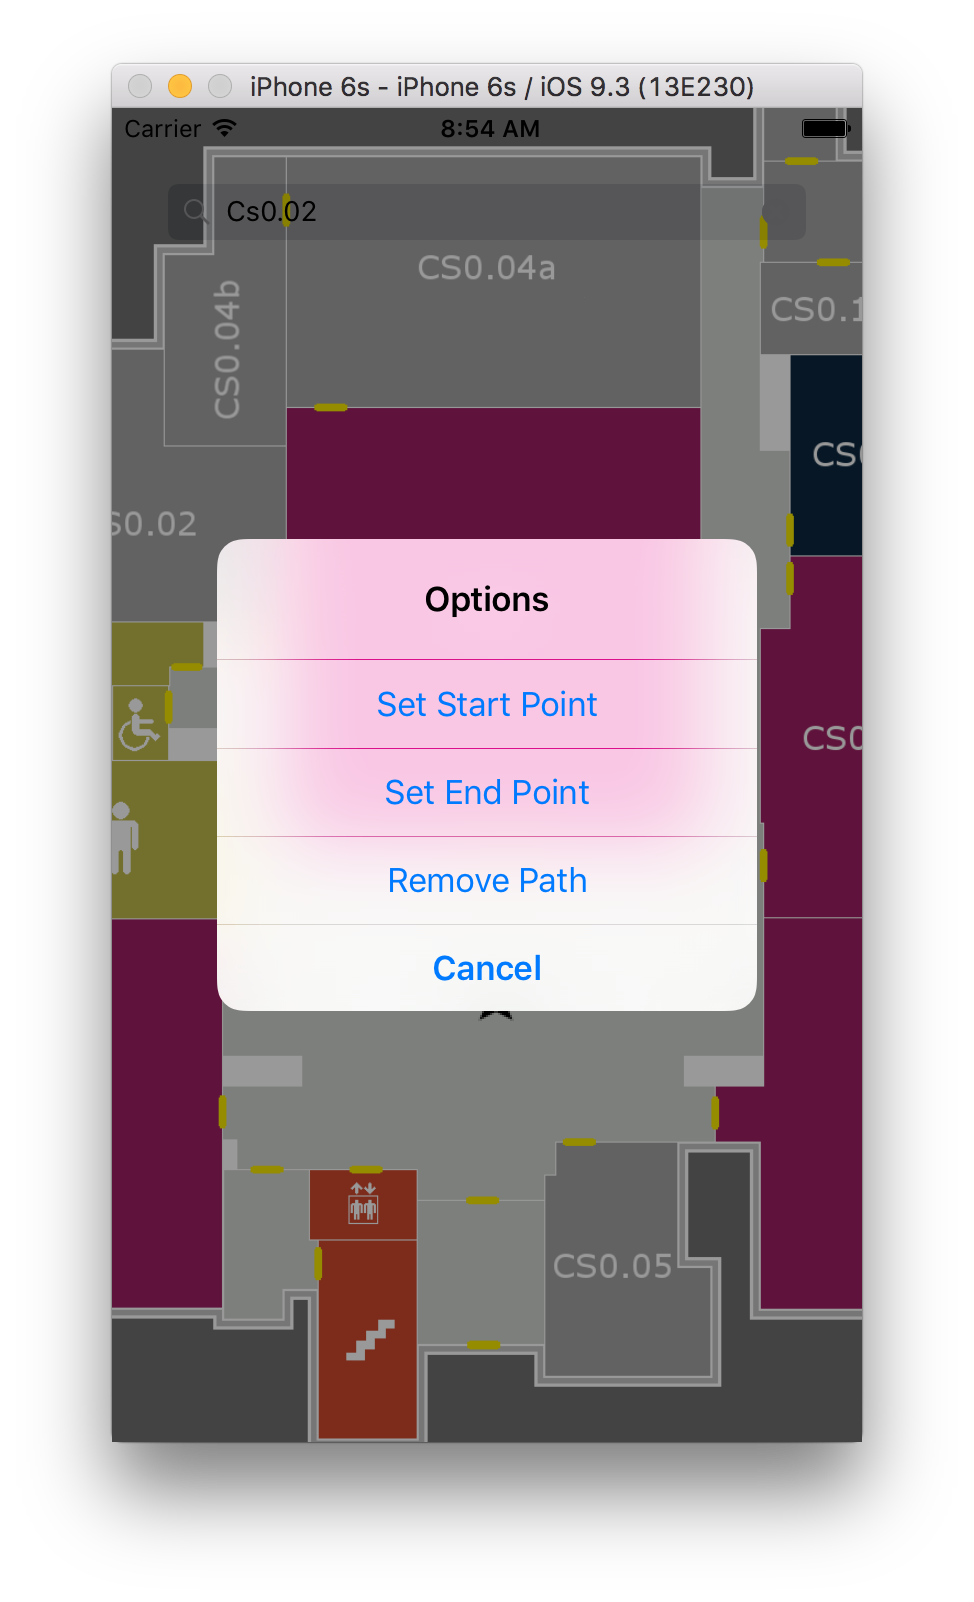
\includegraphics[width=0.5\textwidth]{images-implementation/IOSAlertSheet.png}
\label{IOSAlertSheet}
\caption{Screenshot showing the iOS alert sheet that would show when long pressing an area on the map.}
\end{figure}

\begin{lstlisting}
// Create a new Alert Controller
UIAlertController actionSheetAlert = UIAlertController.Create(
	"Options", 
	null, 
	UIAlertControllerStyle.Alert
);

// Add Actions
actionSheetAlert.AddAction(
	UIAlertAction.Create("Cancel",
	UIAlertActionStyle.Cancel, 
	null));
actionSheetAlert.AddAction(
	UIAlertAction.Create("Set Start Point",
	UIAlertActionStyle.Default, 
	(action) => setStartPoint(tapX, tapY)));
actionSheetAlert.AddAction(
	UIAlertAction.Create("Set End Point",
	UIAlertActionStyle.Default, 
	(action) => setEndPoint(tapX, tapY)));
\end{lstlisting}

\subsubsection{Getting Sensor Values}
One of the crucial aspects required for the step detector and wall collision classes to work was various device sensor readings. These included heading information and accelerometer and gyroscope values. Since these classes were designed and written as shared code to be utilised by both iOS and Android, they could not directly access these sensor readings themselves and instead had to implement methods for receiving these from the correct native projects. As such, sensor readings were the responsibility of the native projects to collect and manipulate into the correct format required by the step detector and wall collision classes. Retrieving sensor readings in iOS is fairly simple and many similar sensor readings are nicely encapsulated into easy to understand objects. Additionally, the Xamarin iOS framework makes use of the functional paradigm support of C\# in order to simplify the process of receiving updated sensor values. C\# is able to handle functions as first order variables, and as such, they can be easily passed into functions as arguments and can be dynamically run by variable name. This allows us to pass our handler functions into the sensor managers, that is, the code that will be run whenever a new set of updated values is provided. This allows easy encapsulation and purity of the sensor managers and a relatively simple solution to retrieving updated values, an issue that could potentially require a much more complex solution with other languages. To demonstrate this, we will show how accelerometer readings, which will be crucial for step detection, are taken on an iOS device using Xamarin and C\#. The method definition for retrieving accelerometer values is 
\begin{lstlisting}
CMMotionManager.StartAccelerometerUpdates(
	NSOperationQueue queue, 
	CMAccelerometerHandler handler
);
\end{lstlisting}
The important argument here is the CMAccelerometerHandler handler. This is where the method that is called whenever the accelerometer values are updated. The CMAccelerometerHandler referenced here is a delegate type. A delegate is a special keyword used by C\# to specify a method definition without actually specifying any actual body to the method. The declaration for CMAccelerometerHandler is shown below.
\begin{lstlisting}
public delegate void CMAccelerometerHandler (
	CMAccelerometerData data, 
	NSError error
);
\end{lstlisting}
What this declaration does is define a type of method CMAccelerometerHandler that takes those two particular arguments. Now any event that is created with the type CMAccelerometerHandler will require its subscriber methods to also implement this same declaration. This ensures that the correct arguments can be passed into the subscriber methods when the event is called. Shown below is the implementation used in our application for retrieving accelerometer values and passing them into the step detector class. In this example, we make use of an anonymous lambda function instead of declaring a full named method. As such, this lambda function has the same declaration as the CMAccelerometerHandler delegate.
\begin{lstlisting}
motionManager.StartAccelerometerUpdates(
	NSOperationQueue.CurrentQueue,
	(data, error) =>
	{
		accelX = data.Acceleration.X*9.8;
		accelY = data.Acceleration.Y*9.8;
		accelZ = Math.Sqrt(Math.Pow(accelX, 2) + 
			  Math.Pow(accelY, 2) + 
			  Math.Pow(data.Acceleration.Z*9.8, 2));

		col.PassSensorReadings(
			CollisionSensorType.Accelometer, 
			accelX, accelY, accelZ);
	});
\end{lstlisting}

The other sensor reading that was crucial for accurate plotting and to understanding where the user was on the map, was the device’s heading. There are a few methods that can be used to generate this information on iOS and several ways to represent it. Gyroscope readings from CMMotionManager, (same manager as accelerometer values,) we can obtain the instantaneous rotational velocity in any one of the 3 axis which can be turned into a relative heading, that is, the device rotated 15\textdegree counterclockwise. This however required knowledge of the initial heading in order to be able to properly estimate the heading of the device in relation to a map. Alternatively, through the use of CLLocationManager, we can obtain an estimation of the absolute heading of the device, (North, South, East, West). This measure is predominantly taken by the magnetometer sensor but may potentially be aided by other sensors such as the gyroscope. CLLocationManager utilises events in C\# in order to provide updated values for the heading. An event in C\# follows the pub-sub design pattern where various subscriber classes can subscribe a particular method they contain onto an event defined in another class, or in itself potentially. When the event’s owner class calls the event, each of the subscribed methods will be called, with any parameters to the event being passed into them. The heading values were provided to us in degrees with 0 representing North. This was quickly converted to radians to aid with calculations further down the line, and the new updated value was fed into the wall collision class.

\subsubsection{Path Smoothing}

The paths returned by the Dijkstra algorithm implementation usually quite jagged and not appealing visually. They also would not present a coherent path for the user to follow. This was a natural by-product of the grid based graph as can be seen within figure ~\ref{fig:jaggedPath}. Path smoothing was therefore implemented in order to create more logical and visually appealing paths.

\begin{figure}[]
\center
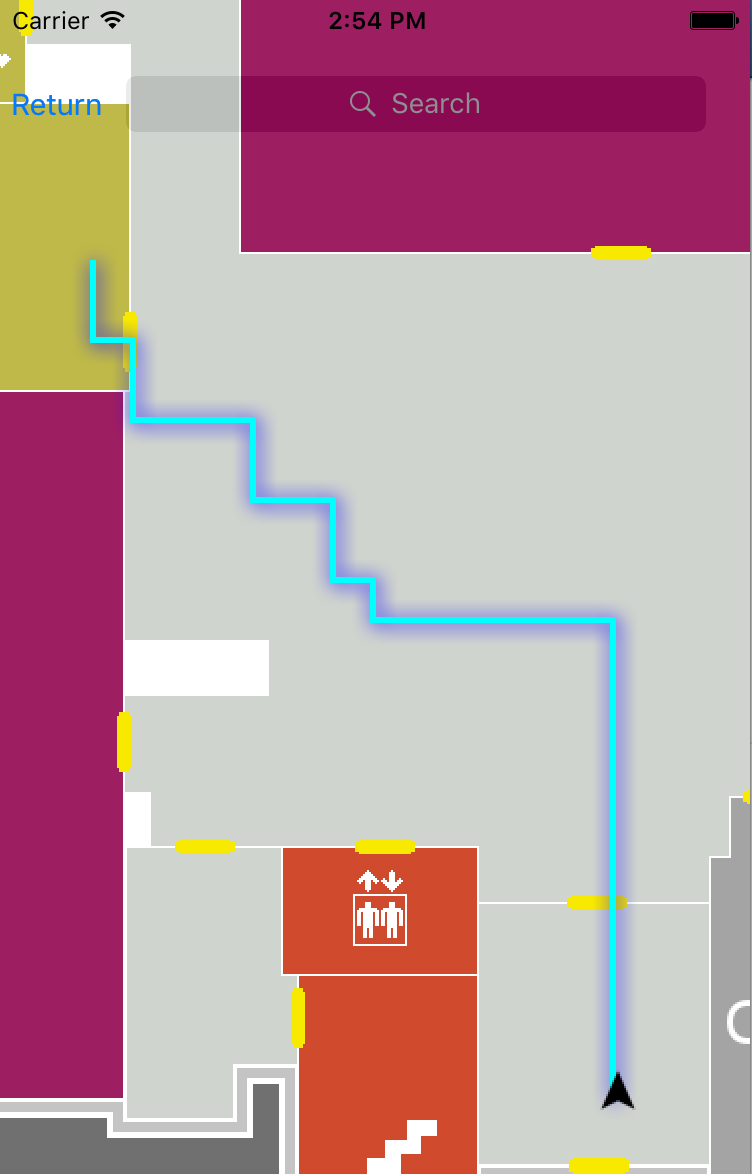
\includegraphics[width=0.5\textwidth]{images/jaggedPath.png}
\caption{Path displayed without path smoothing.}
\label{fig:jaggedPath}
\end{figure}


This made use of the previously mentioned wallCheck() method, which would take a line between two points and check whether it intersects with a wall within the floor plan image. In order to smooth the path, the algorithm first sets the initial point as the start point. Subsequent points are then iterated over and marked as end points. If a line between the set start and end points is shown to pass through a wall at any point, this end point is made the new start point, and the line between the previous start and end points is added to the new smoothed path. Repeating this process until all nodes on the path have been iterated over creates a smoothed path that maximises the spaces between bends in the path. The effects of this smoothing technique are shown within figure ~\ref{fig:smoothPath}.

\begin{figure}[]
\center
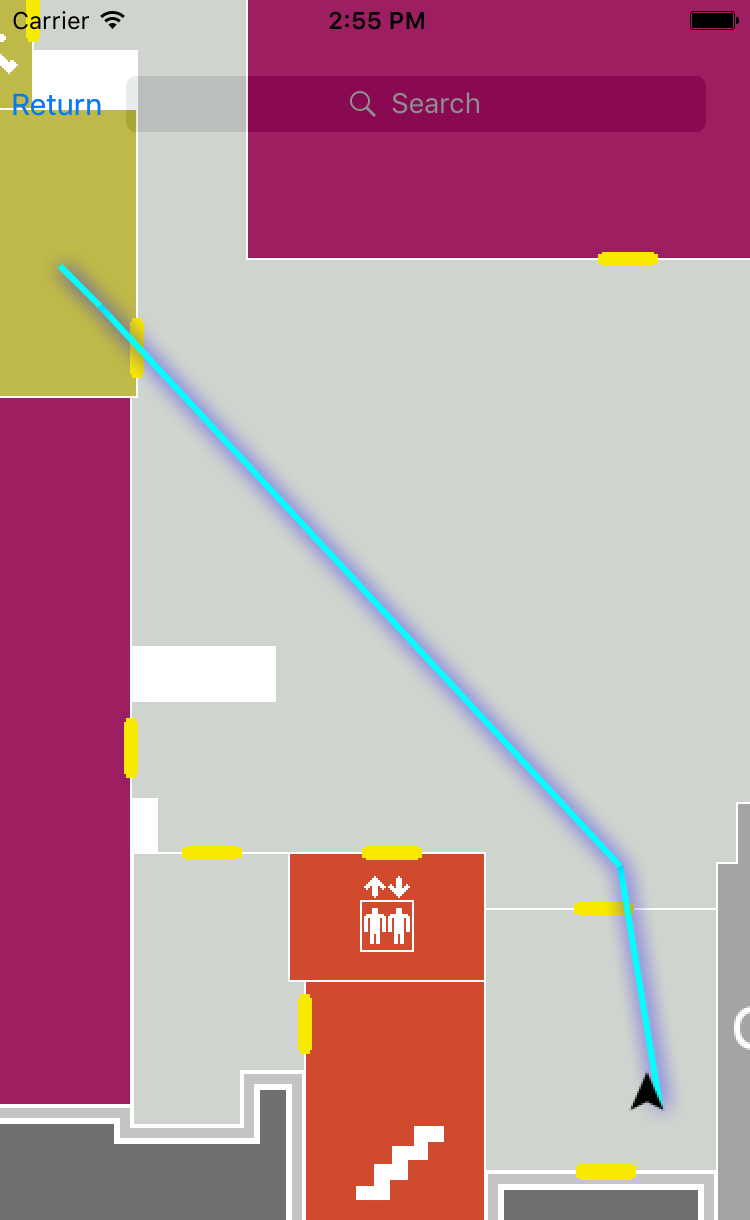
\includegraphics[width=0.5\textwidth]{images/smoothPath.png}
\caption{Path displayed without path smoothing.}
\label{fig:smoothPath}
\end{figure}


\chapter{Testing and Evaluation}

\section{Step Dectection}

Step detection is an integral part of any dead-reckoning system and as such, 
it is prudent to test this particular component in isolation to try and ascertain how much error within the whole system is attributable to the step detection.
As mentioned previously, different methods were implemented to try and find the best step detection system, resulting in three step detection algorithm implmentations that needed testing:
\begin{enumerate}
	\item First Order Low Pass Filter
	\item 10th Order Butterworth Filter
	\item 5th Order Butterworth Filter
\end{enumerate}

Originally, the Basic Peak-Valley detection was also considered for testing as it forms the basis of how steps are detected in all future methods, making it a useful baseline comparison for all results. However, if it is completely unfiltered, then it will simply accept most actions as a step, whilst if it is flitered, then often no action will trigger a step. As such, it is not suited for analysis as a standalone entity, forcing us to forgo these plans.

All tests are done on a device of each operating system (Android/iOS) with six different users. This should allow for these tests to prove that the application works independently of user and device.

\subsection{Error Rate}

The error rate for the Step Detection algorithms is defined as follows:

\begin{equation}
Error\ Rate = 1 - \frac{Counted\ Value}{True\ Value}
\end{equation}

Over a given walk, the number of steps counted by the algorithm is divided by the true value of steps taken to determine the proportion of steps detected. Subtracting this value from 1 gives an overall error rate, with values close to 0 indicating favourable error rates.

%So over a known number of steps, True Value, each algorithm is used and its counted number of steps is used to get it's accuracy. From this is then subtracted from 1 to get the error rate. The purpose is to see over a set distance how much error is present overall regardless of timing or other factors such as speed, location etc... This should help to see how much where in the future the system can be improved.


\begin{table}[ht]
	\begin{tabular}{| c || c | c | c | c | c | c | c | c | c | c | c | c |}
		\hline
		True & \multicolumn{4}{c}{Low Pass} & \multicolumn{4}{|c|}{5th Butterworth} & \multicolumn{4}{c|}{10th Butterworth} \\
		\hline
		 - & Andr. & Err. & iOS & Err. & Andr. & Err. & iOS & Err. & Andr. & Err. & iOS & Err.\\
		\hline
		10 & 9.3 & 0.07 & 9.33 & 0.07 & 10 & 0.0 & 10 & 0.0 & 10 & 0.0 & 10 & 0.0 \\ 		
		25 & 22.8 & 0.09 & 22.5 & 0.1 & 24.5 & 0.02 & 24 & 0.04 & 26 & -0.04 & 25.7 & -0.03 \\ 	
		50 & 46.5 & 0.07 & 47.33 & 0.05 & 48.3 & 0.03 & 47.8 & 0.04 & 51.3 & -0.03 & 47 & 0.06\\ 
		\hline	
	\end{tabular}
	\caption{The average data recorded from all users.}
\end{table}

The above table shows the number of steps the each step detector counter against the true value. Three different true values where selected to see whether distance would have an impact on error build up. The highest true value, 50, was selected because this is roughly at most the number of steps a user will take to navigate within the environment. 

From the table above it can be see that the error remains fairly consistent across the different steps taken. This is somewhat expected, given the accelerometer is not subject to the drift that the gyroscope suffers from. For 10 steps, all algorithms show almost perfect results. As steps increase, it can be clearly seen that both implementations of the butterworth filter are superior to the low pass filter, with the low pass filter showing the largest error rates within both the 25 and 50 steps tests.

Selecting between the 5th and 10th order butterworth filters is more difficult when accounting for error rates alone, since both show similar results, although the 5th order filter is slightly superior. What works against the 10th order filter is the larger 'lag' registered with it  , with the time between taking a step and the step being recorded being greater for the 10th order filter. This is shown in figure ~\ref{fig:pirate}. Given all this, as has been mentioned previously, the 5th order Butterworth filter was selected as the step detection algorithm of choice, and it is the algorithm that was used for all other tests of the application.

\begin{center}
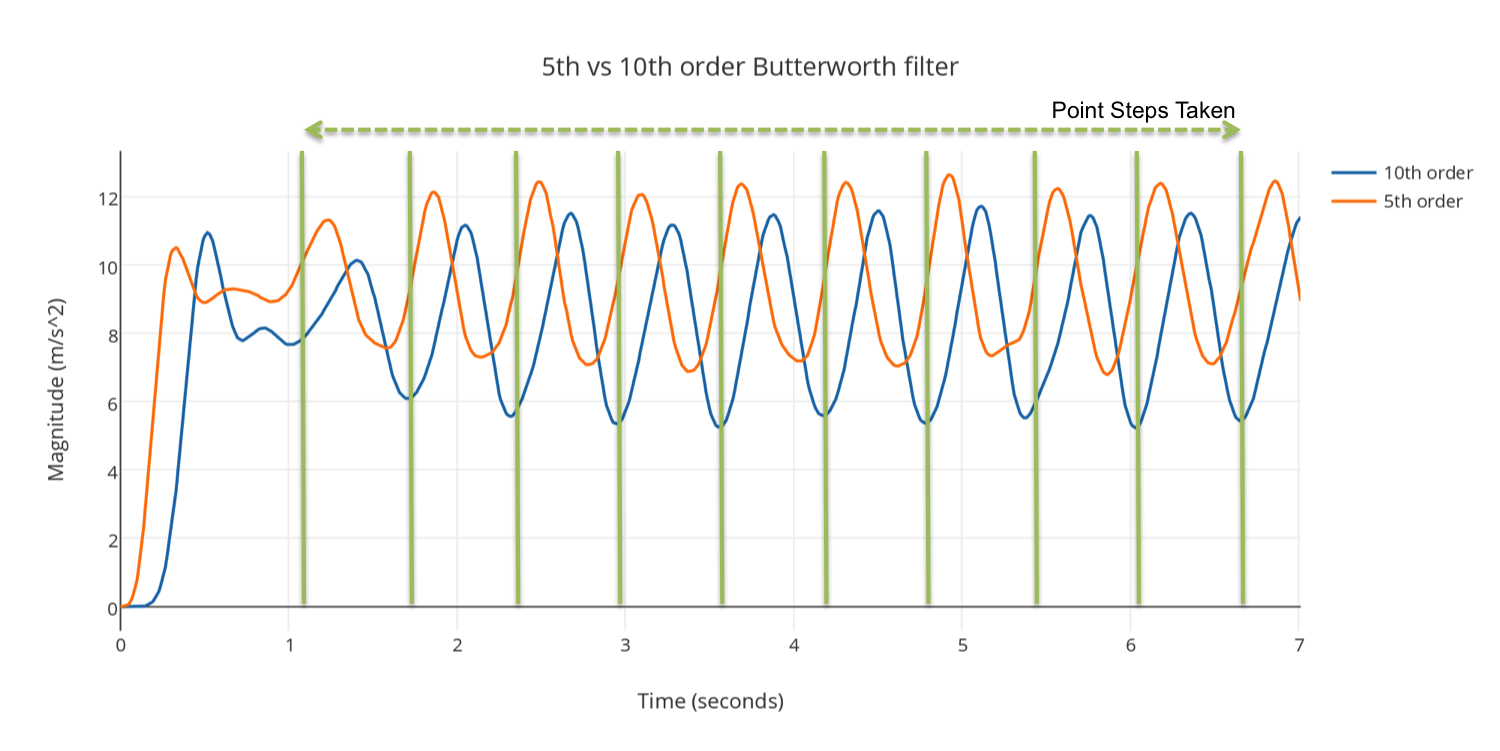
\includegraphics[scale=0.63]{images/pirateResults.png}
\captionof{figure}{Showing steps taken vs when acceleration peak occurs within 5th and 10th order Butterworth filters.}
\label{fig:pirate}
\end{center}

In this particular case, we considered that the underestimation and overestimation of steps are both equally detrimental, since both would result in the addition of an equal amount of error to the system.

%Though overcounting and getting a negative error rate could be considered worse than undercounting. This is because if you overcount it means that for a single step you will have counted an additional step, and in a dead-reckoning system the user will now have moved double the distance in a given direction by your estimate. This could have a larger effect on the error in the system.

\section{Pathfinding algorithm evaluation}

\subsection{Algorithm comparison}
In order to compare the algorithms we selected, we devised a series of tests that allowed us to verify the validity of a given algorithm, as well as its performance and requirements for computation. Our test mesh was the ground floor of DCS, with 19 thousand nodes and 32 thousand edges. We selected this as our testing dataset in order to simulate the application of the algorithm we desired in a closed environment. The tests performed consisted of three stages: 

\begin{itemize}
	\item The first stage dealt with a simple validity check, where we forced the algorithm to find a path between two points. While this test was simplistic, it allowed us to see if all of the algorithms were behaving as expected. 
	\item The second test was based on placing the start and finish next to each other and dividing them by a wall. It was introduced after a behaviour in QuickGraph was observed, where some path finding observers introduced new edges with combined cost if a limit was reached. Therefore, this was a sanity test in order to ensure that this behaviour did not occur with the other observers.
	\item Lastly a full cross-floor test was created. This navigated from the bottom left corner of our mesh to the top right corner. This was the only test that produced noticeable differences in our benchmarks and therefore it had a heavy impact on our decision making.
\end{itemize}

It is important to note that each of the tests were ran 1000 times on the Nexus7 lent to us by DCS. This ensured that the test results were less prone to random fluctuations, as well as allowing us to use the device performance as a direct measure for comparison with further tests. During the series of tests we were also observing other measures such as peak memory allocated during the run of the application, as well as turnaround times.

\begin{figure}[]
\center
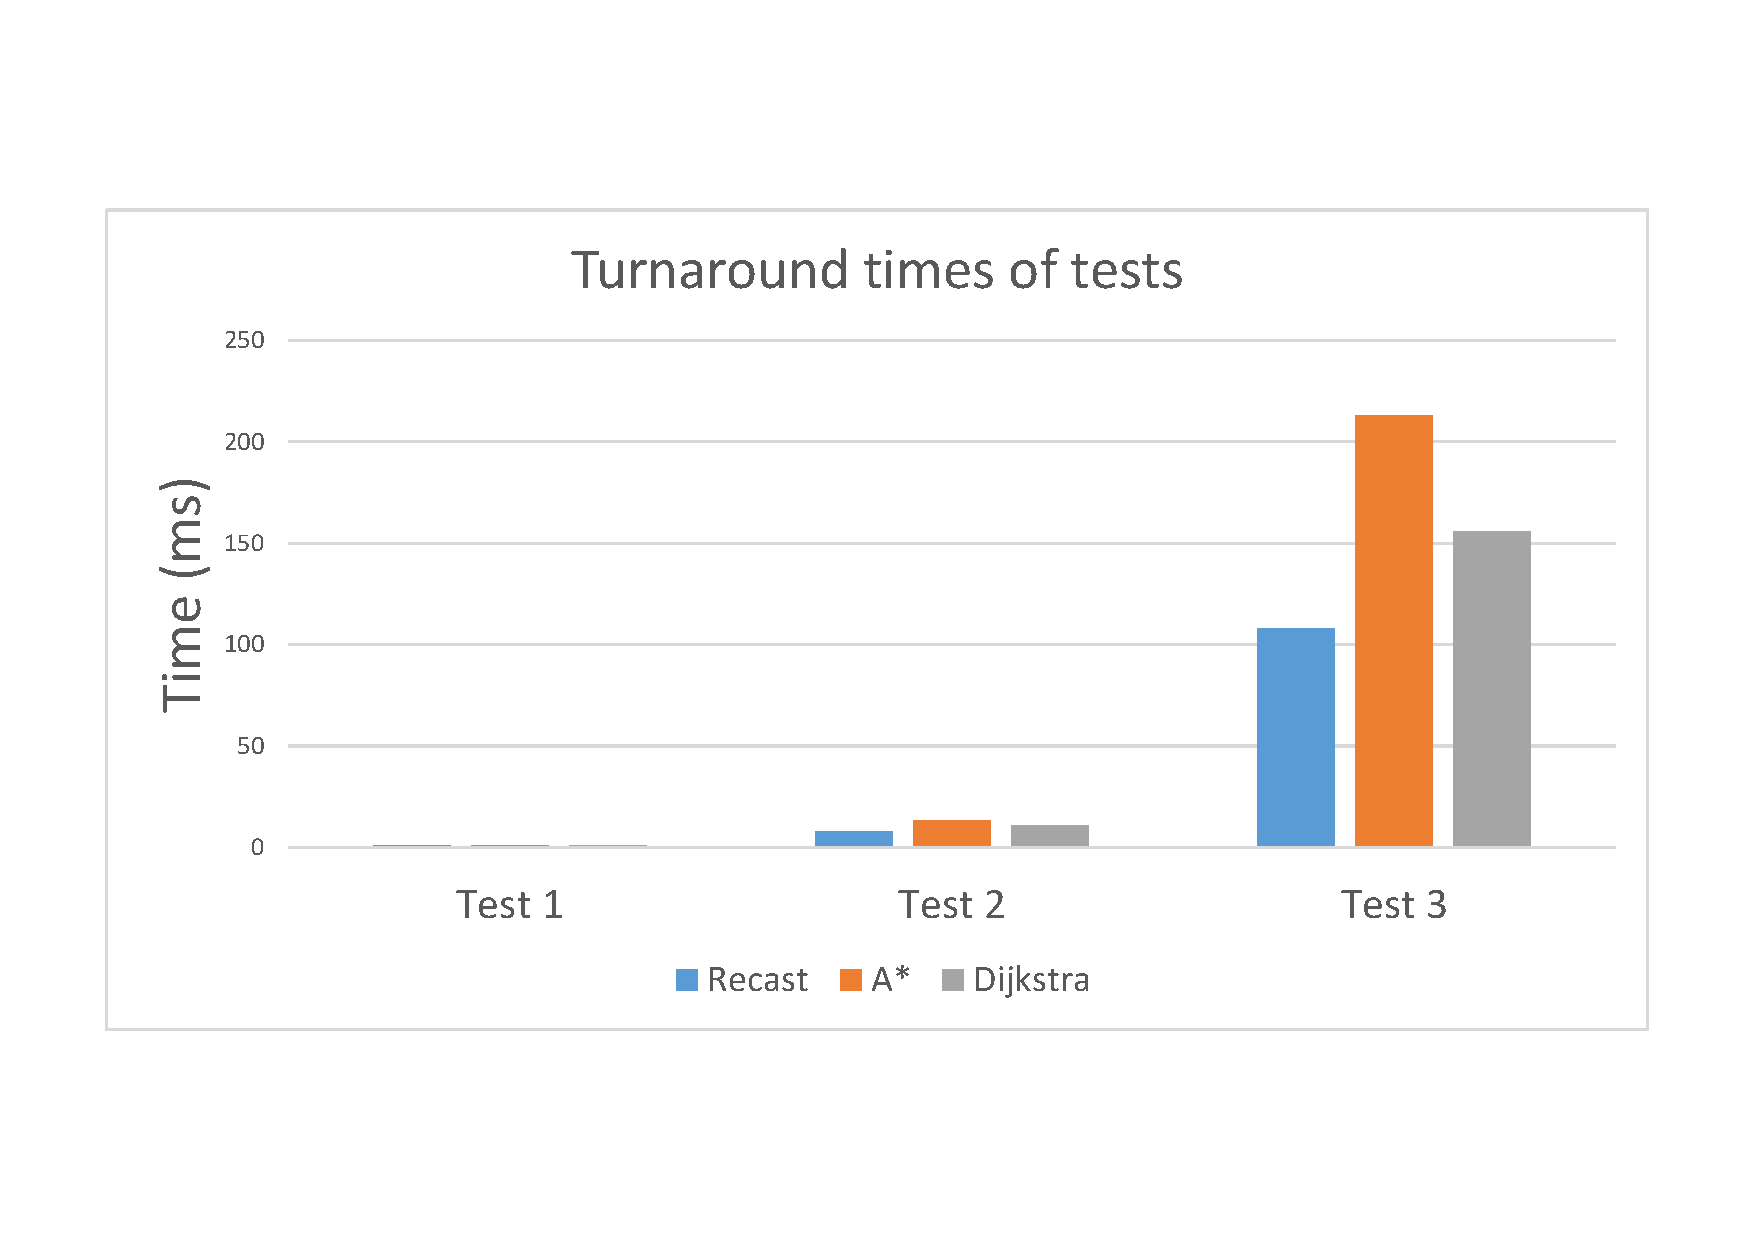
\includegraphics[trim=0 0 0 0, clip,width=0.8\textwidth,height=\textheight,keepaspectratio]{images/algoTurnaroundTimes.pdf}
\caption{Average times required by algorithms to return from computing tests.}
\label{fig:algoTurnaround}
\end{figure}

\begin{figure}[]
\center
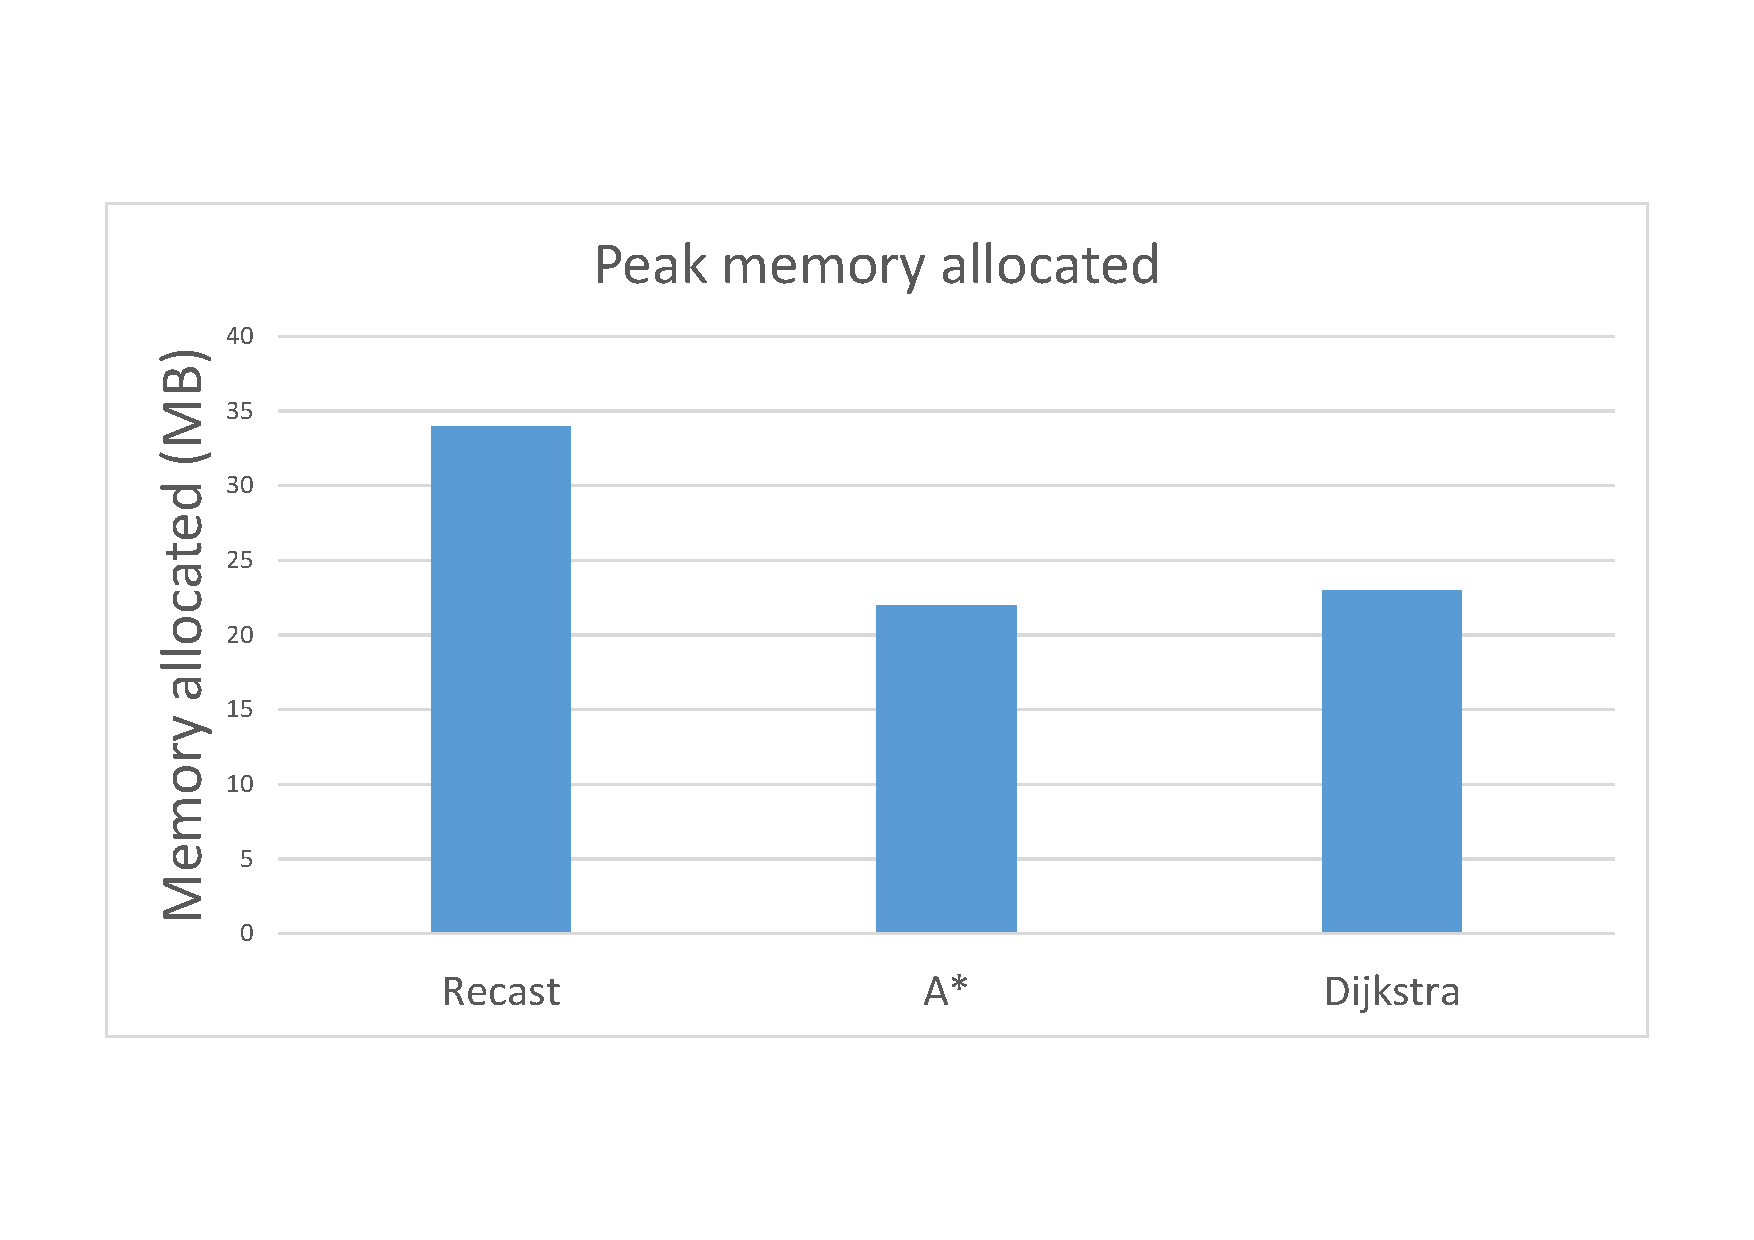
\includegraphics[trim=0 0 0 0, clip,width=0.8\textwidth,height=\textheight,keepaspectratio]{images/algoMemoryAlloc.pdf}
\caption{The maximum amount of memory specific algorithm (and libraries it loaded) required during its execution.}
\label{fig:algoMemAlloc}
\end{figure}

The results of our tests in figure[\ref{fig:algoTurnaround}] show that Recast is able to outperform both Dijkstra and A*, however it also comes with a significantly larger payload thanks to packing the whole Urho library with itself, as well as the memory required for pre-processing the graph. This therefore results in a 50\% larger memory requirement than the second highest competitor, Dijkstra. This can be seen in figure[\ref{fig:algoMemAlloc}]. While this might seem like a reasonable cost to pay for the performance benefit, for a mobile device in which memory is a much more limited resource it is too large. Therefore, we have decided to not go with Recast. Between A* and Dijkstra, the difference in memory allocated is negligible, and Dijkstra outperforms A* thanks to caching provided by the library. In our tests, A* also underperformed due to the large amount of walls in the floor plans, where it tried to utilize its predictive heuristic function to get closer to the target. From our testing we therefore decided to make use of the QuickGraph library, together with the provided Dijkstra observer. 

\subsection{Proximity to Destination}

Having established that the 5th order Butterworth filter was the most appropriate algorithm for use, we proceeded to test the full application. It was tested along a series of routes that fell into two different categories:

\begin{enumerate}
	\item Room-to-Room, so from the entrance of one room to another  %, on the same floor
	\item Point-to-Point, from a specific starting location to a specific destination  %, on the same floor
%	\item Room to Room, across multiple floors
%	\item Point to Point across multiple floors
\end{enumerate}

We again had six different users walking along these routes. Upon the application stating that the destination had been reached, the distance between the users location and the actual location of the destination was measured in metres.

The purpose of this final test was to examine how well the application worked as a whole. The closer the proximity between the user's final location and the desired location, the more accurate the system can be deemed to be.

\begin{table}[ht]
	\begin{tabular}{| c || c | c | c | c |}
		\hline
		Route Number & Starting Location & Ending Location & Route Type & Proximity (m) \\
		\hline
		1 & CS0.06 & CS0.02 & RTR & 1.1 \\
		2 & CS0.03 (Top Right) & CS0.02 (Middle) & PTP & 3.4 (7.0) \\
		3 & CS0.07 & CS0.01 & RTR & 1.4 \\
		4 & CS0.06 (Bottom Left) & CS0.01 (Top Right) & PTP & 2.5\\ 
		5 & Entrance & Stairs & RTR & 1.7 \\
		5 & Stairs & CS1.16 & RTR & 2.6 (5.4) \\
		\hline
	\end{tabular}
	\label{tab:routes}
	\caption{The average proximity to destination, PTP means Point-to-Point, RTR means Room-to-Room}
\end{table}
%Results

Table ~\ref{tab:routes} shows the average distance to the destination for all users across the described routes (with each route being walked three times by each user). Some of the routes are shown in Figure [X]. The description in brackets for the PTP routes is the rough area of the room that the starting or ending location was placed. 5 routes in total were used, with the duplication of the route number 5 indicating a multi-floor route.

As can be seen, the overall error of the navigation for these routes ranged between 1m and 3.5m. In most cases, despite this error, navigation took the user within visual range of the desired destination, meaning that in a real world situation navigation would in most cases have been successful.

Two of the routes within the table have additional proximity values given within brackets. These are the rough distance away from the destination where the application stopped being able to track the user.  These instances occured when the system incorrectly believed the user to be facing a wall, cause all subsequent steps to trigger the wall collision mechanism and effectively cause the user to stop being tracked. This resulted from incorrect compass headings being recorded. We found that in certain locations around the computer science department building, specific areas of magnetic interference caused compass readings to fluctuate and become incorrect. These areas are shown in Figure ~\ref{fig:figureX}.

\begin{center}
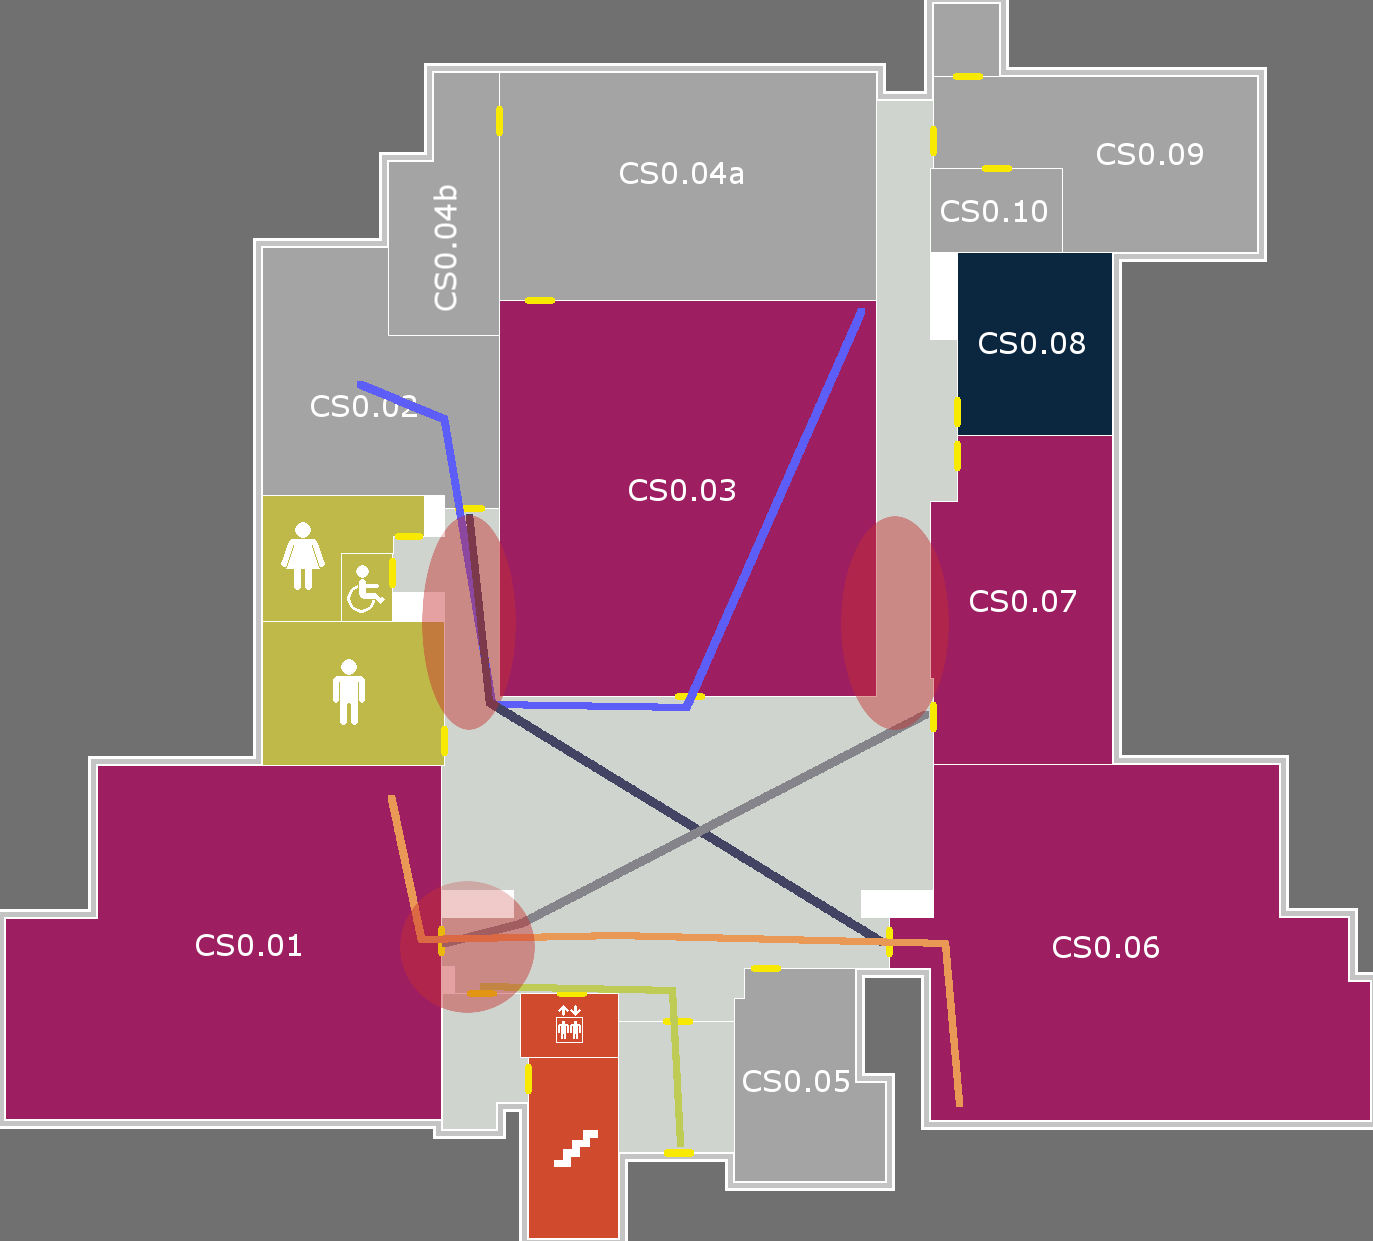
\includegraphics[scale=0.3]{images/figureX.png}
\captionof{figure}{Shows routes taken during testing. Red circles indicate encountered areas of magnetic interference with the compass.}
\label{fig:figureX}
\end{center}

These areas mean that dependening on the route taken by the user, it is possible for the error to cause significant problems. In cases where turns are made around narrow corners or small doorways are present in regions of magnetic interference, such as in route 2, these heading fluctuations cause the wall collision to be triggered and for tracking to fail. In route 1, where no such conditions exist, this problem does not occur. This phenomenon is shown within Figure ~\ref{fig:figureY}.

\begin{center}
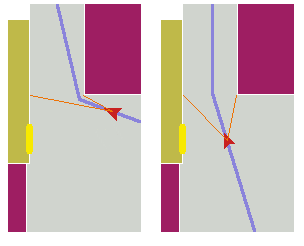
\includegraphics[scale=0.8]{images/figureY.png}
\captionof{figure}{The left side of the image demonstrates  that a sharper turn has a smaller range of heading error that will allow it to navigate the turn effectively. The image on the right demonstrates how reducing the steepness of the turn increases this range of error permitted for the turn to still take place.}
\label{fig:figureY}
\end{center}

Since our environment has several of these large pockets of interference, the application was tested in the concourse of the University Physics building, a location with less electronic equipment, the map of which is shown in Figure [Z]. The testing in this environment was to simply walk around, from a start point, with the phone facing a particular direction and see how the heading changed and the application tracked our location.

\begin{center}
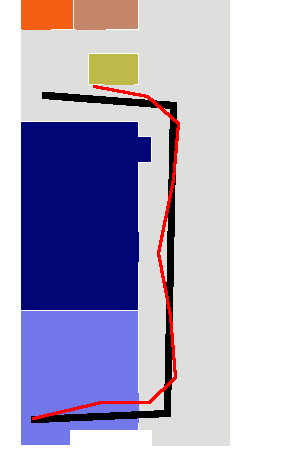
\includegraphics[scale=1]{images/figureZ.png}
\captionof{figure}{Floor plan of science concourse used to perform further tests on the compass.}
\label{fig:figureZ}
\end{center}

Despite having less electronic equipment in the area, we still noticed areas in which the compass value would incorrectly vary by as much as 20 degrees. Therefore, we can assume this interference is an artifact of the architecture and electricy used within the university's buildings. Overall this was an unexpected find. Early testing had failed to indicate such issues with the use of the compass, and from a theoretical perspective, we believed that any magnetic interefere would manifest in a more general offset rather than within small regions giving large spikes in readings.

With consistent compass readings, the system is however shown to be relatively accurate, wtll all completed navigation directing users to within visual contact of their targeted destinations.

\subsection{Other Considered Tests}

Two other tests where considered for use, but ultimately decided against for different reasons. The first was trying to measure if each step detector method was overcounting, registering multiple steps instead when it should only register a single. This is different from what was defined as a false positive earlier where a step is counted when no movement is occuring. This was considered as an alternative to the false positive rate as it looks at the way in which a bad algorithm could have a low error rate but not count correctly. 

However whilst this method could provide some analysis, it was not used for two reasons:

\begin{enumerate}
	\item All the methods being tested do not overcount often, it only really differentiates them from the basic unfiltered version.
	\item The second test that was not used would be better at showing which algorithms are working correctly
\end{enumerate}

The second test that was excluded was aiming to see if step detectors worked effectively over a period of time. The experiment was based off the fact that a person moving at a constant speed will have a repetitive waveform as the input into the algorithms. Therefore the steps being detected should be picked up constantly and equally spaced in time. The purpose of this test is to therefore show that an algorithm is matching the constant pattern and working as intended, it will show up any method that has a low error rate but doesn't work as intended. This was considered a better way to show what the overcounting test would have provided.

Whilst the method had some potential, early data recordings showed that all of the algorithms being tested had roughly the same pattern. They had the same pattern due to the need to have the timing relative to when it itself recorded the first step. Even though some methods recorded steps comparatively longer after they were actually taken, the timing results did not reflect that since the relative difference between when the steps as recorded by the algorithms themselves was similar

\section{Xamarin Forms Evaluation}

Our initial plan was to use the functionality of Xamarin Forms in order to create an application that can be used on both iOS and Android. The appeal of Xamarin Forms is that is provides a hardware independent framework that allows the building of application interfaces using an Extended Application Markup Language (XAML) which has similarities to HTML and other markup languages. This allows for language independent development that is well suited for graphical interface design. Xamarin Forms still requires the use of C\# shared code for most advanced features and in order to link components together. However, coupled with the application independent nature of the shared code, theoretically, one should be able to create applications completely independently of any single platform that relies on the shared C\# code for the back-end and Xamarin Forms for the interface.

\subsection{Issues with Xamarin Forms}

Xamarin Forms is a relatively new development lead by the team at Xamarin and, as such, it is still clearly in its infancy in terms of usability and overall scope. While simple applications that only require basic interface functionality such as lists, simple images and tables are easily created, some advanced concepts are still required to be programmed with architecture specific code, and while Xamarin Forms does account and allow for this, it is somewhat limited when compared to using full native code. Certain simple actions, such as dragging an image around the screen and overlaying images on top of one another, were either very difficult or impossible to implement within the current version of Xamarin Forms.

\subsection{Thoughts on Xamarin Forms}
While Xamarin Forms is an impressive and potentially very useful concept, it is still in its early years and has much scope for improvement before it can be seriously considered as a viable alternative to native code, at least for advanced applications. This is through no fault of the developers however as the scope and difficulty of implementing something like Xamarin Forms is truly commendable and will take many, many man hours and much effort in attempting such an advanced framework. It currently shows great potential and there are many examples of how it can be correctly used in order to create a variety of applications and functionality that will work across multiple platforms.

\subsection{Transition to Shared Project}

Given these difficulties, we shifted work over to a Xamarin shared project from the Forms project. This gave us access to native user interface components of both iOS and Android, and made the process of executing our design ideas much more straight forward, without altering any of the shared code (step detection and path finding for example).

\section{Analysis of Android vs iOS}
As the application created over the course of this project was developed for both the Android and iOS platforms, it is prudent to discuss the respective benefits and drawbacks of each system with regards to various factors.

\subsection{Strengths of the Android Platform}
Whilst there were many problems encountered throughout the project with the Android version of the Navigator application, there were also several positives that were associated with developing for the Android platform.
            
The first of these is that the Android operating system is available for a wide range of devices, including both smartphones and tablet based devices. This allows the final application to be tested on a variety of devices, which is particularly useful to us considering that the Android sub-team all possessed differing smartphones and tablets. In the event that the application is actually released to the public, this property allows the application to cover for a huge potential user base. This is further improved by the backwards compatibility between different iterations of the Android operating system. The level of backwards compatibility is determined by the value of the minimum SDK version set in the file \texttt{AndroidManifest.xml}. In this work, the minimum SDK version and target version were both the same, namely the Ice Cream Sandwich Android release, API level 15.
            
The other major benefit of developing for Android is the open source nature of the platform itself. In addition to the operating system, there are many well supported open source libraries/extensions available, such as the popular `Mono for Android' (sometimes referred to as monodroid by developers). This is useful as there are many situations where specific functionality is not provided by the default Android development environment. Due to the popularity of open  source, however, it is highly likely that there is a freely available implementation of the desired functionality available through services such as GitHub, reducing the complexity of the development process. This was almost the case with implementing proper image scrolling for the floor plan screen, as Mono for Android had some options available. Unfortunately, they were not used due to not fulfilling all of our requirements. We did however make use of an open source version of the Recast algorithm.
       
 \subsection{Drawbacks of the Android Platform}
Over the course of the project we also came across several problems whilst implementing the Android version of our application. One of the most frustrating and time consuming issues encountered was the lack of abstraction provided for dealing with and accessing device sensor readings. For example, obtaining a correct and usable azimuth value was an arduous task (as detailed earlier in this document), requiring the use of specialised classes and mathematics. This is in stark contrast to iOS, which simply allows these values to be accessed through the location manager system, an approach that is far cleaner and more intuitive than the Android alternative. Another issue with sensor access on Android is that the API gives the developer the ability to subscribe to the sensors without the use of a view. This causes problems when a given view is paused as you must re-subscribe to the sensors in use, which can be inconvenient at times. It also has the additional effect of requiring the developer to duplicate code in situations where data from two different views needs to be processed in the exact same manner.
            
Whilst mentioned as a positive earlier on in this section, there are also downsides to the ability of Android to be developed and deployed for a large variety of devices. The primary drawback here is that this means the Android operating system cannot be optimised for specific hardware (as the hardware in question cannot be known ahead  of time), meaning that there are some potential performance problems. However, iOS does not suffer from this issue due to it only being deployed on Apple devices such as the iPhone. Therefore, in terms of overall performance, it is likely that iOS has a slight advantage over the Android platform.
            
Another large problem with the Android system was briefly touched on earlier in this section when discussing open source: there are many features that would be considered fundamental to smartphone usage that are simply not natively implemented for Android. The most problematic of these was the lack of default functionality to properly scroll and zoom large bitmap images (This required the development of a custom tool, discussed earlier). In contrast to this, the iOS image view available through Xamarin Studio handled this by default.    

\section{Summary}

\chapter{Management}

\section{Group Management}
The project group consisted of six members, these were Pedram Amirkhalili, Joseph Benrimoj, Dominic Brown, Varun Golani, Robert Hubinsky and Daniel Seabright. At the onset of the project, Joseph Benrimoj was designated as project manager by way of vote amongst the group.

This initial vote set a trend that continued throughout the project, with democratic votes playing a major part in how work was carried out. Considering the fact that all group members shared an equal stake in the ultimate evaluation and grading of the project, it was felt that all group members had to be happy with both the direction and progress of the project. In addition, it was oftentimes only through unanimous approval that decisions were made. This had the added benefit of having conflicting viewpoints resulting in prolonged discussions about project technicalities and possible design choices. Ultimately, this was a positive, unintended by product of this meeting format, forcing us to go through chains of thought that we may not have otherwise. As with all traditional project teams, any outstanding disputes would be resolved by the project manager.

Considering the small team size and relative inexperience of most group members with development kit (Xamarin), target platforms (iPhone and Android) and the C\# programming language, it was decided that an iterative development model would be best.

Iterative development involves initial implementations of smaller subsets of software requirements, iteratively enhancing ``the evolving versions until the complete system is developed and ready to be deployed'' ~\cite{itDev}. At each subsequent iteration after the initial software subset implementation, design modifications are made and new functionality added and refined. This is the recommended development model when a new technology is being simultaneously learnt and used by a development team, and carries with it several advantages.\\

Principal amongst these is that a working model of the system is available form early on in development. This is vital when wishing to determine whether any functional or design flaws exist, allowing these to be caught early and rectified at the earliest opportunity. Indeed, as has been explained, this was the case within the project, with the iterative development process helping in identifying the problem earlier than would otherwise have been possible.

Testing also becomes easier. Each iteration of development necessarily requires substantial testing to occur, with most of the those tests being on work carried out from the last iteration. This means tests occur periodically and in smaller grouped quantities, making them more manageable, especially for a small team.

Furthermore, as has been alluded to, the evolutionary nature of the project and software matches the gradual evolution of the team's skills in the new technology being used, complimenting the learning process and permitting work to take place concurrently.

Despite these points this model makes project management slightly more complex, with greater emphasis on time management and team communication. This fell principally on the project manager, whose job it was to arrange team meetings and facilitate communication between team members.

Communications occured primarily via the use of social media. Announcements about meetings would be placed within a group chat that all members had access to. Here, the project manager would present possible times for meetings with group members all announcing their availability at those times. Meetings would than be arranged once all group members could attend. These face to face meetings occured once a week and were where the majority of the major project decision would take place. Here issues would be dicussed (such as the work conducted over the previous week) and major decision taken with a vote. On the basis of these decisions, work would then be assigned amongst group members.

When group members were not all on site in order to carry out the face to face meetings, these would be conducted over Skype. Skype calls were also used for work that was done jointly by group members on the same task.
 
 Group roles evolved as work progressed, with these ultimately settling into the following:
 
 iOS development - Joseph and Daniel.\\
 Android Development - Dominic and Robert. \\
 Floorplan Curation - Pedram. \\
 Floorplan graph extraction - Robert. \\
 Step Detection - Varun and Pedram.\\

Work that needed doing would usually be distributed in accordance with these roles. However considering the interconnectedness of components, most group members have had a hand in all aspects of the project.

Communication with the project supervisor occured primarily via email, with face to face meetings occuring on average once every two weeks.

Version control was done using Github, with all group members working on the same repository and in most cases working on the same project branch at all times.

\section{Risk Analysis}
    As with all large projects, a risk analysis was conducted. This is shown in table \ref{tab:risk}.
    \begin{table}[h]
        \centering
        \caption{Risk analysis table}
        \label{tab:risk}
        \begin{tabularx}{\textwidth}{|c|c|c| X |}
            \hline 
            \textbf{Risk} & \textbf{Likelihood} & \textbf{Severity} & \textbf{Mitigations} \\ 
            \hline \hline
            Code Loss & Low & High &
            \begin{itemize}[leftmargin=*]
                \item Store code in online GitHub repository
                \item Maintain multiple hard copies on external media
                \item Regularly commit working software changes
            \end{itemize}
            \\ 
            \hline 
            Delays in progress & Moderate & Moderate &
            \begin{itemize}[leftmargin=*]
                \item Timetable Gantt chart carefully
                \item Dedicate an appropriate amount of time to the project per week
                \item Create timetable with contingency in mind in order to reduce the impact of delays
            \end{itemize}        
            \\ 
            \hline 
            Team member illness & Very Low & Moderate &
            \begin{itemize}[leftmargin=*]
                \item Where necessary, work can be redistributed to other members of the team who are familiar with the specific task
                \item Timetabling contingency can also reduce the impact of this risk
            \end{itemize}        
            \\ 
            \hline 
            Inability to obtain licenses & Moderate & High &
            \begin{itemize}[leftmargin=*]
                \item Use open source software where possible
            \end{itemize}        
            \\ 
            \hline 
            Device breakage & Low & Moderate &
            \begin{itemize}[leftmargin=*]
                \item Some testing can be carried out using emulation software
                \item The team has access to multiple Android and iOS devices
            \end{itemize}        
            \\ 
            \hline 
        \end{tabularx}
    \end{table}

\section{Contingency Planning}

As with any project, contingency planning is an important component of good project management. From the onset of our decision to pursue a Xamarin Forms application as a solution for our project, we knew that we required an effective contingency plan to mitigate against this option not working to our satisfaction. Attracted by the prospect of a shared interface across all iPhone and Android devices (as advertised as possible by the Xamarin website), we were nevertheless sceptical about its ability to handle the more complex user interface requirements of the final application.

With this in mind, we were satisfied with the ability to transfer over to a Xamarin shared project from a Xamarin Forms project. A Xamarin shared project would use the same `shared code', that is, code related to components such as step detection and path finding while making use of native components of each platform in order to construct the user interface.

Given the issues that were ultimately encountered with the Xamarin Forms project, this proved to be a shrewd piece of contingency planning, allowing the project to be realligned to a Xamarin shared project within a period of a week or two and for work to continue effectively from that point.

\section{Implementation Organisation}
Before work began on the implementation of the various main components of the final indoor navigation application, time was spent early on setting up the project and finding our feet with regards to Xamarin.
%This section will detail the process of turning our designs into a working application. It will mostly read chronologically, with tasks and components completed earlier into the project also appearing earlier within this section. This will also aid in demonstrating our thought process behind changes to the application design that arose through development, be it through complications or the realisation of superior design choices.

\subsection{Implementation phases}

Actual application development on this project began with the creation of a data logging application. This would be used to gather principally accelerometer data about steps during walking cycles that would form the basis of the development of the step detection algorithm.

Work around this data logging and initial step detection algorithm implementation comprised phase one of our implementation, with phase two encompassing the development of our main, final application.

\subsection{Obtaining Xamarin License}

We initially experienced many problems obtaining a licensed version of Xamarin, even before proper work began on the actual application. All team members were required to register as a developer on the Xamarin website and request a student developer license, a convenient alternative to the costly traditional license offered to non-students. This involved a prolonged series of exchanges with the company via email, which after 2-3 weeks proved to be a futile endeavour, as we were then instructed to procure the license through alternative means via a third party distributor. Ultimately, it took a few weeks before any of the team were able to obtain a development license, during which time we were able to develop, but not deploy an application to device. 

%Considering this stage of the project was mainly about gathering data through smartphones, this was a disappointing early delay for which Xamarin apologised, citing their newly formed integration with Microsoft Dreamspark as having caused the delays in license distribution.\\

\subsection{Setting Up The Project}

We began by setting up a Xamarin Forms project, which would enable the creation of a shared user interface across iOS and Android. Within a Xamarin Forms project, the user interface is created via scripting in Extensible Markup Language (XML), which allows for the quick creation of text based displays. Here we followed our initial designs, and established a display page that saw a compass image sit at the top of the screen, with gyroscope and accelerometer readings appearing below it. Below those readings lay buttons that allowed for the data being read to be saved to a file. Buttons were also placed so that this file could be labelled in accordance with the movement being performed, for example `Slow Walk' or `Turning a Corner Left`.  These would help identify what each file related to when it came to analysing the data. The compass image was made to rotate with changing compass readings in order to mimic a real world compass.

This interface was developed within the shared code section of the Xamarin Forms project. In order for data values to be recorded, the sensors needed to be individually set up within the iOS and Android code sections. Within iOS, the sensors are accessed via the CMMotion API, whilst in Android, the SensorManager class from the Android.Hardware library is used. These values are passed to the shared code where the XML is updated in order to update the screen display.

Data logging was made a threaded process for the benefit of application performance. Recorded data was placed within an text file comprising of seven columns - time and the x, y and z values from both the accelerometer and gyroscope data. In the case of iOS, accelerometer values are given in terms of units of gravity (G) rather than the rate of acceleration ($m/s^2$) given within Android. For the sake of consistency, these were then converted to values of acceleration by multiplying these values by 9.8.

\subsection{Effect of Dropping Android}
FILL THIS

\chapter{Conclusion}

\nocite{*}

\bibliographystyle{plain}
\bibliography{main}


\end{document}